\documentclass[10pt,a4paper]{book}
\usepackage[utf8]{inputenc}
\usepackage{amsmath}
\usepackage{amsfonts}
\usepackage{amssymb}
\usepackage{graphicx}
\usepackage{CJKutf8}
\usepackage{array}
\usepackage[pdftex,unicode]{hyperref}
\hypersetup{
colorlinks=true,
linkcolor=blue,
urlcolor=blue
}

\usepackage[nonumberlist,nopostdot,toc]{glossaries}
\makeglossaries
\setglossarystyle{altlist}

\usepackage{wallpaper}
\usepackage[vmargin=3.6cm,rmargin=3.6cm,lmargin=3.6cm]{geometry}
\usepackage{float}

\usepackage{titlesec}

%\usepackage{hyperref}

\setlength{\parskip}{0.3cm}

\renewcommand*\contentsname{目錄}

\renewcommand{\figurename}{圖}

\titleformat{\chapter}[display]{\huge\bf}{\arabic{chapter}}{0.5cm}{}

\CenterWallPaper{1}{Pics/background}

\newglossaryentry{Amtrak}
{
  name={Amtrak},
  description={美國國家鐵路。距離 UC San Diego 最近的一站在 Solana Beach。}
}

\newglossaryentry{ARCH}
{
  name={Associated Residential Community Housing},
  description={UC San Diego 住宿組及負責宿舍的處室。簡稱 ARCH,本冊中亦使用 housing 或 housing office 稱之。}
}

\newglossaryentry{Biomed Library}
{
  name={Biomedical Library},
  description={學校圖書館分館。慣稱 Biomed。在 School of Medicine。有研究生專屬自習區。}
}

\newglossaryentry{Bank of America}
{
  name={Bank of America},
  description={銀行名。簡稱 BoA。}
}

\newglossaryentry{Chase}
{
  name={JPMorgan \& Chase},
  description={銀行名。簡稱 Chase。}
}

\newglossaryentry{Coast}
{
  name={Coast Apartments},
  description={UC San Diego 研究生宿舍名。簡稱 Coast。位於 Scripps Oceanography Institute 的校分部。}
}

\newglossaryentry{DS-2019}
{
  name={DS-2019},
  description={申請 J-1 交換學生簽證使用之表單名。}
}

\newglossaryentry{DMV}
{
  name={Department of Motor Vehicles},
  description={類似台灣監理站,提供考駕照註冊車子等服務。簡稱 DMV。}
}

\newglossaryentry{F-1}
{
  name={F-1 visa},
  description={留學生簽證。}
}

\newglossaryentry{Geisel}
{
  name={Geisel Library},
  description={UC San Diego 總圖書館,在 University Center,Library Walk 的底端,為 UC San Diego 最著名的地標。}
}

\newglossaryentry{I-20}
{
  name={I-20},
  description={留學生申請簽證(F-1 visa)時的入學證明文件。}
}

\newglossaryentry{I-Center}
{
  name={International Center},
  description={UC San Diego 國際學生事務中心。簡稱 I-Center。位於 Library Walk 上。}
}

\newglossaryentry{I-94}
{
  name={I-94},
  description={出入境登記卡。(現已電子化。)}
}

\newglossaryentry{J-1}
{
  name={J-1 visa},
  description={交換學生簽證。}
}

\newglossaryentry{La Jolla Village Square}
{
  name={La Jolla Village Square},
  description={位於學校附近的購物廣場名。}
}

\newglossaryentry{LAX}
{
  name={Los Angeles International Airport},
  description={洛杉磯國際機場。機場代號 LAX。}
}

\newglossaryentry{OMS}
{
  name={One Miramar Street Apartments},
  description={UC San Diego 研究生宿舍名。與校總區隔著 5 號州際高速公路。簡稱 OMS。與 Mesa Apartments 相鄰。}
}

\newglossaryentry{PID}
{
  name={PID},
  description={學號。}
}

\newglossaryentry{Price Center}
{
  name={Price Center},
  description={UC San Diego 主要商店、餐廳群及校內 Chase 銀行所在處。位於 University Center。簡稱 PC。}
}

\newglossaryentry{Main Gym}
{
  name={Main Gym},
  description={UC San Diego 體育館主館,位於 Muir College。}
}

\newglossaryentry{Mesa}
{
  name={Mesa Apartments},
  description={UC San Diego 研究生宿舍名。與校總區隔著 5 號州際高速公路。簡稱 Mesa。與 One Miramar Street Apartments 相鄰。}
}

\newglossaryentry{Mitsuwa}
{
  name={Mitsuwa},
  description={日本超市名。}
}

\newglossaryentry{MTS}
{
  name={San Diego Metropolitan Transit System},
  description={San Diego 大眾交通運輸系統。簡稱 SDMTS 或 MTS。含公車與輕軌系統。UC San Diego 附近僅有公車路線營運。}
}

\newglossaryentry{NCTD}
{
  name={North County Transport District},
  description={San Diego 北部市郊私營大眾交通運輸系統。簡稱 NCTD。含公車路線與火車。}
}

\newglossaryentry{Ralphs}
{
  name={Ralphs},
  description={美國超市名。}
}

\newglossaryentry{Ranch 99}
{
  name={Ranch 99},
  description={華人超市名。又稱大華超市。}
}

\newglossaryentry{Rita}
{
  name={Rita Atkinson Residences},
  description={UC San Diego 研究生宿舍名。簡稱 Rita。位於校內 School of Medicine 區域。}
}

\newglossaryentry{RIMAC}
{
  name={RIMAC Gym},
  description={UC San Diego 體育館名。位於 North Campus。為校內佔地最大的體育館。}
}

\newglossaryentry{SAN}
{
  name={San Diego International Airport},
  description={聖地牙哥國際機場。機場代號 SAN。}
}

\newglossaryentry{SSN}
{
  name={social security number},
  description={社會安全碼。簡稱 SSN。功能類似國內身份證編號。}
}

\newglossaryentry{SDGE}
{
  name={San Diego Gas \& Electric},
  description={營運 UC San Diego 宿舍區水電的公司。簡稱 SDGE。}
}

\newglossaryentry{SGA}
{
  name={Single Graduate Apartments},
  description={UC San Diego 研究生宿舍名。簡稱 SGA。位於校內 Warren College 區域,鄰接工學院。}
}

\newglossaryentry{TGSA}
{
  name={Taiwanese Graduate Student Association},
  description={台灣研究生學會。簡稱 TGSA。美國其它大學亦有類似組織,本冊中指 UC San Diego 台灣研究生學會。}
}

\newglossaryentry{T-Mobile}
{
  name={T-Mobile},
  description={電信公司名。}
}

\newglossaryentry{Trader Joe's}
{
  name={Trader Joe's},
  description={美國超市名。}
}

\newglossaryentry{TritonLink}
{
  name={TritonLink},
  description={UC San Diego 學生事務的入口網站,選課、繳學費等等都可從這裡線上辦理。}
}

\newglossaryentry{UTA}
{
  name={United Taiwanese Association},
  description={(大學部)台灣學生會。簡稱 UTA。本冊中指 UC San Diego 台灣學生會。}
}

\newglossaryentry{UTC}
{
  name={University Town Center},
  description={位於 UC San Diego 附近的大型購物商場名,也是 MTS 公車總站。簡稱 UTC。}
}

\newglossaryentry{Wells Fargo}
{
  name={Wells Fargo},
  description={銀行名。}
}

\newglossaryentry{Verizon}
{
  name={Verizon},
  description={電信公司名。}
}

\newglossaryentry{VONS}
{
  name={VONS},
  description={美國超市名。}
}

\newglossaryentry{Zion}
{
  name={Zion},
  description={韓國超市名。}
}


\begin{document}
\begin{CJK}{UTF8}{bkai}

\begin{titlepage}
\clearpage
\vspace*{\fill}
\begin{minipage}{\textwidth}

\begin{center}
\textbf{\huge UC San Diego TGSA 2018 新生手冊}
\vspace{1.5cm}\\ 
\includegraphics[width=\textwidth]{Pics/triton}\\ \vspace{1.5cm}
\textbf{\LARGE 美國加州大學聖地牙哥分校台灣研究生學會}\\ \vspace{0.2cm}
\textbf{\large UCSD Taiwanese Graduate Student Association}
\end{center}

\end{minipage}
\vfill
\clearpage
\end{titlepage}

\frontmatter
\chapter*{UCSD TGSA 2018 幹部名單}

\begin{itemize}
\item email:\url{ucsdtgsa.website@gmail.com}
\item 網站:\url{http://ucsdtgsa.blogspot.com/}
\item Facebook 社團:\url{http://www.facebook.com/groups/13591139149/}
\end{itemize}

{
\setlength\extrarowheight{0.3cm}
\small
\begin{center}
\begin{tabular}{l l p{4cm} l}
\hline
職稱 & 姓名 & 系所 & email\\
\hline

\parbox[t]{3.4cm}{會長\\President} & 王維楨 & \parbox[t]{4cm}{Computer Science \\\& Engineering} & \url{weichen1027@gmail.com} \\


\parbox[t]{3.4cm}{副會長\\Vice President} & 黃哲琳 & \parbox[t]{4cm}{Electrical\\\& Computer Engineering} & \url{tiesto1114@gmail.com} \\
 & 陳鼎崴 & \parbox[t]{4cm}{Master of Business \\\ Administration} & \url{Ting-Wei.Chen@rady.ucsd.edu} \\


\parbox[t]{3.4cm}{活動\\Chief Executive Officer} & 邱詩雅 & \parbox[t]{4cm}{Computer Science\\\& Engineering}& \url{silvia.chyou@gmail.com}\\
& 林致宏 & \parbox[t]{4cm}{Computer Science\\\& Engineering} & \url{chl584@eng.ucsd.edu}\\
& 莊善淯 & \parbox[t]{4cm}{Computer Science\\\& Engineering} & \url{s4chuang@eng.ucsd.edu}\\
& 李季庭 & \parbox[t]{4cm}{Mechanical \\\& Aerospace Engineering} & \url{ctlee130@gmail.com}\\
& 陳炫宇 & \parbox[t]{4cm}{Material Science \\\& Engineering} & \url{wakaharu37@gmail.com}\\
& 劉育佳 & \parbox[t]{4cm}{Chemical Engineering} & \url{liu19901124@gmail.com}\\



\parbox[t]{3.4cm}{財管\\Financial Officer} & 林千涵 & \parbox[t]{4cm}{Computer Science\\\& Engineering}& \url{chl590@eng.ucsd.edu}\\


\parbox[t]{3.4cm}{網管\\Website Administrator} & 謝靖恆 & \parbox[t]{4cm}{Electrical\\\& Computer Engineering} & \url{williewiz81@hotmail.com}\\
\\

\hline
\end{tabular}
\end{center}
}
\newpage
\section*{致謝}

2014 新生手冊初版編輯小組:黃翊柔、方程毅、邵駿澤、施惟元、胡凱婷、陳品瑋、沈佩萱、廖維平、曾紀為、蕭怡萱、黃安、徐聖修、蘇仲岐。\\
2015 新生手冊再版編輯小組:湯宗曄、徐翰泰、黃敬心、姜博翰、羅恩晴、李融宗、廖尉棠、郭植中、江宜達、吳昇峰、余靖涵。\\
2016 新生手冊再版編輯小組:王維楨、黃哲琳、陳鼎崴、謝靖恆、邱詩雅、林致宏、莊善淯、李季庭、陳炫宇、劉育佳、林千涵、胡毓青。\\
2017 新生手冊再版編輯小組:姜力元、陳昶君、李仲妮、陳境馥、柯成霖、林冠伯、劉家穎、魏佳儀、傅蕎、鄒智璿、陳敖丘、高芷涵。\\
2018 新生手冊再版編輯小組:黃俊嘉、賴顗安、王高健、胡鈞、陳喬玲、朱宥繐、江貫榮

非常感謝 2014 編輯小組們的努力,在歷經數個月的資料搜集、撰寫、攝影、排版、校稿之後,讓 UC San Diego TGSA 開始有了屬於自己的新生手冊!

也感謝 2015、2016、2017 小組參與編修與再版,使新生手冊更為完備。

此外也謝謝 TGSA 學長姐在手冊編輯過程中給予的支持與建議。希望初來乍到聖地牙哥的台灣同學們,可以在這本生存指南中找到有用的資訊,幫助同學們在 UC San Diego 展開一段新的人生旅程。

\section*{使用說明}

UC San Diego 2018 TGSA 新生手冊是為各位新生們精心打造的全方位生存指南,除了可供閱讀之用,更提供了豐富的網路資源,可以直接點擊文件內之超連結使用。含超連結文字皆顯示為\href{http://ucsdtgsa.blogspot.com}{藍色},請多加利用! 

\tableofcontents
\mainmatter

\chapter{出國前的準備}
\section{入學手續}
在收到 graduate division 的 admission package 後,學校的申請網站(\href{http://grad.ucsd.edu/admissions/admitted/index.html}{Graduate Division})上會告訴你需要哪些文件才算完成入學手續,以下針對比較可能會有疑惑的幾點稍作說明:

\subsection{GradApply}
Accept admission 之後依照各 program 需求不同,可能會顯示要求上傳不同的文件(有些甚至可能會需要郵寄實體文件)。submit SSN 的部分,沒有的話就不用上傳。(基本上國際生普遍不會有 SSN)

\subsection{I-20}
UCSD 會要錄取的同學自行付郵資寄回台灣或者寄到你在美國可以收件的地方,當你完成入學手續時,\href{https://icenter.ucsd.edu/ispo/new/index.html}{學校網頁}會有清楚的步驟,請新生就依照網站上的步驟即可完成入學手續。
I-20 是申請學生簽證時必備的文件之一,有鑑於美國的行政效率真的不好說,為了避免申請簽證的流程被延誤,建議有學校帳號可以申請時先去申請。

\subsection{Statement of Legal Residence}
這份文件的用途聽說主要是判別你要繳的學費是州內還是州外,因此國際生主要填完基本資料,讓他確認你不是加州人就行了。\\
可以參考\href{https://drive.google.com/file/d/1IEqT0NRcfPAuc9X-UyOSKAY0vkTENlCH/view?usp=sharing}{範本內容},紅框內為需要填寫部分。

\section{申請護照與簽證}

護照相關資訊請參考外交部領事事務局,簽證相關資訊請參考 \ref{sec:visa}。

護照快過期或者役男退伍後,都建議先去辦理新護照再申請美簽,避免到時候要帶兩本護照到美國,省了一點麻煩。

申請美簽去 AIT 時能早到就早到,避開得排隊的人潮,一定要注意的是該帶的東西一定要帶齊(照片記得使用3個月內的正方形照片,若是明顯不像3個月內的照片對方會要求現場重拍)。特別須要注意的是學生簽證只允許各位在開學日(依照 I-20 上的日期為準)的 30 天之前入境美國。如果要以觀光簽證入境美國再轉換成學生身分極為複雜(最快的方法是重新入境)要先來旅遊的同學必須注意並查清楚相關規定。

\section{決定住處}

關於校內宿舍、校外租屋概況,以及如何申請,請參考 \ref{sec:housing}。\\
p.s. 若想要住校內宿舍,建議能盡早就盡早開始排。

\section{訂機票}

正常如果在台灣訂來回機票,期限是一年內要訂好回程機票,舉例來說,你今年訂了 8/29 的機票來美國,那你就要保證自己在明年的 8/29 前回去,不然可能就拿不到來回機票的價錢,所以通常如果你短期內不會返台的話,可以考慮只買單程機票,在美國再買回國的來回機票,如果避開美國假日,例如聖誕節假期,通常會比在台灣買來回票便宜。

距離學校最近的機場是聖地牙哥國際機場(San Diego International Airport,SAN)和洛杉磯國際機場(Los Angeles International Airport,LAX),最近華航還開通加州安大略( Onterio)直飛,以下是幾種比較常見的飛法:

\begin{enumerate}
\item 從台灣至他國轉機後直飛 SD:

最常見的路線是台灣至東京後轉機直飛 SD。SD 機場至 UCSD 約 30 分鐘路程,可以申請學長姐接機、自行搭 Uber 或租車都可以到。

此飛法的好處是可以順便去其他國家帶個伴手禮,不嫌行李重的同學甚至可以考慮過夜然後順便去其他國家玩一下(?)。

* 若有在其他國家過夜的同學請自行注意是否會有簽證問題。

\item 從台灣直飛到 洛杉磯(LAX) 或 舊金山(SFO) 國際機場:

這種飛法的航班會比第一種多很多,不過需要注意的是 LAX 和 SFO 都是大機場,若是選擇在這兩個機場轉機後飛 SAN 的同學記得要留多一點轉機時間(至少3小時以上),買機票的時候也要注意行李可不可以直掛,若是不能直掛的要確認後面那段國內線的行李量有沒有不同。

到達LAX後若不想搭飛機的話,也可以考慮搭乘機場 Flyaway 巴士 (\$8) 、私營機場接駁 shuttle 或是地鐵至 LA Union Station ,再轉搭美國國鐵(Amtrak)到 Solana Beach Station 或 Old Town Station (\$30 -- \$40)然後請學長姐接機或轉公車 101(NCTD Breeze)到 UCSD。

\end{enumerate}

買機票方面可以自行聯絡旅行社或航空公司,或是透過網路購票。有些航空公司會有比較便宜的學生機票,可以申請國際學生證後購買(有關如何申請國際學生證,\href{https://www.isic.hk/home/apply/isic}{此網站}上面有詳細的申請辦法)。另外八月和九月之間飛機票價也會有個明顯的的差距。



\section{體檢}

學校網頁上可以下載一張疫苗注射紀錄表,印出來後連同從衛生所申請的個人疫苗紀錄一起帶到大醫院(大台北地區有台大醫院、馬偕醫院和慈濟醫院)的旅遊醫學科(有些醫院會將旅遊醫學科放在家醫科下),請醫生照著紀錄評斷還需要補打哪些疫苗。其中,部分疫苗可能會需要施打一劑以上(每劑間格2週~數月都有可能),或是有些疫苗不能同時施打,而TB檢測一般需一週,因此檢驗的時間安排上請自行注意。

牙醫方面能在台灣先看過就先看,需要拔的智齒能拔就趕快拔,這邊看醫生非常的貴,若用學校保險可到鄰近的診所免費洗牙。

眼鏡方面能多配幾付也盡量在台灣就先配好,雖然這邊配眼鏡有保險給付,但是要驗光或者給醫生開處方證明就相對比較貴也比較麻煩。有習慣使用日拋/週拋/月拋隱形眼鏡的同學也可以在台灣先買好再帶來美國。

\section{寄包裹}

受到航空公司行裡的重量限制因素,大部分學生都會需要從台灣寄包裹,台灣郵局有提供三種選擇:航空、陸空、海運。價錢的話:航空 $>$ 陸空 $>$ 海運,時間則是航空 $<$ 陸空 $<$ 海運,以 10 公斤為例:

\begin{center}
\begin{tabular}{c c c}
\hline
寄送方式 & 價格 & 需要時間\\
\hline
空運 & 約32XX元 & 10--13天\\
陸空 & 約20XX元 & 21天\\
海運 & 約12XX元 & 75--90天\\
\hline
\end{tabular}
\end{center}

其他快遞公司也有提供國際包裹服務(\href{http://www.fedex.com/tw/}{Fedex}、\href{http://www.dhl.com.tw/zt.html}{DHL} 等等),相對價錢也會稍微高一點,如有需要請自行查各快遞公司的官方網站。

\begin{figure}[b]
\centering
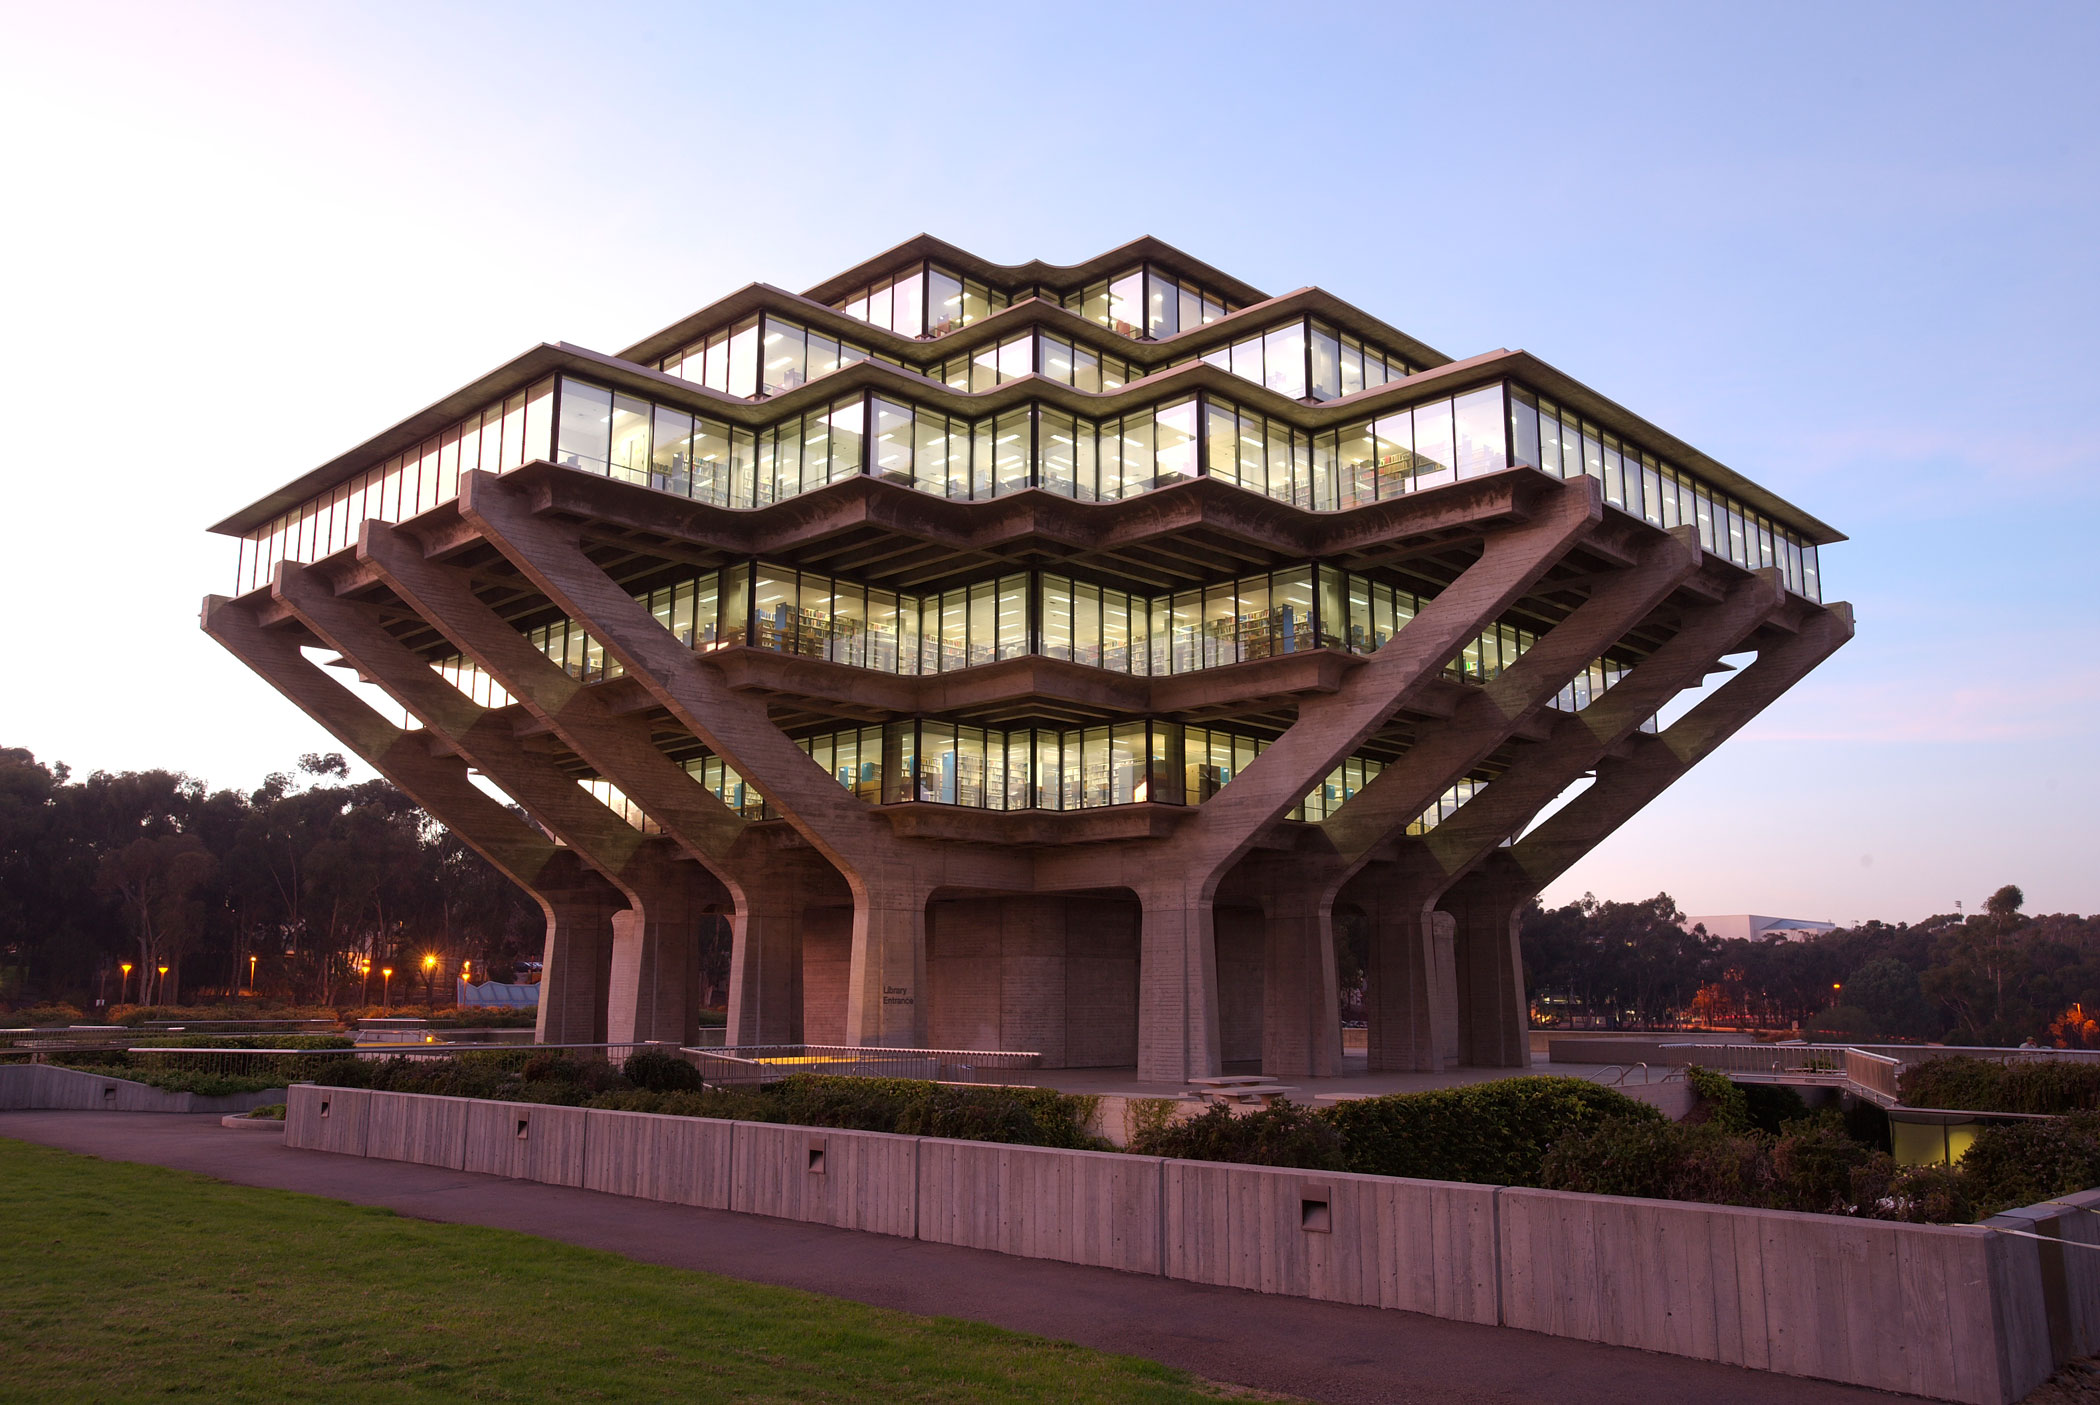
\includegraphics[width=0.9\textwidth]{Pics/geisel-hr}
\caption{UC San Diego 著名的地標---Geisel Library。其命名為紀念晚年在 La Jolla 長住的兒童文學作家 Dr. Seuss。圖片出處:\url{http://publications.ucsd.edu/image-library/campus.php}。}
\end{figure}

\chapter{建議攜帶物品}

\section{證件資料類}

\begin{itemize}
\item 護照。 (如果舊護照上面有以前的美簽需要帶舊護照去面試。)
\item I-20 或 DS-2019。
\item 畢業證書、學歷證明(中英文都需要,到系所報到有可能需要用到,建議出國前先回母校申請幾份英文版的畢業證書影本、學歷證明正本、成績單正本,以備不時之需)。
\item Admission letter。
\item 台灣駕照、國際駕照、英文無肇事證明。
	\begin{itemize}
	\item 在通過駕照筆試後,可以出示台灣駕照與國際駕照直接換發臨時駕照(效力等同正式駕照,但有時間限制)在通過路考前可獨自開車上路,有預計來美就會需要開車的記得要帶台灣駕照(請注意,單就國際駕照本身,只有「翻印本」的性質,本身沒有任何效力)。
	\item 如果沒有台灣駕照與國際駕照的話,在加州只能拿到學習駕照,這邊也有華人駕訓班可報考練習,到時駕訓班會用他們的車送你考試跟練習,開車時需要有持正式駕照或者臨時駕照者在車上陪同。
	\item 英文無肇事駕駛紀錄證明在買車、辦保險、辦駕照時有可能會需要,建議申請一份帶上。
	\end{itemize}
\item 財力證明(有全額獎學金的博班生沒有攜帶財力證明的必要)。
\item 接機人、親友或是台灣同學會聯絡電話、美國宿舍住址。
\item 健康檢查紀錄、疫苗接種記錄。(雖然學校沒有要求,但可在出國前做健康檢查,並攜帶一份英文紀錄以備不時之需。)
\item 國內身份證及其他證件\textbf{可不用帶}。
\item 役男退伍後,已有護照者,可攜帶退伍令、身分證至外交部領事事務局註銷「尚未履行兵役義務出國應經核准」戳記。若出國前沒有註銷,也可以在過海關時直接出示退伍令。
\item 5$\times$5 公分美簽照片(主要)、兩吋、一吋照片(次要)與照片檔案建議可以攜帶\footnote{美國證件多半要求 30 天內的近照、或當場用 webcam 照。美國一般不使用台灣常見的一吋、兩吋大頭照。}。
\end{itemize}

\section{美金與旅行支票}
\begin{itemize}
\item 旅行支票:需要本人雙簽名,可直接當現金使用且比現金安全,若不小心遺失也可憑旅行支票號碼(記得另外記下)申請補發。若是需要攜帶大美金,如學費,建議以旅行支票形式攜帶,來美國之後再直接兌現或存入銀行。
\item 現金:如果攜帶超過一萬美金(各種不計名有價證券,例如支票、不計名旅支、現金)進入美國,入關時需申報,海關可能會要求檢查金額是否與申報的金額相符,若不符,海關有權沒收你的現金。身上最好可以攜帶一些面額較小(\$1--\$20)的鈔票,因為有些商家會不收面額 \$100 的美金鈔票。
基本上在美國消費都可以刷金融卡,所以用到現金的機會很少,可以考慮以旅行支票為主,到美國後開戶即可使用金融卡消費。
\item 匯款:可以到美國開戶之後,再直接從台灣用匯款的方式把學費、生活費等大額美金匯入美國戶頭。建議開一個儲蓄戶頭跟一個現金戶頭,鄰近的銀行有Bank of America, City Bank,校園內有 Chase Bank 都是常見的大銀行,分行跟ATM都很多很方便。
到美國開戶之後請提供以下資訊給你在台灣的家人或朋友,以方便他們匯錢給你:受款人姓名、銀行全名、開戶銀行地址、routing number、account number、SWIFT code。
\end{itemize}

\section{教科書}
美國教科書價格十分昂貴,大概是台灣的二到三倍以上,若是可以接受電子版教科書的同學,其實可以先在網路上找找看,多數經典的教科書網路上有機會找到免費版本,而電子書版本普遍也比紙本來得便宜。若真希望能閱讀紙本的同學,除了可以帶一些已經有的教科書之外,可以在出國前先調查可能會用到的課本從台灣帶來。但要注意在台灣買可能會有國際版與美國版的差別,雖然內容大同小異,但可能會有章節或是習題的變動,可自己斟酌。

另外,也可等到開學後確定要修的課程,再在台灣的網路書店、拍賣網站購買,或請親朋好友代買後寄到美國。Fedex等快遞或是郵局的國際快捷可以在三天到十天左右拿到書,雖然從台灣郵寄需要運費,但還是會比直接在美國買省下不少書費。或是向已經修過課的學長姊買二手或是商借。

若真的需要在美國購買,可在學校的 Bookstore 購買或上 \href{http://www.amazon.com/}{Amazon}、 \href{http://www.abebooks.com/}{Abebooks}、\href{http://www.dealoz.com/}{DealOz} 網站搜尋。Bookstore 會有當學期各系所開課教授指定的課本,除了新書有時會有二手書或是租書的選擇,價格會比新書便宜一些但仍是偏高。而 Amazon 的新書價格有時會比直接在 Bookstore 購買便宜一些。

\section{文具}
\begin{itemize}
\item 文書類:原子筆、自動筆、筆芯、橡皮擦、修正液/帶。
\begin{itemize}
\item 美國習慣用較粗或是油性的原子筆,用習慣 Pilot、Uni-ball 等日系偏細或水性原子筆的話可考慮多帶一些。美國自動鉛筆大多是 0.7,若從台灣帶自動鉛筆來,最好順便自行準備筆芯。
\end{itemize}
\item 筆記類:筆記本、筆記紙、便利貼、L 夾。
\begin{itemize}
\item 美國筆記本價格較台灣貴,選擇也較少,若有特別偏好的筆記本的話可斟酌行李重量攜帶,或是真的用不習慣再從台灣郵寄。
\item 美國主要使用三孔夾跟三孔紙,不像台灣慣用 26 孔的筆記本跟內頁紙。習慣用 26 孔的話可能需要自行攜帶,不然就是來美國再買即可。
\end{itemize}
\item 工具類:一般或工程計算機、剪刀、美工刀、口紅膠/膠水、膠帶、雙面膠、迴紋針、燕尾夾、釘書機/針等等。
\begin{itemize}
\item 計算機可從台灣帶來,其他工具類則沒有特別需要攜帶,有多餘行李空間再帶即可。
\end{itemize}
\end{itemize}
上述所有文具在美國都可以買到(學校裡面的書店其實有各式各樣的文具用品),但價格普遍偏高,品質可能沒有台灣或日本的好\footnote{若要在 UC San Diego 附近購買較便宜的台灣、日本文具,最近須開車或搭乘公車至 Mira Mesa 之 Daiso 大創百貨購買。}。可以斟酌行李空間跟自己的使用習慣從台灣帶來,來美國後就不需要特地去買。


\section{電子相關產品}
\begin{itemize}
\item 線材。
\begin{itemize}
\item 連接線:美國有些印表機、螢幕不附連接線,可帶著備用。
\item 電源延長線(三孔佳)。
\item 網路線:雖然幾乎是用無線網路,可帶著備用,線長買長一點較方便。
\end{itemize}
\item 筆記型電腦:已經有筆記型電腦就可直接帶來美國,非美國品牌的電腦(如 Acer、ASUS、Toshiba 等)可注意是否有全球保固的服務,若是要在美國維修會較麻煩且金額較高,甚至會需要寄回台灣維修。若是想換新電腦,可到美國再買,價格會比台灣便宜一些,但通常不像台灣會附贈滑鼠、背帶、鍵盤膜等等。鍵盤則只有英文字母,沒有注音符號。美國電壓跟插頭跟台灣相同所以很方便!
在美國買電腦平均下來比台灣便宜一萬元台幣左右,考慮買新電腦的人可以來美國再買,PC 裡的 Bookstore 也有許多選擇,且有學生優惠,通常比外面便宜。
\item 相機:已有的可以直接帶,若想買新的可考慮來美國再買,某些品牌在特價時價格較便宜。
\item 其他周邊:隨身碟、隨身硬碟、行動電源、光碟機等等,則依個人需求攜帶;而印表機、螢幕等大型產品來美後有需要再買即可。
\end{itemize}
 
\section{手機與預付卡}
目前台灣的三頻手機是 GSM 900/1800/1900 MHz,美國可以支援 GSM 850/1900 MHz,所以手機直接從台灣帶來是可以使用的,但美國的4G頻段跟台灣有所不同,有些較舊手機可能無法享受4G速度,出發前可再確認一下。

剛到美國時,可能需要聯繫接機人、親友或是台灣同學,而國際漫遊的通話費用相當高,建議可以在台灣先購買美國的門號預付卡,如 AT\&T 或 T-Mobile 等兩大美國手機業者,剛來美國後就可以直接使用,之後再考慮要選擇使用月租方案或是繼續使用預付卡。

如果想要轉為月租方案可以先詢問有沒有現有方案可以加入,因為沒有 SSN(Social Security Number)辦新方案會被要求繳交一筆保證金,一年後才可退還。此外,人多平均分擔的月租費也會較便宜。

從國外打回台灣的國際電話費昂貴,若要節省開銷,增加預付卡的可用期間,可在台灣向便利商店購買國際電話卡,以使用接近國內長途電話的價格撥打國際電話回台灣或是在 Skype 帳號儲值,也可以用 Skype 直接撥打台灣號碼。不然的話,其實用通訊軟體 (Messenger, line, wechat...) 聯繫家人也是很方便,只要連上網路即可!

\section{個人用品}
\subsection{食}
\begin{itemize}
\item 來美國後再買即可:各式各樣鍋碗瓢盆、餐盤、刀具、廚具、菜瓜布、電水壺、調味料等,都一應具全。
\item 若行李有多餘空間的話可以帶,在剛來美時可用:
\begin{itemize}
\item 一副餐具,基本的筷子、湯匙等。
\item 外出水壺、水杯或馬克杯、碗。
\item 電鍋,電鍋較佔行李空間,沒有特定需求的話可以來美國後再買,華人超市或是網路上都可以買到。美國電子鍋價格較高。若真要自行攜帶,三人份大小的電鍋,大小適中,煮一人份也足夠。如果喜歡電子鍋的可以從台灣帶來。
\item 少量泡麵、快煮麵。這邊的亞洲超市基本上都買得到大部分台灣或亞洲食物,不需要特地攜帶,現在美國海關查驗比較嚴格,部分含肉的泡麵最好不要帶,建議帶海鮮泡麵。
\end{itemize}
\end{itemize}

\subsection{衣}
\begin{itemize}
\item 內衣褲、貼身衣物、襪子:學校宿舍洗衣一次 1.25 美元、烘衣一次 1 美元,懶得手洗可帶大概一個禮拜左右的換洗量。
\item 長/短袖、長/短褲:適量即可,美國常有特價,有需要可來美國再買。
\item 厚/薄外套:San Diego 早晚溫差較大,可以帶件薄外套和一件台灣秋天時穿的厚外套。冬天則不像台灣是濕冷型,通常會感覺比台灣溫暖,一般的禦寒衣物如厚長袖、帽T、鋪棉外套等就足夠。
\item 運動服、休閒居家服。
\item 外出鞋、運動鞋:外出鞋可帶個兩雙交替穿。
\item 太陽眼鏡: San Diego 白天太陽或夕陽都很刺眼,可以準備一副太陽眼鏡,平常外出遊玩或開車都很有機會用到,但是也可以到美國再購買。建議配一副有度數的太陽眼鏡。
\item 正式服裝/鞋。
\item 室內/外拖鞋。
\item 羽絨外套:在San Diego穿到機會比較不高,但出去玩可能用到,有的話可以直接帶來,若行李空間不夠,來美再買或之後再郵寄即可。
\item 手套、毛衣、毛帽、圍巾等其他保暖衣物視個人情況攜帶。
\item 眼鏡:至少多準備一副備用眼鏡,在美國配眼鏡程序也較繁瑣。
\item 隱形眼鏡:美國隱形眼鏡需要處方,較麻煩且較貴,建議都從台灣帶來。
\end{itemize}

\subsection{住}
\begin{itemize}
\item 來美國後再買即可:被子、床單、枕頭、檯燈等。
\item 若行李有空間可帶,在剛來美時可用:
\begin{itemize}
\item 睡袋:有的話可以帶著,剛來還沒買床時可以用,出去玩也方便唷。
\item 旅行組或小包裝盥洗用具(洗面乳、洗髮精、沐浴乳、牙刷、牙膏等)、毛巾:剛來美時或出去玩都可用。
\item 少數衣架。
\item 適量小包裝衛生紙,美國比較少賣。
\item 吹風機:若有自己慣用的可攜帶,這邊購買方便。
\item 抹布:剛來整理環境時可用。
\end{itemize}
\end{itemize}
\subsection{藥物}
\begin{itemize}
\item 各種感冒藥、止痛藥、腸胃藥、曼秀雷敦、碘酒、OK 繃等等。
\item 萬金油、綠油精、正露丸、撒隆巴斯等視個人情況。
\item 個人病史的藥品則可請醫生開連續處方箋,再到健保特約藥局配足夠分量的藥。另外也把病歷和處方帶來,若有需要在美拿藥或看醫生較方便。
\end{itemize}

\subsection{其他}
\begin{itemize}
\item 上課及外出或旅行所需背包。
\item 小鏡子或折疊鏡。
\item 簡單的螺絲起子、扳手、老虎鉗等手工具。
\item 適量化妝棉、化妝品、乳液、防曬、美白、女生衛生用品。
\item 雨傘、雨衣,雖然 San Diego 幾乎不會用到,可帶著備用。
\item 指甲刀、梳子、掏耳棒等小生活用品。
\item 自己喜歡的書籍、照片、CD、DVD或是其他習慣的生活用品等等。
\item \textbf{海關禁止攜帶}:農作物、植物、土壤、肉類(包括醃製肉類、泡麵料理包)。
\end{itemize}
 
以上所有都只是給各位新生一個參考,大家可以針對自己的生活習慣和可帶的行李多寡來調整,大概有三個基本的原則:
\begin{enumerate}
\item 在台灣家裡已經有的可直接帶來,雖然所有東西美國幾乎都有得買,但是買東西並不方便(基本上要有車),而且物價也較貴。
\item 由美國難買/價差大/體積小/重量輕/個人習慣的東西優先。
\item 各種生活日用品可以先大概準備一個禮拜左右的分量,確保在大採購前不會有生活上的問題。 
\end{enumerate}
大部分台灣人習慣的物品都可以在加州買到,有任何特殊或細節的問題,直接問學長姊會更清楚!

\chapter{出國一週前}
\section{再次確認機位、接機、住處}

看個人需要上網預選機位及預訂特殊餐點。選擇機位可以參考網站 \href{http://www.seatguru.com/}{SeatGuru},裡面有包含各種機型的機位及不同位置的評價。

除此之外,請再次確認飛機的班次時間。因為暑假偶有颱風影響航班起飛時間等問題,所以如果發生航班或時間改變等問題,提前知道才能提早準備plan B,同時也要向 TGSA 接機者確認,雖然有時差問題,但留個 FB 離線訊息接機者也是會看到的。

有關住在學校宿舍的同學方面,如果抵達宿舍時間不是 housing 上班時間(housing 上班時間為早上八點到下午四點半)請事先電話聯絡或寄信到 housing,請相關服務人員將宿舍鑰匙留在特別 mailbox 內,housing 會給你一組密碼讓你在抵達後自行領取並在下個上班日補登入住資訊。

至於住校外或借住在朋友家的同學,請記得與未來室友同學或房東聯絡。

\section{打包行李、檢查各項文件、證件}

要打包的東西非常多,所以列一張行李檢查清單是最好檢查的方法。有關不能攜帶相關物品方面,可以參考第二章,不可攜帶種子及肉類。網路上只要搜尋留學行李清單等關鍵字也可以找到一些留學生的清單分享。

行李的件數以及重量限制,請與所搭乘的航空公司網站做確認。此外,托運行李箱若欲上鎖需使用 Transportation Security Administration (TSA) 核准的行李鎖,如果用紙箱的話,記得確實封好,除了用膠帶貼好,有一種搬家公司用的包鮮膜類的東西裹在外面,可以幫助紙箱更堅固。

請記得一定要檢查下列文件是否有隨身攜帶:
\begin{itemize}
\item 護照。(有簽證黏在裡面。)
\item I-20。( J 簽證則為 DS-2019。)
\item 機票。
\item 兩吋與一吋大頭照數張/套(多拍幾套不同髮型衣服,以利未來申請各項證件)。
\item 美金。(留意金額限制,記名旅支不包含在金額限制內。)
\item 接機者及親友的電話。
\end{itemize}

抵達美國後,請登入 U.S. Customs and Border Protection \href{https://i94.cbp.dhs.gov/I94/#/home}{網站}進行 I-94 登錄。
提醒: 請將I-94列印出(報到時用)。若列印出的 I-94 日期包含中文是視為無效文件,所以在列印時請確認上面登錄的資訊無中文內容。

\begin{figure}[b]
\centering
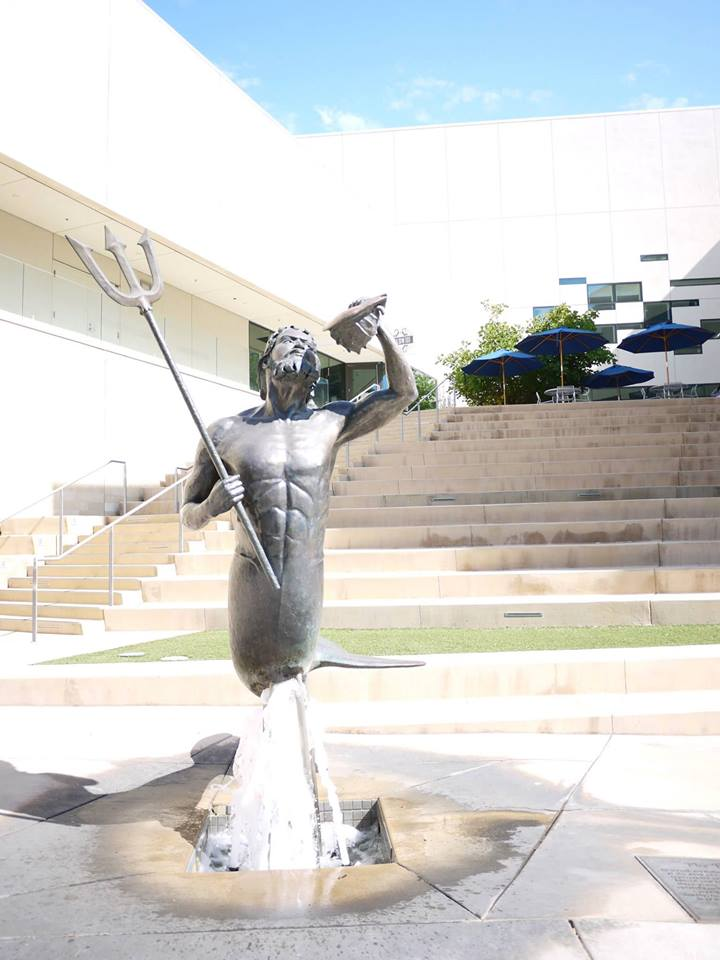
\includegraphics[width=0.45\textwidth]{Pics/tritonstatue}
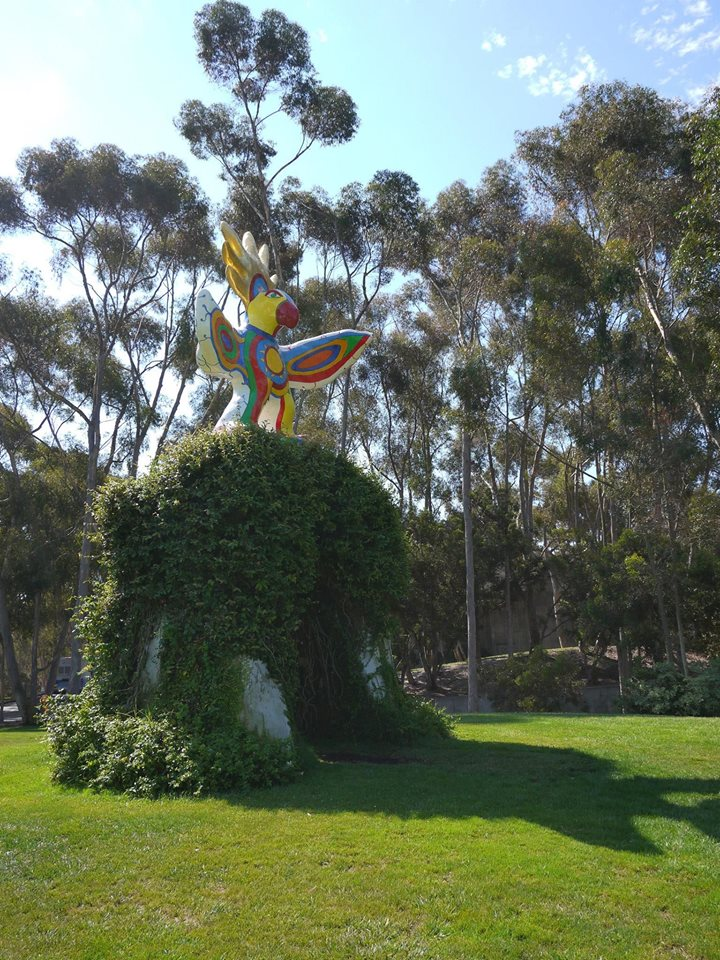
\includegraphics[width=0.45\textwidth]{Pics/sungod}
\caption{(左)UC San Diego 的精神象徵 Triton,以及(右)校園地標 Sun God。}
\end{figure}


\chapter{出國當日與入境}
\section{檢查行李}

隨身攜帶:護照(含簽證)、I-20 或 DS-2019、機票、旅支和現金、親友及接機者的電話,最好可以再次聯絡一下接機者,提醒他你的抵達時間。

申請上宿舍後,housing 會寄給你未來的宿舍地址,將宿舍地址或之後要住在哪裡的美國的住址攜帶在身邊,因為入境時會需要填到。不要忘記自己總共有幾樣行李,並且不要讓行李離開自己的視線。

\section{機場報到與登機}

一般來說要在起飛前兩小時向機場櫃台報到,或者也可以選擇在起飛前數小時前網路辦理「預辦登機」,但不論選擇哪種報到方式,都還是要在機場排隊將行李託運。行李托運前的小提醒:\textbf{注意隨身攜帶之液體、膠體皆需放在小於 100 毫升之罐裝容器中,且皆置於一個不超過 1 公升可重複密封透明塑膠袋內。}

\section{飛機上}

絕大多數的人都是坐較擁擠的經濟艙,因此如何在夾縫中讓自己得到最大舒適是一件值得大家規劃的問題。

容易暈機者,可以服用暈機藥。如果要求睡眠品質,可考慮攜帶脖枕及熱敷眼罩。有些航空公司沒有提供簡單盥洗用具,可考慮自備牙膏及牙刷。拖鞋及毛毯即使空服員沒有主動提供,也可以向空服員反應。記得某航空公司經濟艙都不主動提供拖鞋,所以如果沒拿到拖鞋可以自行向空服員詢問,原則上都應該要提供才對。

飛機上的乾冷空氣容易使人皮膚或鼻子不舒服,比較敏感者要自己注意。雖然空服員會適時提供杯水,但有時候還是很渴,一直麻煩空服員提供很多杯杯水不太好意思的話,可以考慮在進入登機室後用小銅板購買幾瓶礦泉水登機。

上了飛機後各位的留學生活就算開始了,為了應付之後一連串的美國獨立生活,在飛機上即可努力開始調整自己的生理時鐘。調整時差的方法因人而異,可以上網查詢一些空中飛人們提供的小撇步參考一下,但最重要的是選擇自己最一種最適合自己的!

因為長時間坐著,有可能會遇到水腫問題。建議上飛機穿寬鬆衣物,女生可以穿裙子並攜帶瘦身襪。偶爾在飛機上走動活動筋骨,可以事先查詢飛機上的小空間運動操讓自己無聊的時候運動一下。

對抗乾空氣的方法最簡單的就是攜帶一小瓶保濕乳液。更進階的話,可以再攜帶兩個保濕面膜及口罩。敷上面膜後戴上口罩及眼罩減緩面膜變乾的速度,敷完再厚敷保濕乳液。原則上飛機洗手間都會有基本的保濕乳液,如果懶得帶這些東西的人可以考慮去洗手間使用。

\section{填寫海關申報單}

在飛行途中空服員會開始傳遞\href{http://www.cbp.gov/travel/us-citizens/sample-declaration-form}{美國海關申報單}給旅客。海關申報單請誠實填寫\footnote{一般來說,多半勾選 no,但申報單有帶食物務必誠實申報,沒申報被查到輕則罰款了事重則留下記錄,如何處理海關自由心證;另外請避免帶非法軟體以免惹事上身。 }。攜帶金錢部分包含硬幣、貨幣、旅行支票和不記名票證,如個人支票、銀行本票、股票和債券。

必須注意的是,運送任何金額的貨幣或金融票據皆屬合法。但攜帶入/出境美國的總金額超過 10,000(美元或等值外幣總和)時,需要另外填寫 FinCEN 105 表單,並呈交此表格於海關及邊境保衛局。為了節省通關的時間,建議先行上網列印填寫\href{https://www.fincen.gov/forms/files/fin105_cmir.pdf}{ FinCEN 105 }。請將此表以雙面的方式列印,以利現場官員收件,單面列印可能會被要求現場重新填寫。

填寫完海關申報單與 FinCEN 105 後記得簽名,在通關的時候將此表與護照等文件一併給美國海關人員檢查。表上會要求填寫之後在美國居住的地址,原則上就是填入宿舍地址,如果還沒找到宿舍,可以填寫暫時居住的親友家地址或校外租屋地址

有關\href{https://i94.cbp.dhs.gov/I94/#/home}{ I-94 出入境登記表}方面,目前美國將此表設定為電子化登入,因此在入境後記得盡快登入完成並列印下來,列印的日期欄位不可以有中文(要在個人電腦上面設定,不然通常從台灣帶來的電腦都會自動將日期欄變成中文)。

\section{入境通關}

飛機落地後,再次檢查所有文件(護照、I-20 或 DS-2019、海關申報表)以及隨身行李是否都有帶著,有時候在飛機上睡得東倒西歪時,有些隨身物品就會不小心掉在地上或椅子夾縫沒有發現。

請在一可以打電話或使用機場免費 WIFI 的時候就與接機者聯絡。需要轉機的同學,發現班機有任何變動也請立刻聯絡幫忙接機的學長姐。

入境時的程序大致上為:填寫海關申報單$\rightarrow$移民官員$\rightarrow$領行李$\rightarrow$通過海關。根據學長姐的經驗,從 LAX 入境會比較費時,從 SAN 會比較迅速。

移民官員會問一些簡單問題,如就讀學校、科系、攻讀學位,學校在哪裡及之後要住在哪裡等,有時可能會問在之前是否有入境過美國,之前持有什麼簽證入境美國,在問的同時他們也會檢查你的護照、I-20 或 DS-2019,只要冷靜、誠實的回答,通常都不會有太大問題。

切記要將文件收好並在之後幾天內印出自己的 I-94,I-94 之所以重要的原因是未來出境及辦許多證件都會用到。    

移民官員還給你護照後,請當場快速確認入境章上寫的簽證種類是 F‐1(或 J‐1)以及其有效日期,若有誤請當場提出,立刻更正,真的無法現場解決,到校後請立刻到 I-Center 處理,否則之後會很麻煩。

接著就可以開心的領托運行李,然後經過海關。此時海關會\textbf{收取你的海關申報單},若攜帶入境美國的總金額超過 10,000(美元或等值外幣總和)時,請依照海關指示,前往指定區域呈交 FinCEN 105 並接受檢查;若遇抽查行李,請依照指示打開行李並照實回答海關問題即可。

\chapter{到美應辦手續}

\section{搬入宿舍}\label{sec:movein}
關於申請宿舍的程序詳見 \ref{sec:housing},在同意 housing office 的 offer 並且簽下電子合約之後,你就可以在 offer 信上指定的日期,前往各個宿舍區的 housing office 辦理入住手續。若因故必須延後入住,你可以透過電子郵件方式通知 housing office,但仍需按原先入住日期繳交租金。若你當日在 housing office 下班之前仍無法辦理入住,請以電子郵件通知 housing office,各個 housing office 會將你的宿舍鑰匙或房卡放在辦公室外的密碼鎖內,並且透過電子郵件告知密碼,請在抵達後依密碼直接取得鑰匙或房卡,待下一個上班日再前往各個 housing office 辦理入住手續。

Housing office 在你接受 offer 之後,也會將你即將入住的消息通知你的室友,並告知雙方彼此的電子郵件地址,記得在入住之前,先跟你未來的室友打聲招呼吧!

若選擇由 San Diego 機場(SAN)入境,可以事先聯絡TGSA學長姐協助接機;或是預約機場接駁專車(\href{https://www.supershuttle.com/}{SuperShuttle}、\href{http://www.primetimeshuttle.com/}{Prime Time Shuttle});抑或選擇行動叫車 app 例如 Uber/Lyft 等等。

若由 Los Angeles 機場(LAX)入境,可搭機場巴士 Flyaway 至 Union Station,車程大約半小時,車費 8 美金(到站付款,限 credit card)。抵達後再搭乘 \href{http://www.amtrak.com}{Amtrak 美國國鐵}的 Pacific Surfliner 線前往 Solana Beach Station,車程 2 小時,車費 30 美金\footnote{持用國際學生證有九折優惠,但要在乘車日(不含)3 天前上網購票。},可事先上網購票。抵達 Solana Beach 後再由 TGSA 學長姐協助接送至 UCSD。

抵達 housing office 後,入住手續要由本人出示證件證明身份(例如護照),並且簽署各項房客須知的書面同意書,部份有車位的宿舍也可以同時辦理停車證。若缺少臥房鑰匙、信箱鑰匙或需要額外的鑰匙,可在此時向 housing office 進行補發或申請,有任何問題均可當面詢問 housing office 的職員。

Housing office 在入住手續中會給你一張宿舍檢查表,以確認你入住時房間的狀況,請在到達宿舍後依照檢查表填寫房間狀況,例如牆壁有無受損,廚房、衛浴設備有無損壞等等。填寫完後繳交至 housing office,即完成搬入宿舍之程序。 

\section{購買傢俱與生活必需品}

搭乘繞行 UCSD 的週邊的 201/202 路公車可以到達 La Jolla Village Sqaure(此區有超市、簡易服飾、生活用品、電器、傢俱、腳踏車店、各類餐廳以及電影院)也可以抵達 Westfield UTC Shopping Mall。距離上,由各個宿舍徒步前往上述兩個商店區皆需花費 15 到 40 分鐘不等的時間,因此若要購買個人可攜帶之份量的生活必需品或簡單傢俱是可行的,雖然稱不上方便。鄰近 UCSD 各超市的介紹,詳見 \ref{sec:supermarket}。在 La Jolla Village Sqaure 也有量販店 Ross(衣物)、Marshall(衣物/生活用品)和 Best Buy(電器),關於 La Jolla Village Square 的這些店家,詳見 \ref{sec:shopping}。當然,在這些店家都無法滿足需求時,也可以花點運費直接上 \href{http://www.amazon.com/}{Amazon} 網路購物(新會員或是學生或有免運費的優惠,請參考Amazon網站)。

然而,入住初期需要購買大量傢俱或生活必需品,在沒有車的情況下非常不便,請聯絡有車的 TGSA 學長姊協助,到較遠的 Ikea(組合傢俱)、Costco(應有盡有)、Target (傢俱/生活用品)、Lowe's(五金/生活用品)、Home Depot(五金/傢俱/生活用品)、Office Depot(文具/辦公用品)、Walmart(五金/傢俱/生活用品) 等大型商場選購,並運回宿舍。Ikea 提供組合傢俱運送到府的服務,費用大約 60 美金。

一般而言,入住未含傢俱的宿舍,約需花費 500 至 1000 美元不等的傢俱費用,雜貨以及生活用品部份,則需花費 200 至 500 美元不等, 請準備足夠現金。如果希望節省開銷,可上 Facebook UCSD 子社團 Free or For Sale 、各宿舍區專屬子社團、或是 UCSD TGSA 社團尋找 moving sale 、二手傢俱、日用品販賣資訊。機會往往十分有限,若有需求請密切關注、回應賣方。非校內的二手購物資訊分享網站,以 \href{http://sandiego.craigslist.org/}{Craigslist} 最有名,但因為是外面的平台,請使用時特別注意資訊安全,以及交貨、付款的安全。

\section{領學生證}
UCSD 學生證將是你除了駕照之外,在校內校外最好用的身份證件,無論是圖書館借書,在系上使用影印機,上網路查詢學生資源,登記選課,都需要用到學生證。學生證還有 TritonCash 的功能,可以在校內店家當作儲值卡使用 \footnote{詳見 \url{http://tritoncash.ucsd.edu/}。}。

欲領取學生證,請至 University Center 的 Student Service Complex ( Price Center 前面一棟5層樓高的現代建築)三樓 Student Business Services 辦理。領取時記得攜帶護照或其他身分文件。若現場服務人員找不到你的證件,則可能是被所屬系辦人員領取了,請再與系上聯繫。

\begin{figure}
\centering
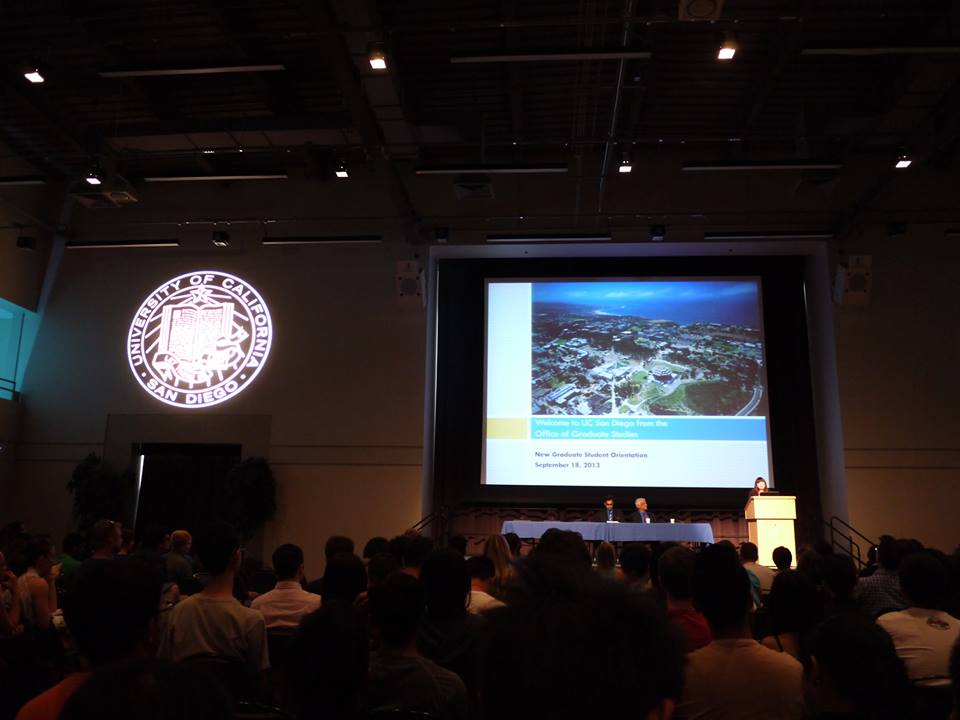
\includegraphics[width=0.5\textwidth]{Pics/orientation}
\caption{Graduate student orientation 現場。}
\end{figure}

學校大約會在七月時向您索取個人照片供學生證使用,若您沒有提供,則學生證上的照片將會是在領證時現場拍照。若你會介意的話,請整理好服裝儀容後再領證,以免拿到證件時後悔莫及。

Bus sticker請注意開放領取的時間和地點,要先繳交學費才可領取,有sticker即可免費搭乘shuttle bus和大部分MTS。MTS 經過 UCSD 的巴士以及trolley皆可憑貼紙免費搭乘。若是住在 Mesa 及 OMS 宿舍區的同學平日可以搭乘校園巴士 M 線 Mesa Shuttle 往返學校及宿舍。

\begin{figure}
\centering
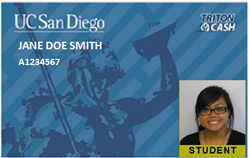
\includegraphics[width=0.4\textwidth]{Pics/studentid}
\caption{UC San Diego 學生證樣張。圖片引自:\url{https://students.ucsd.edu/finances/campus-cards/}}
\end{figure}


\section{網路與門號申辦}

校內 wifi 有兩個入口,剛到學校還未註冊請用 UCSD-GUEST ,開啟瀏覽按指示登錄即可,註冊後可使用 UCSD-PROTECTED,帳號密碼跟學校的信箱是一樣的(帳號是姓名縮寫+數字的那組)。

南加州主要的電信公司有 AT\&T、T-Mobile、Verizon,三家電信公司都在學校附近(開車 5 至 10 分鐘)設有門市,其中以 AT\&T(在 La Jolla Village Square 有店面)和 Verizon 訊號狀況較佳。新生組團申辦手機,可選擇加入 family plan 或 share plan ,舉例而言(僅供參考,實際狀況異動頻繁,請詢問學長姊與電信公司), family plan 可能為 3 至 5 人的團體一起申辦手機,每月支付固定基本費率(50 至 100 美元不等)服務項目可能包含無限制網內互打、簡訊、以及多人共享單月固定 4G 網路流量(1 GB 至 10 GB 不等),當網路流量超過單月共享量,或播打網外長途、國際電話時,增加個別使用者之費率。

另外網路用量如果不大的話,也可以考慮AT\&T的子公司Cricket。覆蓋範圍幾乎跟AT\&T一樣,可以用AT\&T的全部信號台,只是不能用合作企業的信號台。Cricket只要購買好買預付卡,就可以在網路上進行各種操作(選Plan等等)。

無論 share plan 或 family plan,會需其中一人擔任「家長」或「負責人」,除此之外,綁約之初需繳交保證金(價位約在上百美元的數量級),約滿後退費。Cricket則是因為都是用預付卡形式,家長不需要繳保證金。

請特別留意,\textbf{美國通話費、簡訊費,皆為收發方雙邊付費}(但通常很多plan都是unlimited call and text,可以仔細看看選擇)。

\section{銀行開戶與與信用紀錄}\label{sec:banking}
\subsection{銀行開戶}
銀行戶頭依其功用而言一般分為 checking account (支票帳戶)和 saving account (儲蓄帳戶)兩種類型,checking account 為直接連接 debit card (類似郵局現金卡)的帳戶\footnote{也有某些銀行可用 debit card 提取 saving account 的存款。},也是使用支票、電子支票的扣款來源,總括來說,是所有金額匯入匯出的帳戶,具有利率低(甚至零利率)但存提款次數、方法幾乎無限制的特色。相對地, saving account 具有較高的利率,但通常無法連接 debit card 直接使用,也無法用此帳戶開立支票、電子支票等等。同時,saving account 可能會有特定的存款、提款次數限制(例如單月轉帳六次以下),若超過此限制則需額外手續費等等。以學生的需求,通常兩種帳戶皆需開立一個。

值得注意的是,checking account 以及 saving account 在帳戶內存款不足的情況下皆有可能需要定期向銀行繳交管理費,詳情請在申辦時仔細詢問銀行職員,並詳閱申辦合約。

在南加州生活,各種購物消費,小至食物、大至學費、購車,多半可使用 debit card 或 credit card (信用卡)付費,其中 credit card 需要足夠優良的「信用紀錄」才能夠申辦成功(剛到美國時可以考慮信用紀錄門檻較低的 credit card ,或是 secured credit card\footnote{secured credit card 的運作方式是申辦後先 deposit \$500--1000,這初始金額會變成申請人每月的 credit line,可累積信用點數。一般過半年後就可以申請真正的信用卡了。})。Debit card 則不用信用紀錄,只是一種使用帳戶內存款來消費的方法而已。除此之外,學校線上付費系統往往透過電子支票 eCheck 付費(詳見 \ref{sec:tuition}),同時,你也有可能會遇到某些時候,不得不透過支票來遠距郵寄款項(例如在外地繳交房租)。上述的各種使用情形,皆需用到銀行的服務,因此到銀行開戶並申辦 debit card 是絕對必須的。

UCSD 校內唯一的銀行是 Price Center 內的 JPMorgan \& Chase 分行,有華裔專員可以用中文溝通、開戶。鄰近 UCSD 的主要銀行分行有 Bank of America、Wells Fargo、Citibank,其中除了Citibank 之外在校內皆有自動櫃員機可供使用。

至銀行辦理開戶需要以下證件:護照、I-20、第二證件(如學生證、駕照等等),如果在開戶時已經拿到 social security number,也應攜帶。國際學生至銀行開戶需要填寫 W-8BEN 表,可使利息免稅,不然報稅時會比較麻煩。\href{http://www.irs.gov}{美國國家稅務局網站}有此表的檔案可供下載參閱。

部分銀行不定期會釋出開戶 bonus coupon ,建議新生在開戶前可多上網留意。

\subsection{信用紀錄}
對於有 TA 、 RA Offer拿到SSN的人來說,可以考慮申辦信用卡,以利開始建立自己的信用紀錄。美國不少信用卡有不錯的現金回饋、點數回饋或開卡禮,若對這些有興趣的建議從到美國開始就找人討論,並留意自己的信用紀錄。

信用紀錄會綁定個人的 SSN ,其意涵為「這個人借錢還錢的紀錄」,會影響到辦理信用卡成功率、信用卡的Credit line(消費上限)、各類貸款的上限以及利率等,對於想要長期在美國生活的人來說可謂重要。

提升信用分數的常見方法如下:
\begin{enumerate}
\item 按時償還貸款。
\item 按時繳交信用卡費,並控制每個月 statement 上的花費與 credit line 的比例。
\item 提高手上信用卡的 credit line 總合,方法包含提升已持有卡片的 credit line 和申請新卡。請注意,每次申請新卡與申請 credit line increase 都可能在你的信用紀錄留下一個為期兩年的 hard pull 紀錄,降低信用分數。
\item Credit History 越長越好。
\end{enumerate}

\section{I-Center 報到並參加說明會}
到達學校後請盡快至 International Center 報到,需要攜帶的文件有: 含 F-1/J-1 簽證的護照, I-94, I-20, DS-2019。 I-Center 地點位於 Mandeville Ln 及 Library Walk 之間。

學校規定國際學生皆必須參加 I-Center 舉辦之說明會,請至 I-Center 網站報名場次並參加說明會。

\section{系上報到}
系上報到依各系所要求而異,建議注意個人信箱有無相關訊息,或向本科系/相關科系的學長姐做確認。目前學校要求領取學生證時需要系上的證明文件,故須先至系辦領取相關文件;亦有科系的系辦人員會提早將新生的學生證領回系上,由系上統一發放。

對於有 TA、RA 身分的留學生,到系上的人事部門報到是必要的,因為系上必須建立你在 UCSD 的職員資料,並要求你簽署相關文件。另外,申請 SSN 的信函也須先向系上領取,才能跑 I-Center。

\section{繳學費}\label{sec:tuition}
繳學費有兩種方法,到 cashier 現場繳或是用 \href{https://act.ucsd.edu/myTritonlink20/display.htm}{TritonLink} 線上繳:
\begin{enumerate}
\item Cashier:位在 Student service center 的一樓,基本上學校要繳的費用都可以在這邊繳。但要注意的是這邊不收 debit card 或 credit card ,只收 cash、personal check (個人支票)、 traveler's check (旅行支票)、 money order (匯票)或 cashier's checks(銀行本票),所有項目都必須以 US Dollars 為單位。
\item TritonLink:當有了 PID,可以登入 TritonLink 之後,點選 Financial tool $\rightarrow$ Billing \& Payment 進入頁面後,再點選 View or Pay Bill,可以看到目前尚未付款的總額。一般我們是用 eCheck(有50 cents的手續費) 來付款,在頁面中點選 Pay Total Current Balance,再來照著指示做,就可以付學費了。TritonLink 現在也可以用信用卡付款,不過會收取接近 3\% 的手續費,通常不建議使用。另外要從台灣付款也可以透過與 TritonLink 合作的 Western Union,不過這是透過海外匯款的方式,過程較繁瑣而且需要較多工作天。\footnote{TritonLink 付款一定要付欠款的總額,舉例來說,假如現在必須付給學校學費加房租,則用 TritonLink 就只能一次全部付清。如果想要分開付的話必須要去 cashier。}。
\end{enumerate}

\section{考駕照}
考駕照分為筆試跟路考,都需要在 DMV(Department of Motor Vehicle)進行,離學校最近的 DMV 是 Clairemont DMV 以及 Poway DMV。整個流程可以參考\href{https://www.facebook.com/groups/13591139149/10151810813429150/}{這篇連結文章}\footnote{感謝 Hung-Wei Tseng 學長、Chun-Tse Shao 學長和 Conway Wang 學長},還有附件的 Powerpoint 投影片。

\subsection{考筆試}
需要帶的東西:護照、I-20、I-94 紙本、兩份居住證明以及 33 元考筆試費或 debit card(不收 credit card )。如果提前預約的話會節省一點時間,不過還是要有心理準備可能要花上半天到一天的時間。

考試可以選擇中文版,建議先熟做\href{http://www.ccyp.com/TRAFFIC/}{考古題},考試時最多可以錯六題。

考完筆試之後會拿到教學駕照(learning/instruction permit)。Learning permit 有效期限為一年,但規定在開車時,副駕駛座必須要有駕照的人隨行,所以在考路考的時候,必須要找一位有駕照的人同行。

考筆試可以先到 dmv 網頁上預約,或是現場排。若是當天現場排建議可以一大早就出門。

\subsection{路考}
首先考路考之前必須要預約 behind-the wheel driving test,可線上預約也可以到 DMV 現場預約,考完筆試也可以直接預約路考時間。預約後在 Clairemont DMV 一般都要等兩個禮拜才能考,等待時間為兩個小時左右。

在考試之前,建議要找一位個考過駕照的人仔細帶你練車,將考試路線練熟再上場,會對考試非常有幫助。

\section{買車(新車、二手車)、保險}
在買車之前,你要估計所有買車加養車要花的預算有:買車的錢(未稅價格 + 稅 + DMV註冊費,全部合稱 out-the-door (OTD) price)+ 保險費 + 保養費 + 油錢 + registration renew fee。

\subsection{買新車}
買新車,基本上品質都有一定的保證,也不太需要考慮車況的問題,所以買新車主要是以談價錢為主。價錢可以參考各大查價網站 (\href{http://www.kbb.com}{KBB}, \href{www.truecar.com}{Truecar}),可以查到價錢有兩個:factory invoice 跟 MSRP (manufacturer's suggested retail price)。

Factory invoice 指的是 dealer 拿到車子的均價,而 MSRP 指的是 dealer 賣給客戶的均價,一般來說,價錢都可以談到含稅之後的 outdoor price 可以跟 factory invoice 差不多。

另外 TGSA 很多對買車談價錢很有經驗的學長姐,可以幫助你拿到好價錢,別忘了多多找尋學長姐的幫忙!

最後,買新車的好處就是所有的事情 dealer 都會幫你辦到好,包括去 DMV 註冊的程序。

\subsection{買二手車}
買二手車又可以分為跟 dealer 買,或是 private party。買二手車最基本要注意的就是:廠牌、車型、年份跟里程數。當然還有許多細節要注意,但是這幾項最基本的絕對是買二手車前最需要注意的幾個地方。

\begin{enumerate}
\item Dealer--跟 dealer 買有跟新車一樣辦到好的好處,不過在買的時候需要注意以下幾點:
    \begin{enumerate}
    \item 要注意車子有沒有 certificate,有的話代表不是事故車。另外你可以跟 dealer 要這輛車的來源,還有他所有的歷史記錄,有些車可能是由租車公司賣出,在車況上會比較有疑慮。
    \item 一般來說,美國車主平均的里程數是 12000 miles/year,如果里程數過高就要特別注意。
    \item 試車建議找要有經驗的人幫忙。仔細聽引擎聲是否有不正常,還有車開起來是否平穩。
    \item 關於價錢除了一樣上各大查價網站查價之外,也可以比較多家 dealer 開出來的價錢,多做功課知道價錢的 range 大概在哪裡。然後談價時可以多帶幾個人去,有耐心堅持底價就可以拿到好價錢。
    \item 關於價錢部分網站上提供的價錢絕大多數是未稅價格。但一般來說買車的費用為:未稅價格 + 稅 + DMV 註冊費\footnote{車子每年須註冊一次。在車子後方的車牌會貼有上次註冊的有效年月,在該日期前必須重新註冊。買二手車時,若該車已屆須註冊日期,須特別向 dealer 確認註冊費是由買方或賣方出。}。 因此許多人在談價錢的時候是談所謂的 ``out-the-door price'',即是你最後付給 dealer 的價錢是未稅價格 + 稅 + DMV 註冊費。在跟 dealer 談價錢的時候一定要特別留意。
    \item 跟 dealer 確定他們能提供,除了原廠以外的額外保固是多久。
    \end{enumerate}
\item Private party--跟 private party 買,因為原車主通常不會幫車子做 certificate,所以價錢比較低,也更容易買到事故車。在選擇時建議跟對方確定賣車原因,篩選出原因較正常的,例如要回國的學長姐。價錢方面一樣要參考各大查價網站,另外由於做 smog(交車前的檢查),還有去 DMV 辦交車都要額外付錢,所以雙方也要先談好這些額外的錢要由誰付,以免不歡而散。
\end{enumerate}

\subsection{保險}
汽車保險很重要,法律規定一定要保險才可以開車上路。建議在買車前就上網先向多家保險公司要 price quotation 比價,並留下業務聯絡資料,買車當日確認車子的 VIN(Vehicle Identification Number)再和業務定案。強烈建議不管車輛還是保險,都和有車的學長姐討論過後再出手。通常一次付清半年、一年的保費會比月繳來的便宜。

汽車保險又分為以下細項:
\begin{itemize}
\item Bodily: 事故後,賠「別人」的「人身傷害」的 單人/整起事故 最高額度。加州法律規定必保,下限15k/30k。
\item Property: 事故後,賠「別人」的「財物損失」的最高額度。加州法律規定必保,下限10k。
\item Medical: 事故後,專賠「醫療」的支出。
\item Uninsured Motorist (UM): 事故後,若對方駕駛/騎士沒有保險而我方有保險,法律規定我方保險公司要幫忙對方出錢。UM就是用來對付這種奇怪的情況。
\item Comprehensive & Collision: 兩者都是「修自己的車」,且deductible金額X代表「若修車費用Y $>$ X,保險公司幫你出Y-X;若Y$<$X,則保險公司不負責」。通常新車都會保(而且保費頗高),舊車不一定。Comprehensive則是賠償所有不是因Collision造成的損傷。\footnote{若有標註"deductible"代表若是在事故中損傷,且事故責任在對方,則可以減免金額。}
\item Rental Reimbursement: 補強被保人租車時的保險。
\item Emergency Road Service (ERS): 道路救援服務。
\item Mechanical Breakdown Insurance (MBI): 任何原因造成的車內電器損傷維修(例:air conditioner)。金額詮釋同Comp./Coll.。
\end{itemize}

在買車時,只要是跟 dealer 買的,他們通常都會有自己合作的 insurance company,而且都是大公司,通常就直接跟他們保就可以了\footnote{但還是有可能被坑,要先自行聯絡或請dealer幫忙見仁見智。},你可以向他們要求 discount,只要你符合資格的,例如好學生折扣,他們通常都會幫你辦到好。另外至少要temporary driver license才能買車,而且保險費會不一樣,還沒過路考會稍微貴一些。

如果是和 private party 買的話,則保險要在買之前就先行辦好,只要上路,就必須要有保險證明,DMV 交車的時候一樣也要看保險證明。建議買車前先向各大保險公司(如 State Farm, Geico, USAA, Farmers 等)要 quotation,這樣可以先比價。如果要買新車,甚至可以直接給保險公司車子的型號直接買保險,可以省去殺完價買車之後還要談保險的時間。

另外,若在台灣監理所先申請「無肇事証明」,可以省一些保險費。

\section{腳踏車}

由於學校平日停車需要購買 permit,找車位又是一大麻煩,除了公車之外,腳踏車也是一個非常方便的選擇,從 OMS/Mesa Nueva 宿舍騎腳踏車到學校 Price Center 途經宿舍區北邊醫院費時約 15 分鐘以內,學校對騎乘腳踏車者也有一些福利和優惠,例如每個 quarter 10 天免費校內停車、腳踏車店折扣、免 zipcar (自助租車)註冊費等等,因此若是購買全新或是二手腳踏車,別忘了至學校註冊以享有這些優惠,詳細內容以及申請流程請見學校網站\href{http://transportation.ucsd.edu/alternatives/cycling/pedal.html}{連結}。

在美國騎乘腳踏車也請注意道路規則,例如在 stop sign 必須停車、學校 library walk 禁止騎車等等,另外學校也提供安全帽補助,詳細內容請\href{http://transportation.ucsd.edu/alternatives/cycling/index.html#UC-San-Diego}{點此}。

\section{辦社會安全碼}
如果有拿到 TA/RA、fellowship、校內打工、實習等等會要領薪水的人,就會需要辦理社會安全碼 (social security number,簡稱 SSN)。SSN 相關資訊可以在 I-Center 的\href{https://ispo.ucsd.edu/current-students/working-in-usa/social-security.html}{網站}上取得,以下為 申請SSN所需流程:
\begin{enumerate}
\item 拿到I-Center的Letter from UCSD
	\begin{itemize}
	\item 必備物品:Department 給的 offer letter (當初錄取時系上給的。沒有的話請洽系辦)。
	\item 地點:I-Center @ UCSD。
	\item 時間:到 I-Center 報到時就順便問能否申請了。平常日09:00~16:00。
	\item 過程:
	\begin{enumerate}
		\item 走到櫃台,說你想申請SSN,出示 offer letter。
		\item 櫃台人員會給你一張申請表,並且copy你的 offer letter。
		\item 填完表後交出。預計五個工作天後可拿到 Letter from UCSD。可以領取時會 e-mail 通知。
	\end{enumerate}
	\end{itemize}
\item 拿到 department 的聘僱證明(可與1.同步進行),地點、過程請洽各系辦。
\item 申請 SSN
	\begin{itemize}
	\item 必備物品:
	\begin{enumerate}
		\item 證件類:Passport、I-20\footnote{持 J-1 簽證身份的交換學生,則改為攜帶有效的 DS-2019 表單}、I-94。
		\item \href{http://www.ssa.gov/forms/ss-5.pdf}{Application form }填完印出來 (page 5)。
		\item 1.拿到的Letter from UCSD和2.拿到的聘僱證明
	\end{enumerate}
	\item 地點: Social Security Administration (SSA) @ Downtown San Diego。
	\item 時間:入境美國10天後。平常日09:00~15:00,週二只開到12:00。
	\end{itemize}
\end{enumerate}

跟系上取得文件後(以防萬一也請順便帶上 official 的 UCSD 錄取信、UCSD 學生證),可以從學校搭 150 到 San Diego downtown 的 SSA進行申請,但是 150 到市中心的車程路遙遙\footnote{150 從 UCSD 到 Downtown Social Security Office 附近約 30 分,回程則在隔壁街上車,可上 Google Map 或 \href{http://www.sdmts.com/}{SDMTS 網站} 查詢路線和時刻。},如果可以請人開車載去會省下非常多時間。進去 SSN office之後,抽號碼牌,領 SS-5 表格並填入資料(此表格可以上網列印先填,也可到現場再拿)等待時間通常會長達四十分鐘到一個半小時。通常只要文件備齊,記得自己爸媽英文姓名拼音、自己的基本資料等等,在 officer 問問題時誠懇的據實回答,通常都會通過。如果 officer 確認受理你的申請,會給你一份收據,請記得保存好。卡片通常會在一周到一個月內寄到家裡\footnote{2014年工作人員都是說兩週內寄到,而實際上大多四個工作天收到。},超過一個月沒有領到的話請親自(打電話沒有用)儘快跑一趟 SSN office (今年就有人等待長達三個月都還沒有收到 SSN 卡)將當初申請時候的資料一起帶上,告知他們你已經申請超過一個月,officer 會幫你進行確認。

\chapter{在美生活}

\begin{figure}
\centering
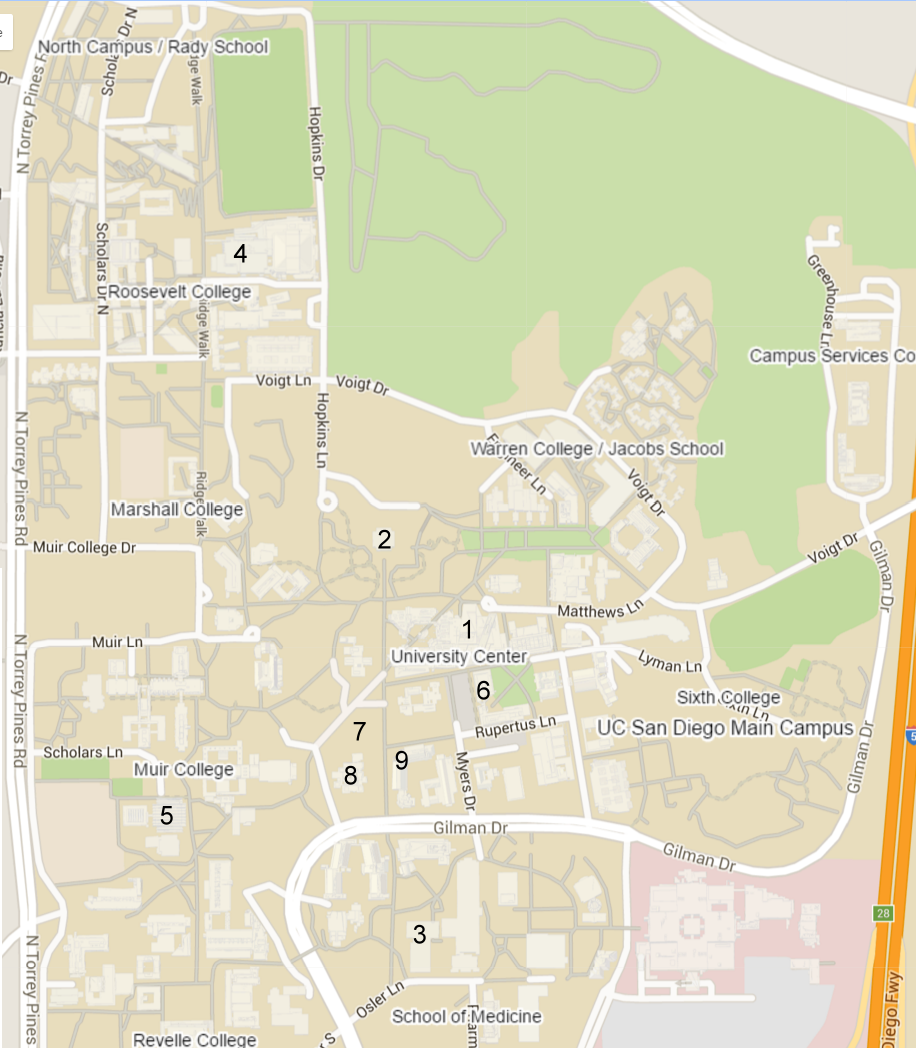
\includegraphics[width=0.6\textwidth]{Pics/map}
\caption{學校幾個常見地點} \label{fig:map}
\end{figure}

\section{學校常見地點介紹}
UCSD的校園雖然大,但常去的地點也不會說太多,大多都集中在Gilman Drive \& Myers Drive附近。下面列出的點所對應的地理位置可以參考圖\ref{fig:map}。工學院的位置在Warren College / Jacobs School,管理學院則是在地圖左上方的North Campus / Rady School。

\begin{enumerate}
\item Price Center:有各式的餐廳,咖啡廳,Sunshine Market(小超市),bookstore
(其實什麼都賣),和Chase銀行。

\item Geisel Library:大學部的圖書館,內有多人\href{http://libraries.ucsd.edu/spaces/reserve/}{ group study room }可以上網借。

\item Biomedical Library:研究所的圖書館,一般研究生比較常去這個圖書館,內也有多人group study room可以借,連結跟上面的一樣。 

\item RIMAC:校內最大的健身房。

\item Main Gym and Rec Gym:各類球類運動,內也有健身房但設備沒有RIMAC多。

\item Student Services Center:拿學生證的地方(
3樓Student Business Services),另外Graduate Division和Cashiers Office也在此。

\item Career Services Center:可以\href{https://career.ucsd.edu/individual-advising.html}{預約}一對一改履歷,不過因為很搶手,記得早點約。

\item International Center:跟國際學生相關的事務。

\item Center Hall:很多課的教室所在地。
\end{enumerate}

校方有提供線上的\href{http://act.ucsd.edu/maps/}{地圖},可以輸入地點查詢所在位置與提供兩地路線建議。我們有將一些常見地點標示在\href{http://act.ucsd.edu/maps/?lat=32.881&lng=-117.2305&t=roadmap&z=15&p=8101341227612288%2C647%2C1431339068347577%2C525%2C440%2C438%2C436%2C526%2C7001220390468232%2C632%2C514%2C2111241524552318&r=100&v=3
}{此地圖}上,可以點選Marked查看。

\section{公車常見路線介紹}
學校附近要搭公車去買菜、逛mall或者去海邊還算方便。搭一次公車\$2.25,如果是express則是\$2.50(express停比較少站,也比較少見)。建議剛來可以先買一張\href{http://www.sdmts.com/fares-passes/compass-card}{ compass card},搭公車會比較方便,不用準備零錢。另外,繳交學費後,大概開學前一週可以在學校拿到 bus sticker 貼在學生證上,搭公車出示貼紙就可以免費搭乘。
以下列出幾個常搭的公車路線,都有到學校 Gilman \& Myer 站(括號內是站名)。

\begin{enumerate}
\item 201/202:
\begin{enumerate}
    \item Ralphs, Trader Joe's, Wholefood超市,CVS,AT\&T,La Jolla Village Square 一帶 (Nobel Dr \& La Jolla Village Square Drwy)
    \item Vons 超市 (Arriba St \& Regents Rd)
    \item UTC mall (UTC Transit Center)
\end{enumerate}

一般從校外到學校會搭202公車,從學校到校外則是搭201公車,兩台公車開的方向相反。

\item 41:
\begin{enumerate}
    \item 去Clairemont DMV考駕照筆試(從學校往 Fashion Valley 方向搭,在 Genesee Av \& Derrick Dr下車)
    \item UTC mall (Genesee Av \& Nobel Dr)
    \item Fashion Valley Mall (搭到底站Fashion Valley Transit Center)
\end{enumerate}

\item 30:\\
UTC、Coast Apartments(La Jolla Shores Dr \& Horizon Way)、La Jolla Cove(Torrey Pines Rd \& Prospect St)、Pacific Beach 到 Old Town和Downtown


\item 150:Downtown express\\
如果要去 old town 或者 downtown 可以搭 150,停的站比較少,也比較快。如果想要自己搭車去ikea,可以搭到 old town 然後轉 Green Line trolley(電車)往 Santee 到 Fenton Parkway Station。

\item 236:Mira Mesa express,可以搭到Mira Mesa的大創與韓超H Mart。

\end{enumerate}

\section{校車介紹}
校車路線圖可以參考
\href{https://www.ucsdbus.com/map}{UCSD School Shuttle Map},點選右邊的線路就會看到該線路的行經範圍。
一般來說最多人搭的兩個路線為 Mesa Housing Shuttle 與 City Shuttle。Mesa Shuttle有經過 Mesa 宿舍與 One Miramar Street (OMS)宿舍區。
City Shuttle則是經過許多鄰近學校的校外住宿區。Mesa shuttle不檢查學生證、City shuttle上車地點若在校外,司機會檢查學生證。
校方也有提供\href{http://www.ucsdbus.com/map}{互動地圖},方便大家比較各路線。

UCSD App 介紹:
UCSD有為學生製作隨身APP,方便學生從其中得到即時資訊,其中最廣為人知的就是校車即時追蹤功能。

\begin{figure}
\centering
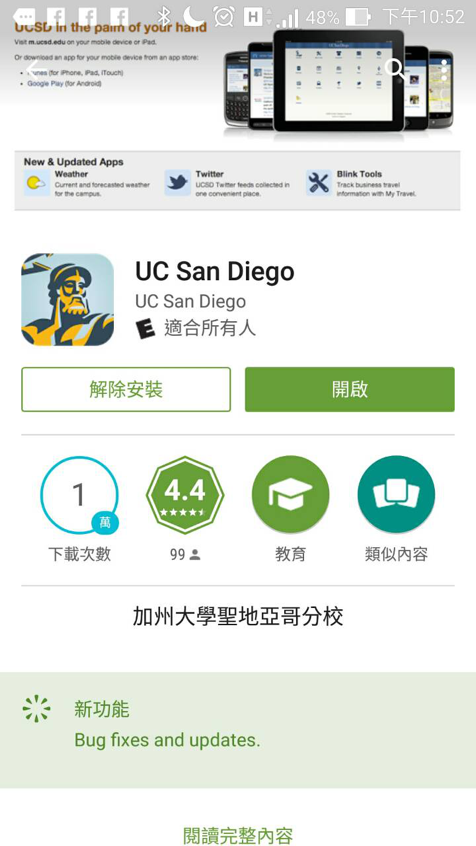
\includegraphics[width=0.25\textwidth]{Pics/shuttle_1}
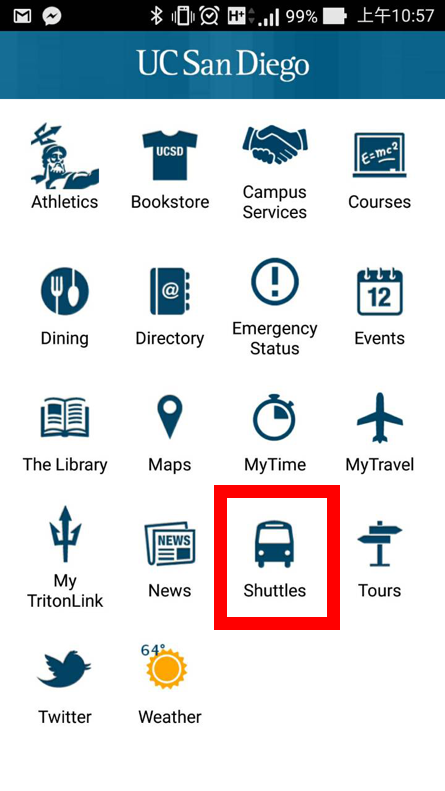
\includegraphics[width=0.25\textwidth]{Pics/shuttle_2}
\caption{左圖為UCSD app Google play的下載頁面(也有iOS版本),右圖為app的介面,紅框為常用的校車追蹤功能。
}
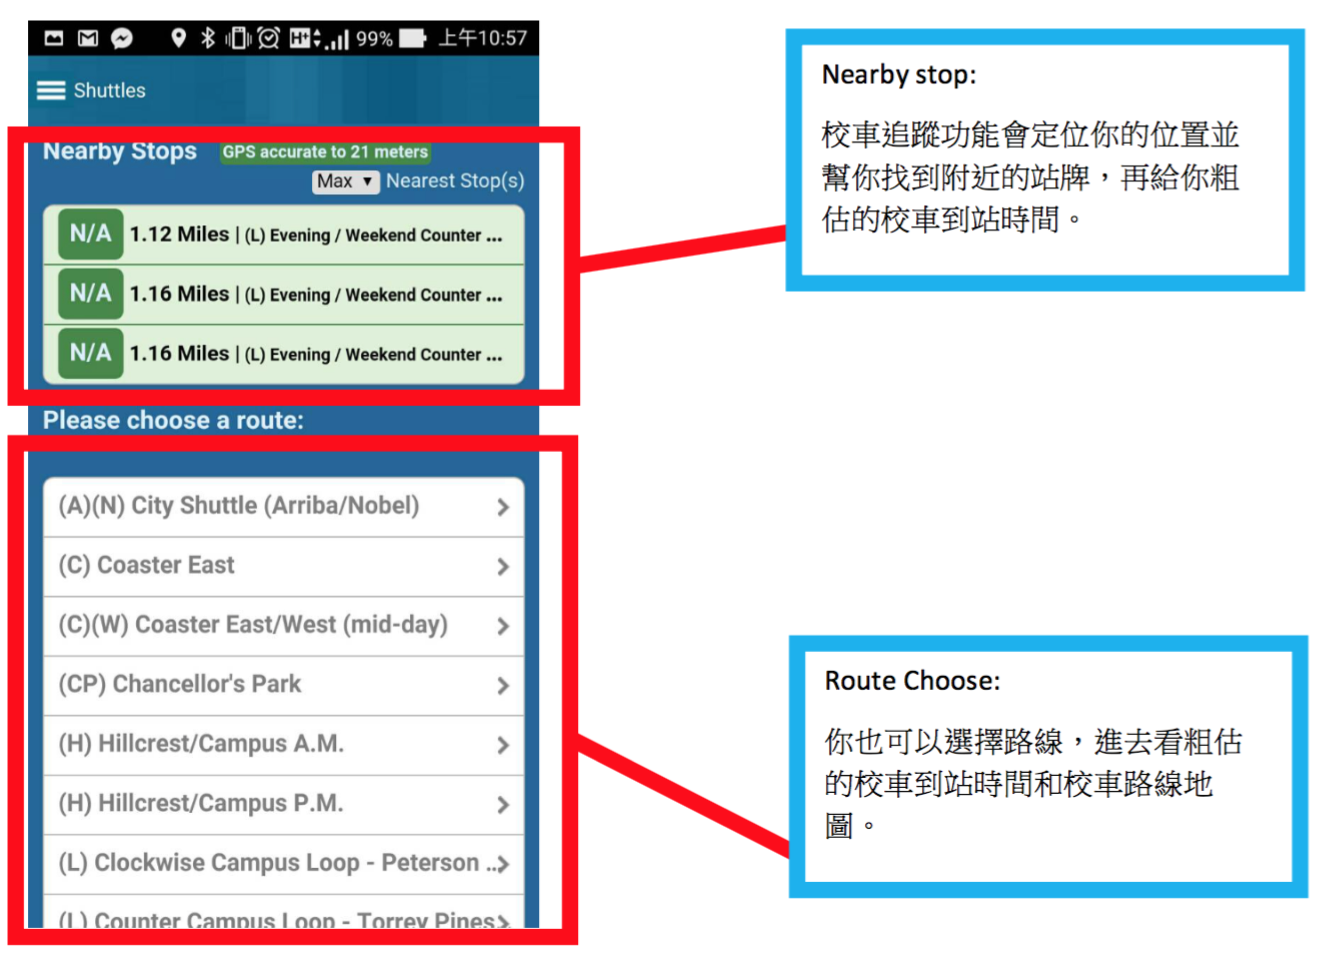
\includegraphics[width=0.6\textwidth]{Pics/shuttle_3}
\caption{校車追蹤功能介紹之1} \label{fig:shuttle_3}
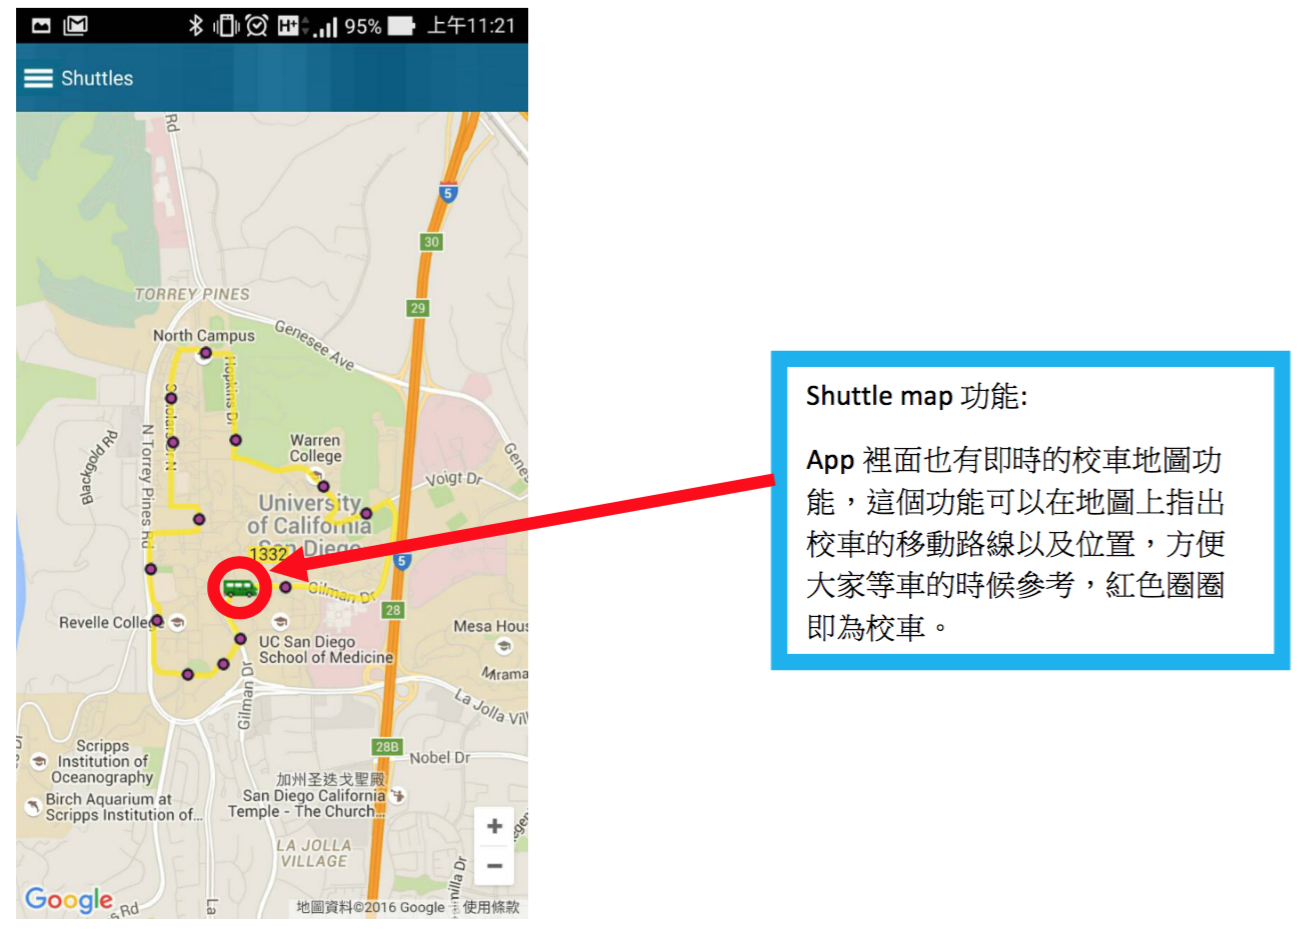
\includegraphics[width=0.6\textwidth]{Pics/shuttle_4}
\caption{校車追蹤功能介紹之2} \label{fig:shuttle_4}
\end{figure}

校車追蹤功能介紹請參考圖\ref{fig:shuttle_3}與圖\ref{fig:shuttle_4}。

\section{超市}
\label{sec:supermarket}
相關地圖請參考此 \href{https://mapsengine.google.com/map/edit?mid=zQtEEXrWDims.k7LCNq-XBdbU}{Google Map}。

\begin{enumerate}
\item 美國超市。美國超市基本上東西算是蠻齊全的,生鮮食品、蛋乳製品、飲料零食或水果應有盡有,以下三家常見又在學校附近的超市

\begin{enumerate}
\item Ralphs/Vons:價格最平民,相較其他兩家超市有較多的生活用品。(Ralphs 在 La Jolla Village Square、Vons 在 La Jolla Del Sol 南邊。)
\item Trader Joe's:價格中等,標榜有機食材。有大量的自有品牌的冷凍食品、微波食品、食物半成品。(Trader Joe's 在 La Jolla Village Square。)
\item Whole Foods: 價格最高,也是標榜有機食材,超市內有熟食區,秤重計費的自助吧,一餐約 10--15元。(在 La Jolla Village Square。)
\end{enumerate}

以上超市都在學校附近,剛來人生地不熟可以先靠它們存活下來,可從學校搭 201 坐到 La Jolla Village Dr. 站,若住 Mesa 或 OMS 可先搭shuttle 到學校再轉搭 201,住 Coast 搭 30 號公車,Rita 走路就可以抵達,SGA 也是從學校搭 201。如果只是要去Vons住Mesa的人也可考慮用走的(比Ralphs近)。

\item 亞洲超市。東西也都很齊全,生鮮、蔬果、零食或生活用品樣樣都有,每間都有自己的民族特色,以下幾家亞洲超市都在 Convoy Street 和 Clairemont Mesa Boulevard 路口一帶,要開車才能抵達。請多多抱緊有車的大腿或學長姐,在這些地方買東西是省錢的最佳手段。

\begin{enumerate}
\item 華人超市(大華 Ranch 99):顧名思義擁有非常多的華人食材,一走進去就有很熟悉的感覺,醬油、醋、各種香料都可以在這邊找到,有塊在賣各部分的溫體豬肉,比起其他被雞牛充斥的超市算是一大特色。但是這裡的豬肉味道較腥,建議須要跑活水或者先煮或者醃過再調理,追求以迅速簡單烹煮豬肉者可考慮到其他亞洲超市購買。

\item 韓超(Zion):有許多韓國特色的東西像是泡菜、有陣子很紅的香蕉牛奶、又甜又會噴汁的韓國新高梨,最特別是有區在賣已經醃好的肉和火鍋用肉片,若要 BBQ 的話來 Zion 非常的方便。Zion 同時擁有這幾家店裡面最便宜的蔬菜(像是超便宜的菠菜、打折時很便宜的蔥)。此外,韓國超市外面有一家精緻的韓國麵包店,麵包跟蛋糕都非常精緻好吃,相當推薦買完菜之後順路逛逛。

\item 日超(Mitsuwa):Mitsuwa 為 San Diego 三間日本超市中價位最低的一家,但相對也較多商品非日本製。日本超市的肉類與蔬菜在所有超市中品質最好,肉類尤其新鮮,當然價錢同樣也比其他超市略貴了一些。在這裡也可以買到各式日式食物、點心、茶飲、調味料,超市中也有販售便當(晚上7點後打折)、炸雞、可麗餅與生魚片,是帶便當的好幫手。Mitsuwa 店外有一家山頭火拉麵,口味跟日本當地的山頭火幾乎一樣,山頭火隔壁有一間日本丼飯---茅場,同樣非常好吃。
\end{enumerate}
\end{enumerate}

\section{校內飲食}

\begin{enumerate}
\item Price Center(簡稱 PC):最多人吃飯的地方,各種餐廳都有,中式的 Panda Express 和 Tapioca Express(有賣珍奶跟鹽酥雞)、日式的 Shogun、希臘式的 Santorini Greek Island Grill、印度風的 Bombay Coast、美式的漢堡王、 Subway、義式的 Round Table Pizza、咖啡店Perk、果汁店 Jumba Juice 以及小超市 Sunshine Market。中午大部份的研究生都聚在這吃飯,看到學長姐別害羞,快坐下來一起聊聊天吧。如果要帶便當的話,Price Center 有公用微波爐可以加熱食物。

小訣竅:這邊的漢堡王幾乎是最便宜的店,購買前請先下載漢堡王App,你會發現新天地。

\begin{figure}
\centering
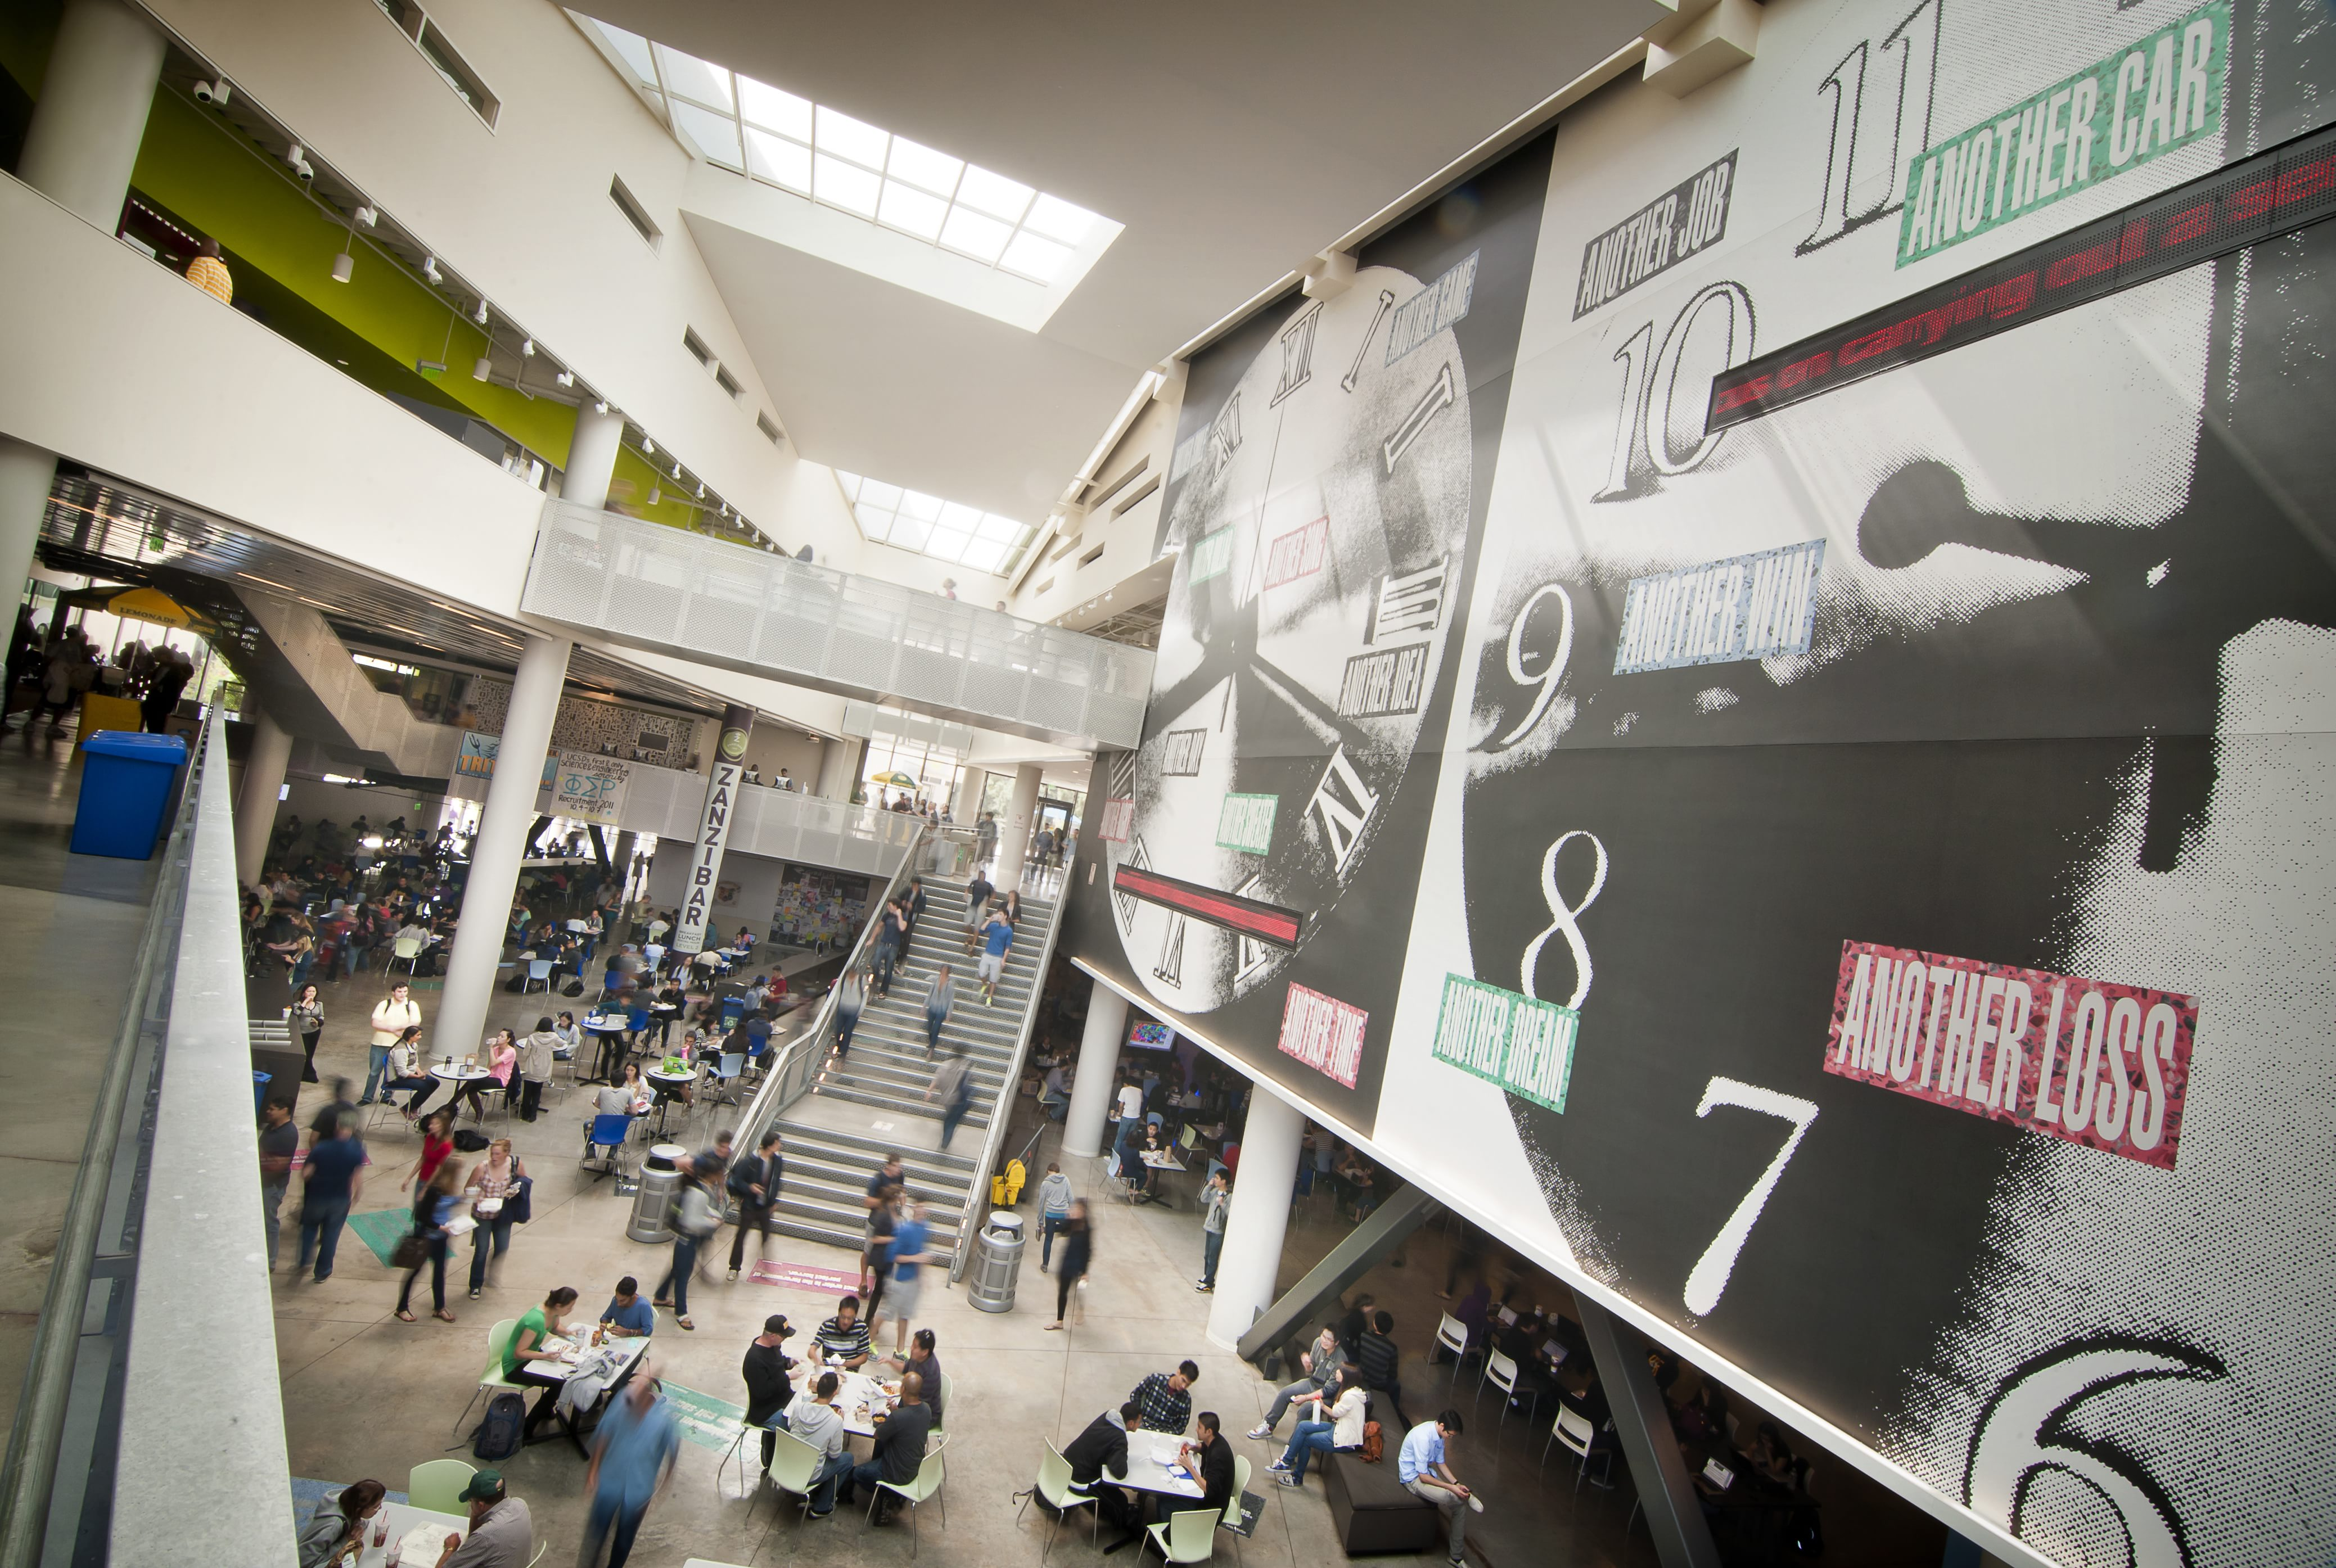
\includegraphics[width=0.47\textwidth]{Pics/pc-min}
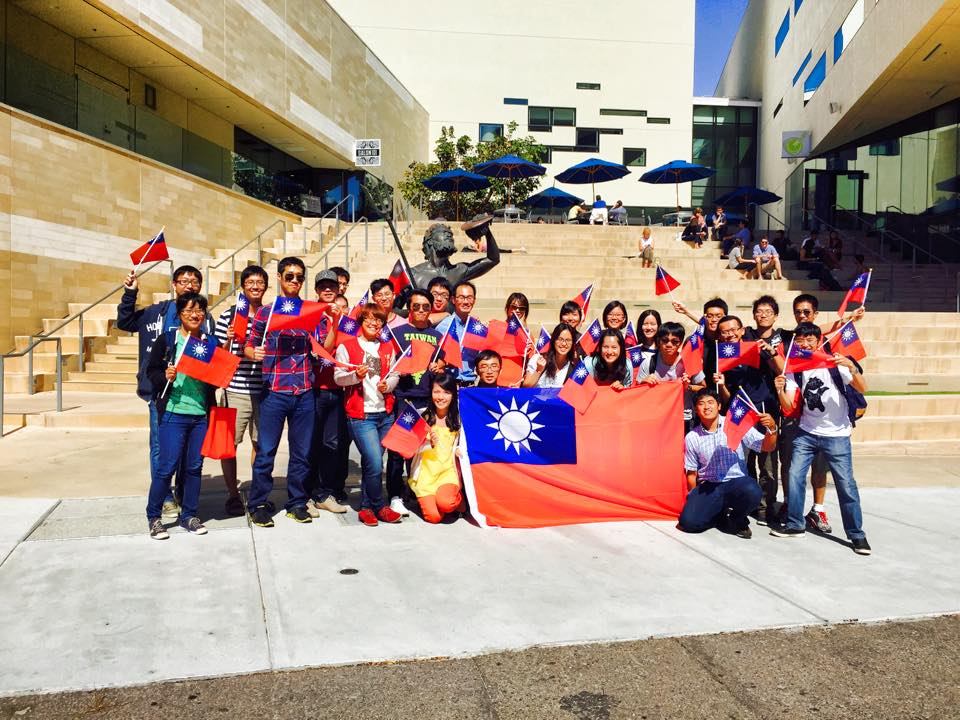
\includegraphics[width=0.43\textwidth]{Pics/pctriton1-min}
\caption{校內飲食以及許多學生活動都集中在 Price Center。(左)Price Center 中午時分的熱鬧樣貌。(右)國慶日時 TGSA 成員們帶國旗聚集在 Price Center 前的海神像地標慶祝。左圖引自\url{http://publications.ucsd.edu/image-library/campus.php}。}
\end{figure}

\item Croutons:在Student Service Center二樓,提供沙拉、三明治、濃湯等餐點。

\item Blue Pepper:一間獨立泰式餐廳,在 Muir College(student center),有些人覺得他的食物比 PC 的亞洲食物還推,吃膩 PC 時可以試試。

\item Dining Hall:共有六間散落在各學院,雖然主要目的是提供給大學部學生用餐,但其實任何人都可以入內享用。平常是以單點供餐,然而在暑假期間部份 dining hall 會改成吃到飽自助餐形式,是大快朵頤的好機會,用 Triton Cash 結帳可以打九折。\footnote{位置參考\url{http://hdh.ucsd.edu/DiningMenus/}。}
\item 其他:每週二PC海神像前廣場會有農夫市集,約十攤左右販賣農產及餐點。除此之外,校園各處還隱藏各式特色餐廳、咖啡車,有空多探索校園會有意外發現。
\end{enumerate}

\section{住宿}
\label{sec:housing}
\subsection{校內住宿簡介}
美國宿舍與台灣的宿舍最不同的地方在於這邊全都是家庭式的,除了臥房外每間宿舍都會有客廳、廚房和浴室。

UCSD 位在 San Diego downtown 北邊的觀光地 La Jolla,地段房價較高,在外租房金額普遍每月 800 元起跳,不過研究生宿舍租金相當物美價廉(跟其他大學比起來也是如此),\textbf{且每位學生都有住 2 年的權利}。

宿舍基本上可以分成五大區,其中 Coast\footnote{Coast 非常難排,等待時間超過一年,不建議新生申請。} 屬於兩層式建築,散落在草皮中,一棟約有 8--10 間房,而 Mesa Nueva, OMS、SGA 及 Rita 屬於大樓式的,有點像飯店的模式,一條走廊左右都是房間。

\begin{center}
\begin{tabular}{c c c c c c c}
\hline
 & Mesa Nueva & Mesa & OMS & Coast & SGA & Rita \\
\hline
地點 & 校外 & 校外 & 校外 & 校外 & 校內 & 校內\\
附傢俱 & 看房型 & 無 & 無 & 無 & 有 & 有\\
車位 & 有 & 有 & 有 & 有 & 無 & 無\\
臥室 & 1 2 3 & 不同房型不同 & 2 & 2 & 4 & 2 \\
價格 & \$750 & \$653(\$567) & \$603 & \$673.5 & \$504 & \$555\\
\hline
\end{tabular}
\end{center}

OMS、Mesa Nueva、Coast皆有到學校的校車,約15--20分鐘一班,可\href{http://www.ucsdbus.com/}{上網}查詢班次。

學校 housing office 網站上有提供\href{http://hdh.ucsd.edu/docs/ucsdcampusmap.pdf}{宿舍與校園的地理位置圖},並且有各宿舍的內部平面配置介紹:\href{https://hdh.ucsd.edu/arch/pages/MesaNueva.html}{Mesa Nueva}、\href{http://hdh.ucsd.edu/arch/mesa.asp}{Mesa}、\href{http://hdh.ucsd.edu/arch/onemiramar.asp}{OMS building 1--4 平面圖} 、\href{http://hdh.ucsd.edu/arch/docs/Coast_SiteMapFloorplans.pdf}{Coast}、\href{http://hdh.ucsd.edu/arch/sga.asp}{SGA}、\href{http://hdh.ucsd.edu/RAR/}{Rita}。


\subsection{各宿舍詳細介紹(圖)}
\begin{enumerate}

\item Mesa Nueva
\begin{itemize}
\item Studio(單人房)、1B1B(單人房)、2B2B(雙人)、3B2B(三人)。
\item 位於校外(東邊),搭校車到學校約15--20分鐘。
\item 地板:地毯。
\item 車位:停車塔。(住戶免費)
\item 衛浴:衛浴分離。
\item 傢俱:Studio應有盡有,其他什麼都沒有。
\item 水、熱水瓦斯:宿舍費已包。
\item 電、網路:網路皆有。Studio包電,其他電費另計。
\item 郵件、包裹:一戶一郵箱(與室友共用),包裹則要到Office領取。
\end{itemize}

Mesa Nueva 是 2017 年新蓋好的宿舍區,一切設備都較新。宿舍群內附有健身房,設備一直有在更新。圖為 \ref{fig:MesaNueva} Mesa Nueva Studio 房型。Mesa Nueva 最麻煩的是所有的鎖都用房卡系統,每人只能有一張,掉了或者沒帶就要找 Office 開,如果 OIfice 沒開就要找警察,警察效率奇慢,等個 20 分鐘都是有可能的。
\\


\begin{figure}
\centering
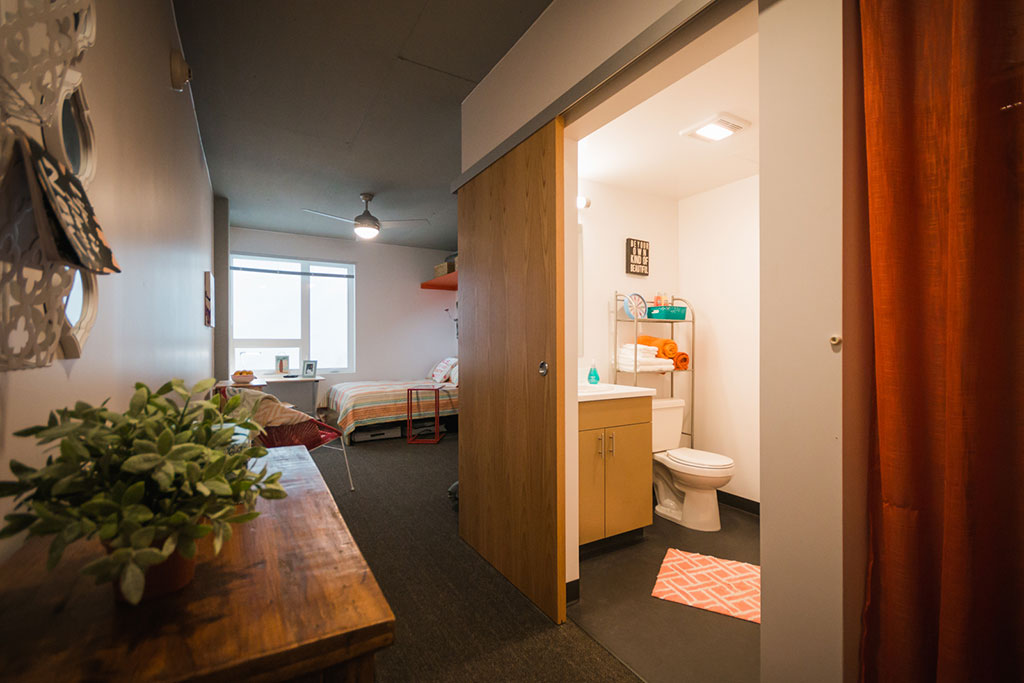
\includegraphics[width=0.9\textwidth]{Pics/MesaNuevaStudio.jpg}
\caption{Mesa Nueva Studio。作為一個人住的房間十分可以接受,唯一的缺點是廚房下面一樣是地毯,手抖一下可能就很難清理。}
\label{fig:MesaNueva}
\end{figure}



\item Mesa(Central, South Mesa Apartments)
\begin{itemize}
\item 兩人一間。
\item 位於校外(東邊),搭校車到學校約15--20分鐘。
\item 地板:地毯。
\item 車位:室外。(住戶免費)
\item 衛浴:衛浴分離。
\item 傢俱:\textbf{無傢俱},廚房僅有冰箱、烤箱和電爐,房間只有衣櫃(後幾頁圖中床、沙發、書桌、燈等皆為自行購置)
\item 水、熱水瓦斯:宿舍費已包。
\item 電、網路:自行牽線付費。
\item 郵件、包裹:一戶一郵箱(與室友共用),包裹則會丟到家門口。
\end{itemize}

Mesa 是小木屋形式的建築,但隔音不好,若有吵雜的室友或鄰居較麻煩,不過是少數。與其他宿舍比起來稍微舊一點,但價格也相對較低。但須要小心最近在進行One Mesa計畫,隨時都有可能把你們趕出去進行都更,風險請自付

\begin{center}
\begin{tabular}{c c}
\hline
Central Mesa & South Mesa\\
\hline
\$567/month & \$652.5/month\\
空間適中 & 空間大 \\
設備較新 & 設備新 \\
\hline
\end{tabular}
\end{center}

Central Mesa 和 South Mesa 皆適合家庭、伴侶。South Mesa 客廳與廚房最大,但房租也最貴,房間與 Central Mesa 差不多大小,二樓有挑高屋頂。圖 \ref{fig:centralmesa} 為 Central Mesa 宿舍內照片。South Mesa 照片請參考 Central Mesa。
\\
\\

\begin{figure}
\centering
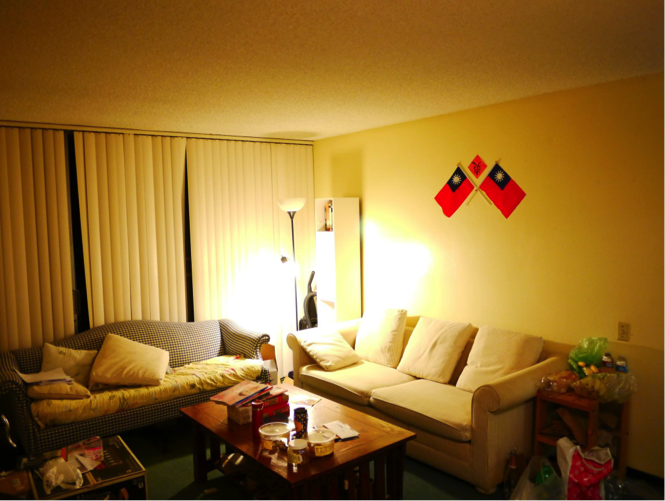
\includegraphics[width=0.45\textwidth]{Pics/central_mesa_1}
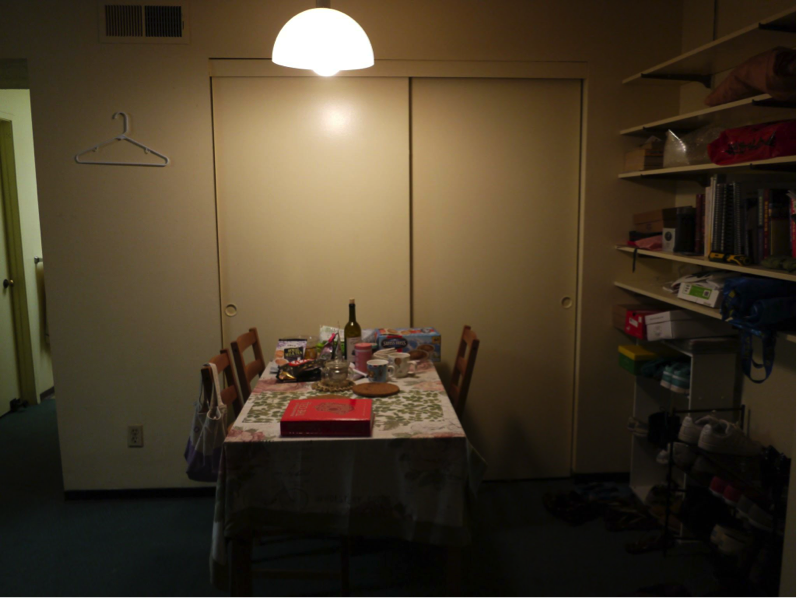
\includegraphics[width=0.45\textwidth]{Pics/central_mesa_2}\\
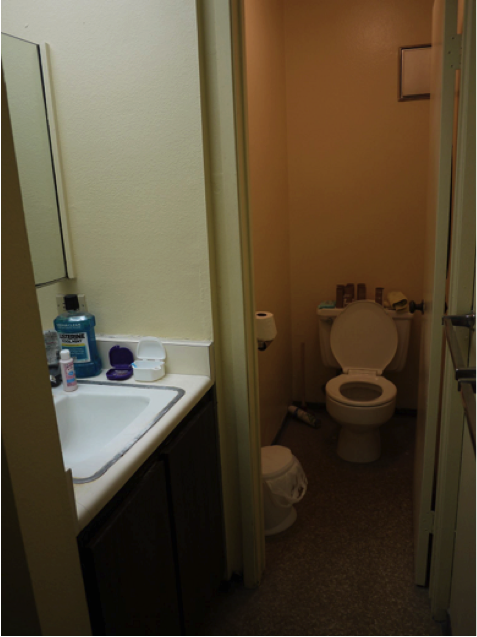
\includegraphics[width=0.3\textwidth]{Pics/central_mesa_5}
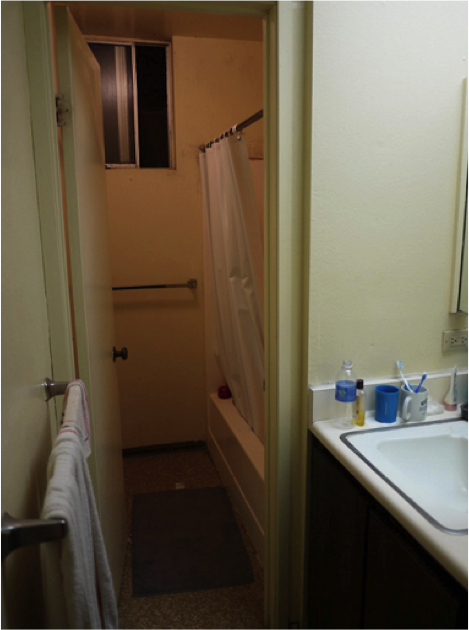
\includegraphics[width=0.3\textwidth]{Pics/central_mesa_6}
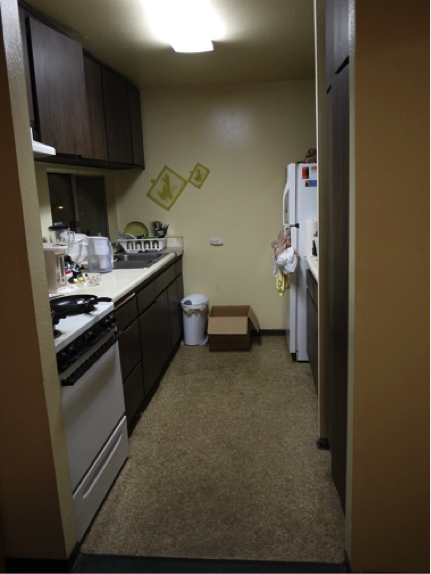
\includegraphics[width=0.3\textwidth]{Pics/central_mesa_7}\\
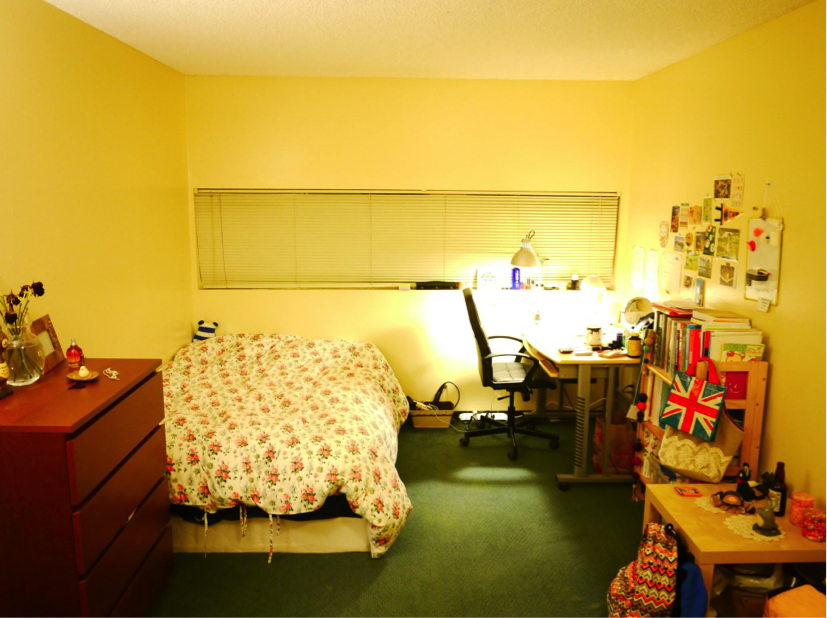
\includegraphics[width=0.45\textwidth]{Pics/central_mesa_3}
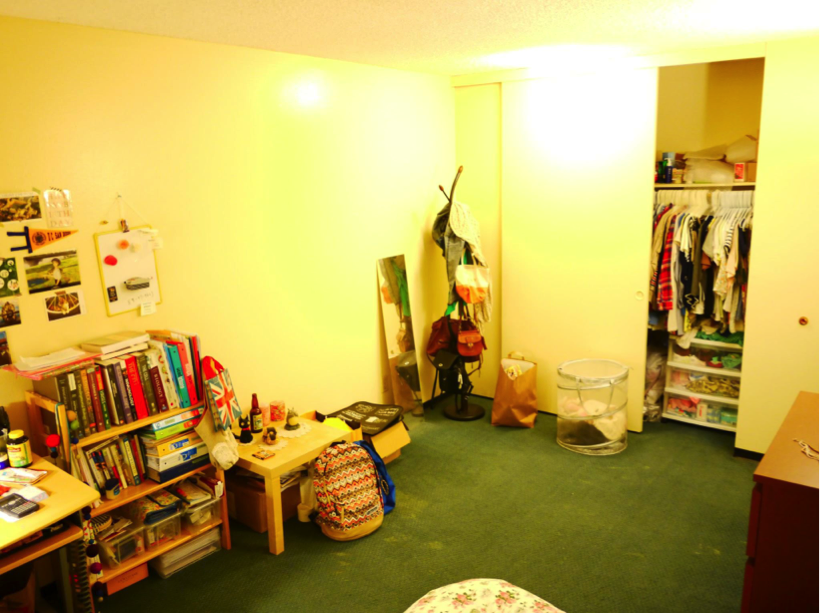
\includegraphics[width=0.45\textwidth]{Pics/central_mesa_4}
\caption{Central Mesa。(左上、右上) 收納空間十分足夠,除了餐桌之外,還可以放得下兩個沙發跟茶几。(左下、右下)房間十分寬敞,有內建式衣櫥。除了 full size 床,其他傢俱擺入房間後仍然十分寬敞。(中左二)衛浴分離,有兩個對稱的洗手台,但是廁所空間稍嫌擁擠一點。(中右一)廚房,流理臺略為擁擠但是可以接受。}\label{fig:centralmesa}
\end{figure}


\item OMS(One Miramar Street Apartments)
\begin{itemize}
\item 兩人一間。
\item 位於校外(東邊,跟mesa在同一區),搭校車到學校約20分鐘;騎腳踏車約15分鐘;走路30分鐘
\item 地板:地毯。
\item 車位:停車塔。(住戶免費。)
\item 衛浴:衛浴分離。
\item 傢俱:\textbf{無傢俱},廚房僅有冰箱、烤箱和電爐,房間只有衣櫃。(後幾頁圖中床、沙發、書桌、燈等皆為自行購置。)
\item 水、熱水瓦斯:宿舍費已包。
\item 電、網路:自行牽線付費。
\item 郵件、包裹:每個人有自己的密碼信箱,包裹則會由 office email 通知再去拿。
\item \textbf{Building 2 外側靠近五號高速公路,24 小時都蠻吵的。}
\end{itemize}
OMS 宿舍內照片請參考圖 \ref{fig:oms}。

\begin{figure}
\centering
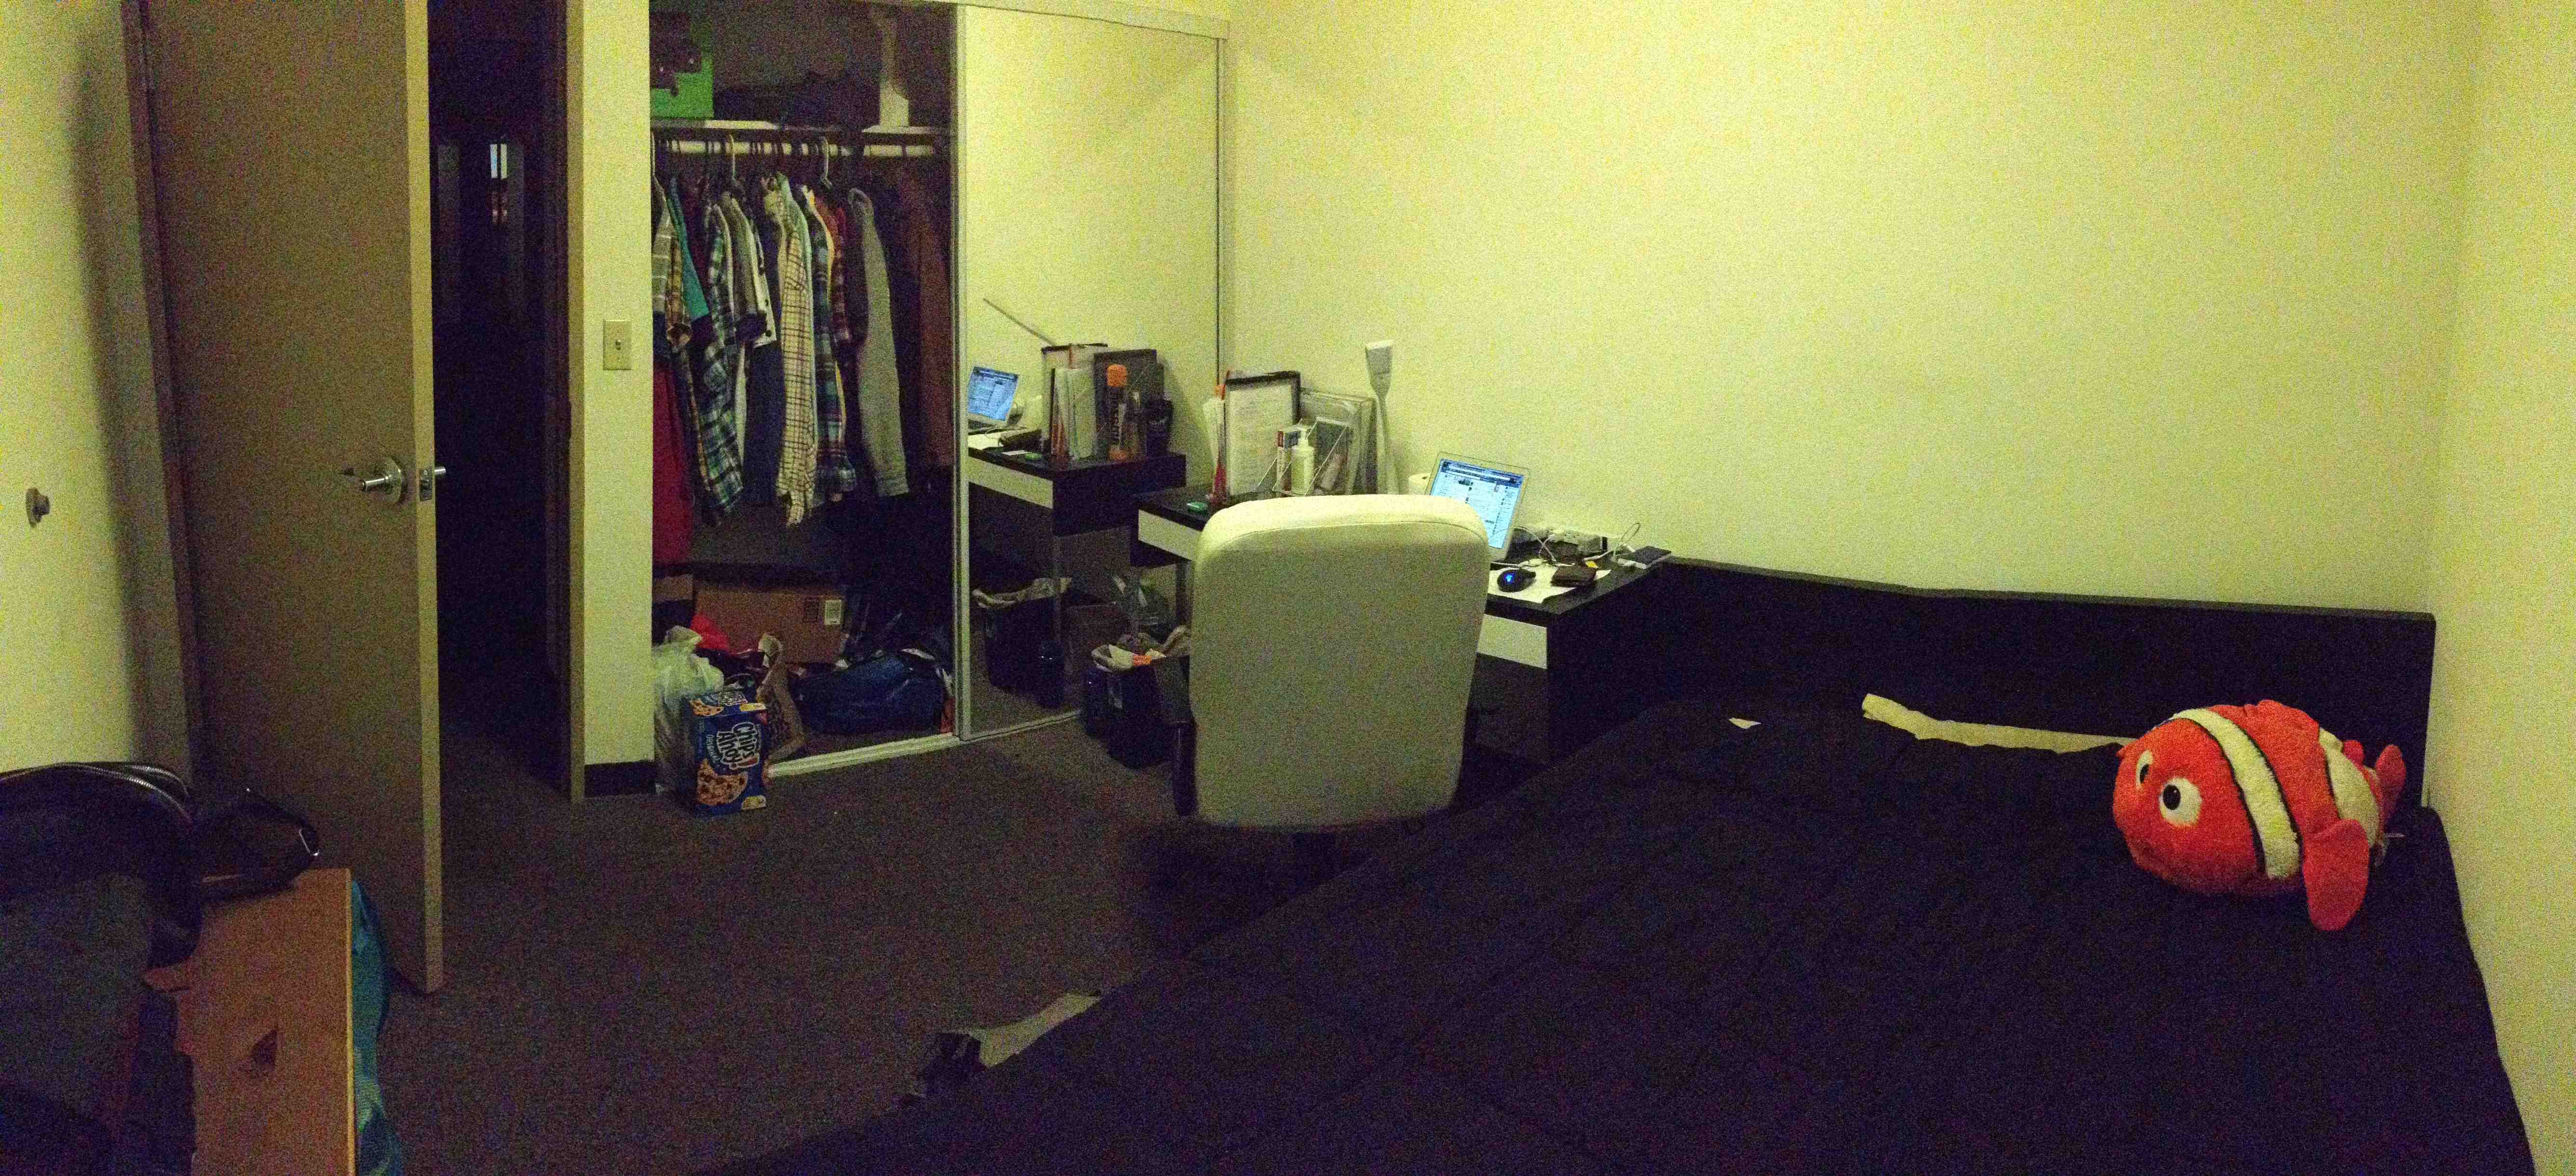
\includegraphics[width=0.67\textwidth]{Pics/OMS_1-min.jpeg}
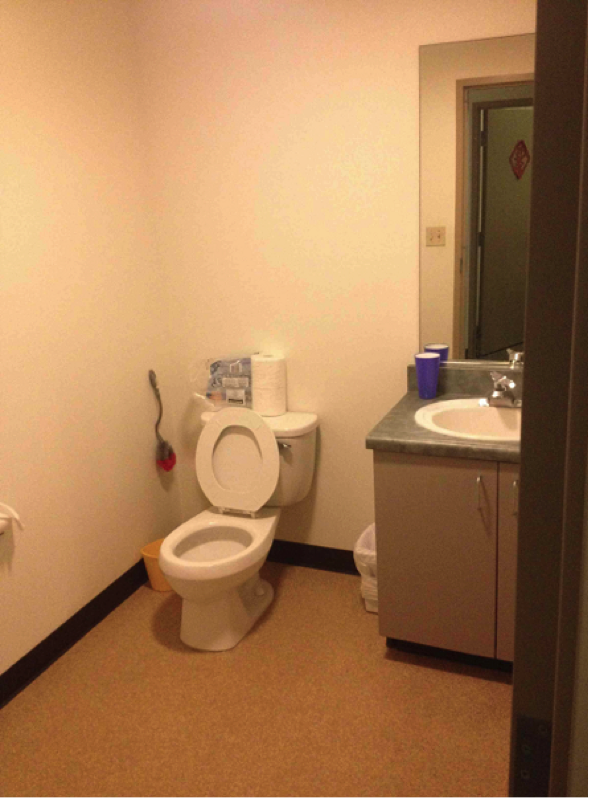
\includegraphics[width=0.23\textwidth]{Pics/OMS_4}\\
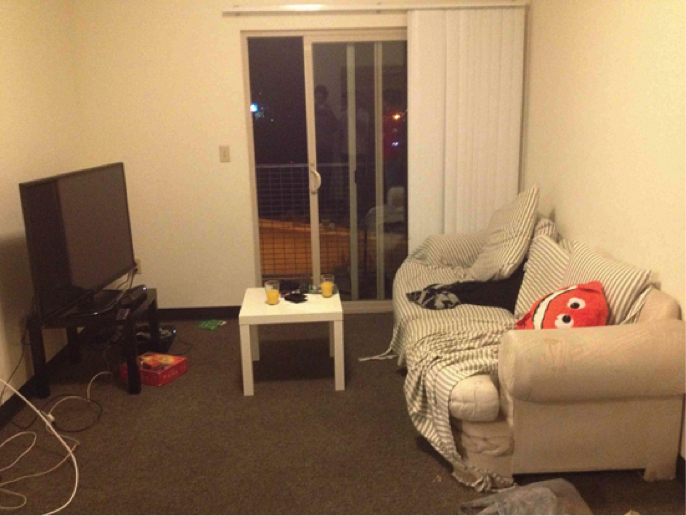
\includegraphics[width=0.315\textwidth]{Pics/OMS_2}
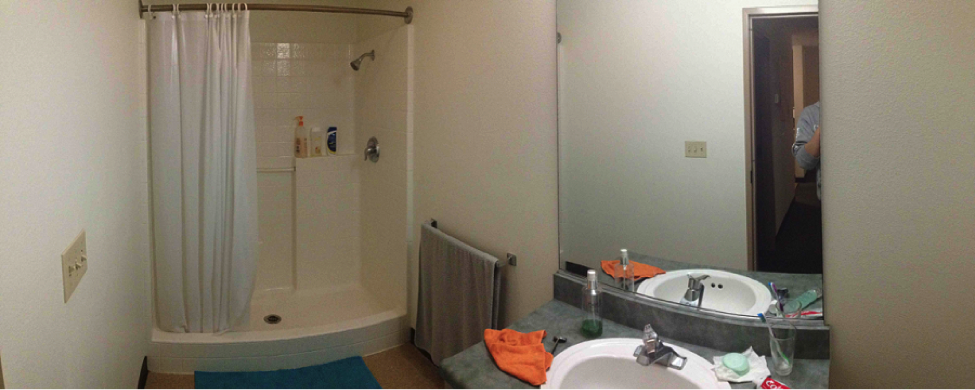
\includegraphics[width=0.585\textwidth]{Pics/OMS_3}
\caption{OMS。(左上)圖中床為 queen size。(右上、右下)衛浴分離,兩間都十分寬敞,浴廁空間是所有宿舍裡算最舒適的。(左下)客廳。}\label{fig:oms}
\end{figure}

\item Rita(Rita Atkinson Residences)
\begin{itemize}
\item 兩人一間。
\item 位於校內,上課或去圖書館都方便。
\item 地板:水泥。
\item 車位:\textbf{無住戶專用車位},若要停車需購置校內停車 permit,約 \$80/month,但車位不易尋找。
\item 衛浴:衛浴合併。
\item 傢俱:附沙發、立燈、書桌椅、床、冰箱,客廳及臥房皆無頂燈,須自行添購燈具照明。
\item 水、熱水瓦斯:宿舍費已包。
\item 電:已牽好,自行付費。(校內優惠價格,十分便宜。)
\item 網路:自行牽線付費。
\item 郵件包裹:每個人有自己信箱,包裹會由 office email 通知再去簽收。
\end{itemize}
Rita 宿舍內照片請參考圖 \ref{fig:rita}。

\begin{figure}
\centering
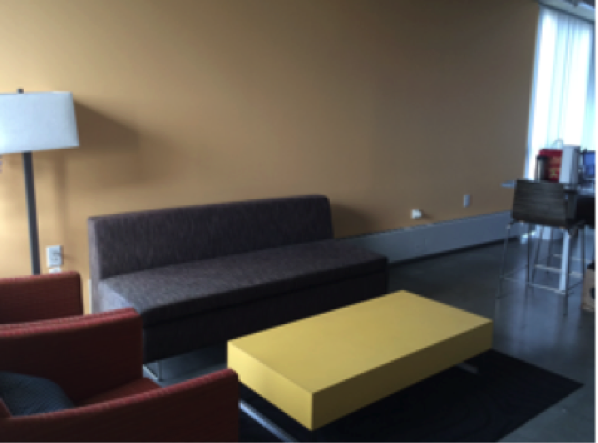
\includegraphics[width=0.455\textwidth]{Pics/rita_1}
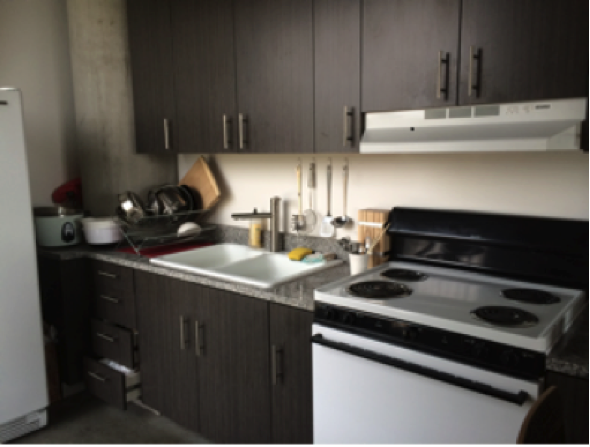
\includegraphics[width=0.445\textwidth]{Pics/rita_2}\\
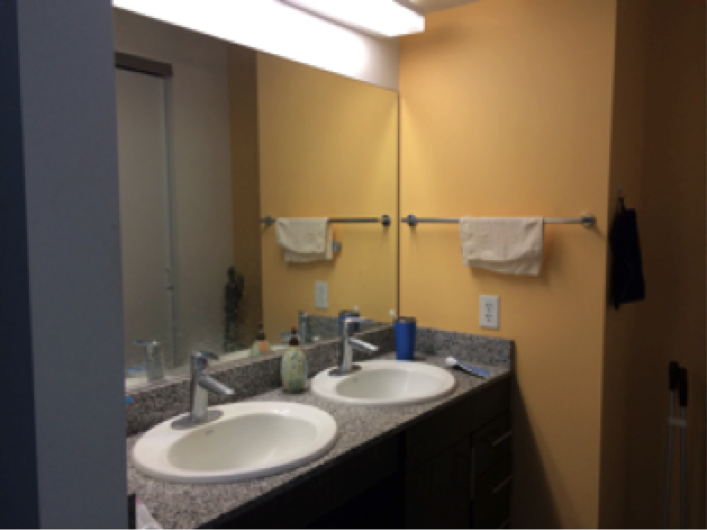
\includegraphics[width=0.45\textwidth]{Pics/rita_3}
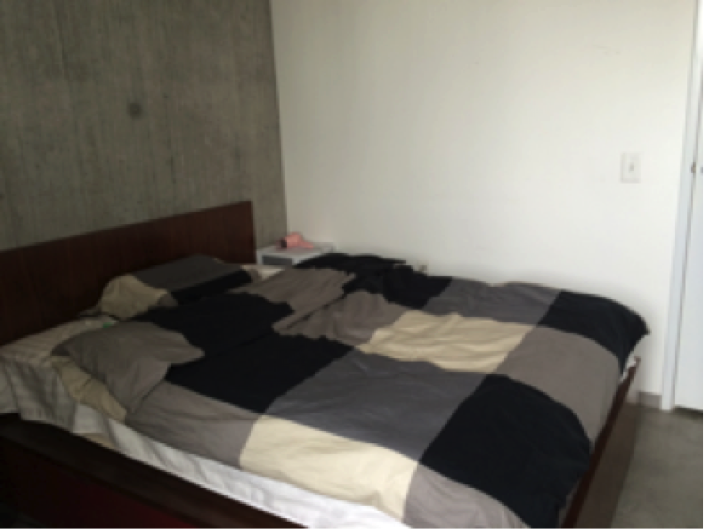
\includegraphics[width=0.45\textwidth]{Pics/rita_4}
\caption{Rita。(左上)客廳,圖中傢俱為學校提供。(右上)廚房大小適中,設備非常新。(左下)單衛浴不過有兩個洗手台,早上不怕搶。(右下)房間大小適中,圖中為 full size 的床。}\label{fig:rita}
\end{figure}

\item SGA(Single Graduate Apartments)
\begin{itemize}
\item 四人一間、人數最多且個人房間最小。
\item 位於校內,上課方便。(靠近工學院。)
\item 地板:地毯。
\item 車位:\textbf{無住戶專用車位},若要停車需購置校內停車permit,約 \$80/month,但車位不易尋找。
\item 衛浴:衛浴分離。
\item 傢俱:沙發、立燈、書桌椅、床 、櫃子、置物架、冰箱。
\item 水、電、網路、熱水瓦斯:宿舍費已包。
\item 每週有人打掃公共區域(廁所、客廳、廚房)。
\item 郵件包裹:每個人有自己信箱,包裹會由 office email 通知再去簽收 \footnote{若非 Fedex 或 UPS 等快遞信件,會送到學校的Mail Services Parcel Center,並寄信通知領取。Fedex 或 UPS 的包裹可直接在 SGA 的 office 領取。}
\end{itemize}
SGA 宿舍內照片請參考圖 \ref{fig:sga}。

\begin{figure}
\centering
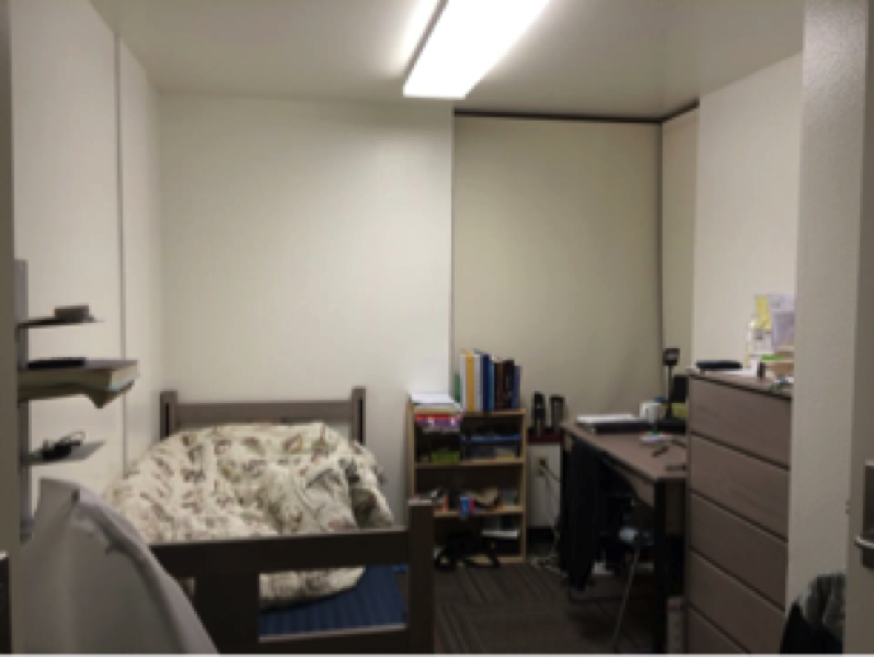
\includegraphics[width=0.43\textwidth]{Pics/sga_1}
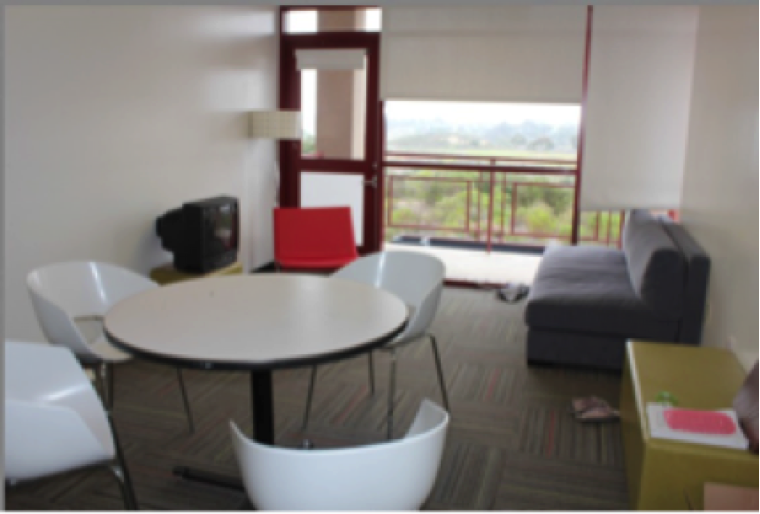
\includegraphics[width=0.47\textwidth]{Pics/sga_2}\\
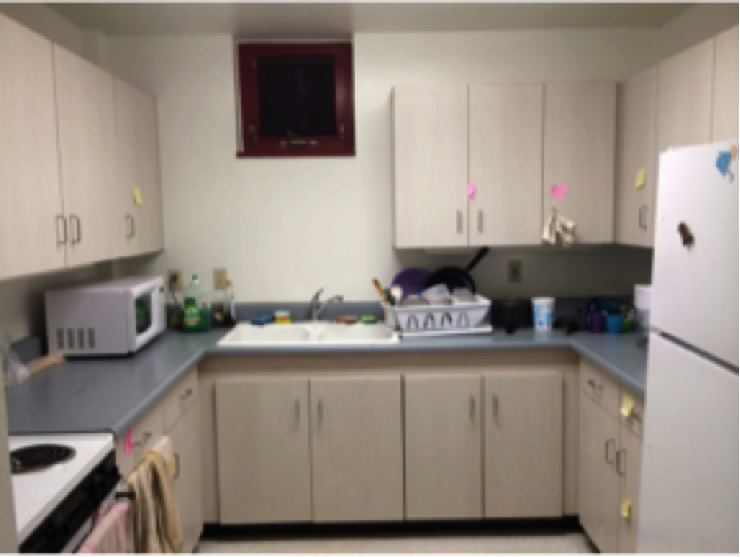
\includegraphics[width=0.35\textwidth]{Pics/sga_3}
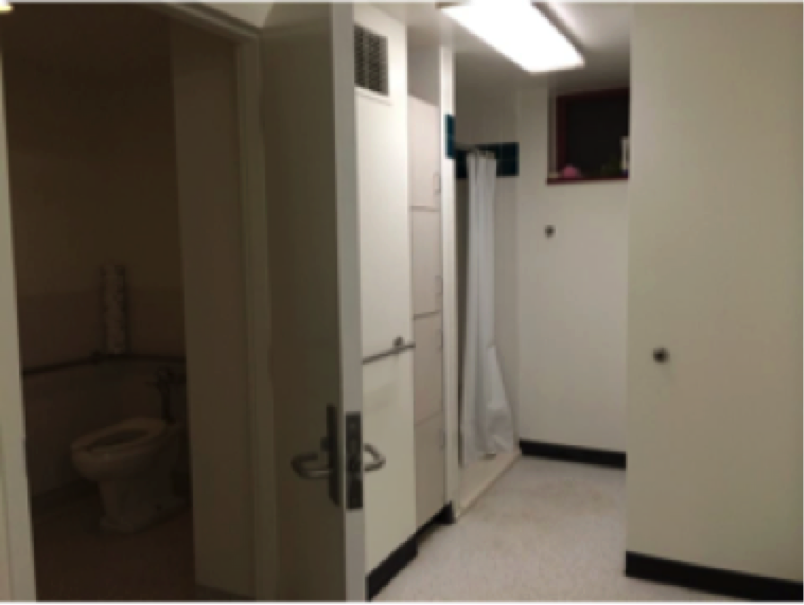
\includegraphics[width=0.35\textwidth]{Pics/sga_4}
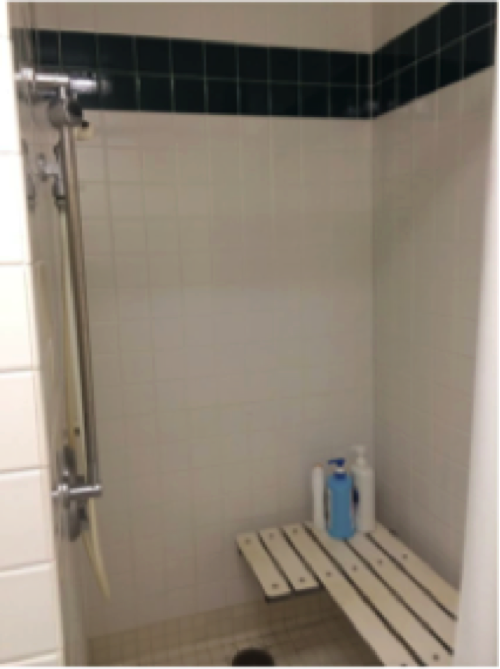
\includegraphics[width=0.2\textwidth]{Pics/sga_5}
\caption{SGA。(左上)房間,床為 twin size,房間大小是所有宿舍裡最小的。(右上)客廳大小中等,圖中桌椅皆為學校提供。(左下)廚房大小適中,但四人共用冰箱,空間略嫌不足。(中下、右下)衛浴分離,有兩個洗手台。}\label{fig:sga}
\end{figure}

\item Coast
\begin{itemize}
\item 兩人一間。
\item 位於校外(西南側),騎腳踏車到學校約8分鐘,走路20分鐘
\item 地板:地毯。
\item 車位:室外(住戶免費)。
\item 衛浴:衛浴合併。
\item 傢俱:\textbf{無傢俱},廚房僅有冰箱、烤箱和電爐,房間只有衣櫃。
\item 水、熱水瓦斯、網路:宿舍費已包。
\item 電:自行牽線付費。
\item 郵件包裹:一戶一郵箱(與室友共用),包裹會丟到家門口。
\end{itemize}
Coast Apartment比其他宿舍稍為難排一點。走路10--15分鐘就能到海邊(Shores),風景優美,衝浪方便。缺點是屋齡較老舊,廁所跟廚房設備都較舊空間也稍小,廚房水槽沒有食物攪拌器,另外若住一樓可能會較潮濕。
Coast 宿舍照片請參考圖 \ref{fig:coast}。

\begin{figure}
\centering
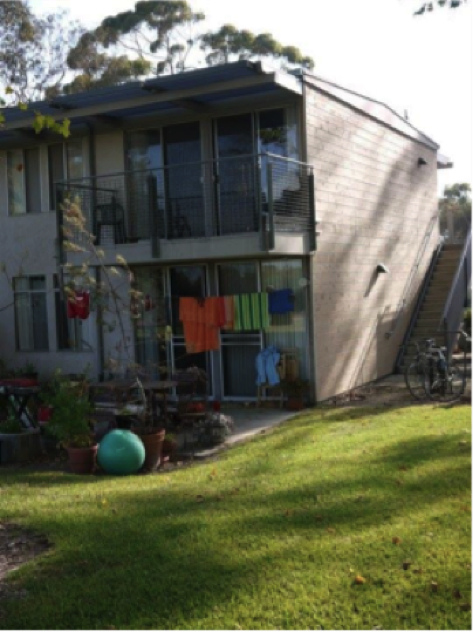
\includegraphics[width=0.3\textwidth]{Pics/coast_1}
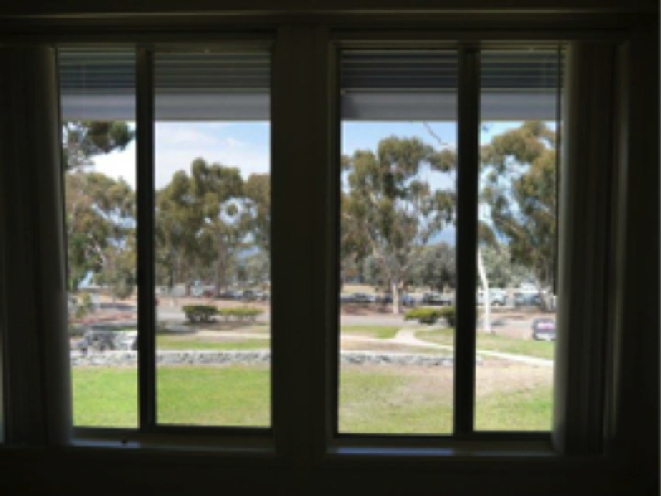
\includegraphics[width=0.6\textwidth]{Pics/coast_2}
\caption{Coast。(左)外觀,房屋建築類似 Mesa。(右)室內窗景。房間及廁所圖請參考 North Mesa。}\label{fig:coast}
\end{figure}

\end{enumerate}

\subsection{宿舍申請}
UCSD 研究生宿舍需透過網路\href{https://hdh.ucsd.edu/ARCHWaitList/ARCHMainMenu.aspx}{線上申請}。線上申請分析:

\begin{enumerate}
\item 申請時間點:越早越好,各位新生們\textbf{一確定要來 UCSD 就一定要先上網申請!!}
\item 申請小技巧:申請時要填入住日期,fall 入學的同學們因為競爭激烈, 建議將入住日期往前填,根據前年經驗,7、8 月太多人競爭,入住日期填在 7 月中以前比較保險。固然繳費就要從入住日開始算,不過比起沒排到宿舍,最後得要住外面,仍然很划算。假如還是沒排到的話,將地段、房型皆改為 any,也會提高排到宿舍的機率。
\item 給 offer 的順位:入住日期(最接近,而不是最早)$>$ 申請日期 $>$ 志願序。

例如,假設今天有個 6/20 的 Rita 2F 房間空出。有將 Rita 2F 列進志願序的(不管第幾志願)的都會依 application date 列出來:

\begin{center}
\begin{tabular}{c c c p{3cm}}
\hline
學生 & 入住日 & 申請日 & 志願序\\
\hline
A & 7/20 & 4/12 & Rita,Mesa,OMS\\
B & 6/09 & 4/13 & Rita,Mesa,OMS\\
C & 6/18 & 4/14 & Mesa,Rita,OMS\\
D & 6/18 & 4/14 & Rita,Mesa,OMS\\
E & 6/18 & 4/15 & Rita,Mesa,OMS\\
\hline
\end{tabular}
\end{center}

這樣的話會由 D 得到住宿權,因為他的入住日期最接近又比 E 早申請,但其實這是由 housing 工作人員主觀判斷,所以基本上越早填,入住時間越早(空房多),排到的機會就越大\footnote{已經提交申請住房表格的同學,可以任意修改表格上的信息,不會影響申請的起始時間。}。

\item 電話詢問:若一路等到七月都還沒有排到宿舍,不妨直接打到 housing,詢問申請狀況,等他幫你確認後,問他可不可以幫你提前入住日期,如同先前講的,排宿舍有時是工作人員主觀判斷,跟他這樣盧一下,很有可能就排到了。

\item 房型選擇:在網頁中可以填三個,依個人需求填入自己的前三志願。

\begin{itemize}
\item 有計劃買車的人:推薦 Mesa Nueva、OMS、Mesa、Coast。(Coast 比起另外三者會稍微難申請上)原因無非就是有附停車位,至於要哪一間就看個人喜好了,在 UCSD 除了搭 Shuttle 去學校以外,去其他地方不開車都很不方便。

\item 想住在校內的人:推薦 Rita、SGA,可走路上學,但若計劃買車則須注意停車位問題。

\item 愛好大自然:首選 Coast、次選 Mesa。(注意:Coast 不好申請上。)Coast 走路 10--15 分鐘就到海邊,最接近大自然,風景優美。Mesa 一走出門即是草皮,但相對的都比較潮濕一點,尤其是 Coast。
\end{itemize}
\end{enumerate}

\subsection{Housing FAQ}

\begin{enumerate}
\item Graduate Housing 能住多久?

不論碩士或博士研究生都只有住兩年的權利。除非得到 SHORE(Student Housing Opportunity Recruitment Enhancement Program)的獎勵,這樣就沒有兩年限制,各位同學在期限到之前就要加緊開始找房子摟。

\item 伴侶或另一半?

只要有一方是 UCSD 的研究生,即可申請 couple 入住,未婚情侶或是已婚夫妻皆可,唯一不一樣的是在申請時要填 couple 入住,並填入另一半的姓名,並在入住時提供以下其中兩項證明:
\begin{itemize}
\item Joint ownership of a motor vehicle.
\item An insurance policy held by one partner that names the other as a beneficiary.
\item A will on behalf of one partner that names the other a beneficiary.
\item Executor or durable power of attorney granted by one partner to the other.
\item Joint responsibility for loans/debts, i.e., credit cards.
\item Joint ownership of property.
\item Joint checking or savings account.
\item A contractual financial arrangement that obligates each of the two parties to provide support, and in the event of termination of the partnership, provides for an equitable division of any joint property.
\item Previous recognition as partners under the policies of another university, company, or municipality, city or state registry.
\item Legal recognition as a family by an outside entity such as a church community.
\item Other documentation may be submitted for consideration.
\end{itemize}
最常見的除了結婚證明外,就是銀行的共同賬戶、汽車保險。\textbf{Couple 仍然只能住兩年,除非有小孩,即可以一路住到畢業。}

\item 沒傢俱怎麼辦?

可以上 TGSA 的 Facebook 社團看有沒有畢業的學長姐要賣傢俱,或是上 UCSD 的\href{https://www.facebook.com/groups/UCSDfreeforsale/}{二手物品平台}看看。建議可以帶個小睡袋過來,以後出去玩也可以用。在開學的前後一兩週,我們 TGSA 也會開幾團帶新生去 Ikea 買傢俱,時間點請再關注 TGSA 的 Facebook(\href{http://www.walmart.com/}{ Walmart }及\href{http://www.amazon.com}{ Amazon }也可以線上購買傢俱)。

\item 電跟網路怎麼牽?

牽電:牽電比較麻煩一些,先上 \href{www.sdge.com}{SDGE 網頁}上預約,在沒有 SSN(social security number)的情況下,除了需要一筆押金,還需要帶著護照跟地址去 downtown 的 SDGE 一趟(要先開好銀行戶頭)再跟著 SDGE 的服務人員指示做就可以了。(他可能會叫你打通電話過去,電話那頭有人跟你確認身份後給你一組數字,再把那組數字給櫃檯。)

牽網路:基本上大部份人都牽 \href{http://www.att.com/}{AT\&T} 或是 \href{http://www.timewarnercable.com/}{Time Warner Cable} 這兩家,根據地址的不同,不一定哪一家比較好。基本上直接上他們網頁預約,就會有專人到你家來幫你安裝,在沒有 SSN 的情況下,也要再一筆押金。建議可自行購置modem及router,則可省下網路公司專人到府安裝費及每月租借費。

\item 寵物?

Graduate housing 都不允許養狗,但有幾處可以養貓,養貓的同學需要付 \$250 押金。

\item 申請上了,學校如何通知我?

若排到房子了,學校將會寄 email 通知房型與房號,若不喜歡,有一次可以拒絕 housing 的機會,再排到時一樣會用 email 通知,若再度放棄將視為此次申請無效,需要重頭來過。\textbf{務必在48小時內回覆 email,否則 housing 將視同你放棄這次機會。}一般在三、四月申請七月底入住的同學不太需要擔心排不到宿舍。

\item 申請上宿舍之後的入住流程?
    \begin{enumerate}
    \item 在 48 小時內回覆 housing 之後,housing會要求先繳 100 元的押金和第一個月房租。
    \item 在入住當天上班時間前往 housing 簽一些文件跟拿鑰匙即可\footnote{若入住日非上班時間,可事先跟 housing 聯絡,他們辦公室外面有密碼箱,會將鑰匙放在裡面並給你密碼,到上班日時再補簽文件即可。}。(申請 couple 房的當天要帶齊兩樣證明。)
    \end{enumerate}
    
\item 如何繳房租?

若人還在台灣,可去銀行開現金支票寄到 housing(不接受信用卡或跨海匯款)。來到學校後可以在 cashier 繳,或是在 \href{http://students.ucsd.edu}{TrironLink} 線上轉帳。繳費日期是設定在每月一日,若是在月中入住,將會用天數計算收費。例如:小湯 6/27 入住宿舍,housing 將會收取(6 月房租 / 30天 $\times$ 4天)的錢。

\item 住不習慣,想換房?

若是覺得房間不好,或是遇到惱人的室友又無法溝通,建議在 1 月時再度提出申請,當時因為淡季,宿舍十分好排,流程就跟第一次申請一樣,並不會影響到 2 年的住宿權利,而費用部分如同月中入住,未滿整月將用天數計算。
\end{enumerate}

\subsection{校外住宿}
沒排到宿舍,人又在台灣,我該怎麼辦?

\begin{enumerate}
\item 首先尋找下飛機後來 SD 暫時居住的地方。
    \begin{enumerate}
    \item 最簡單的方法,住飯店或旅館,但這費用相對較高。
    \item 上 TGSA Facebook 社團尋求協助,通常新生都會提早半個月到一個月來學校,這時許多學長姐仍在台灣或在別處實習,有很大的機會可以找到暫時出租的房間或是客廳。
    \end{enumerate}

\item 尋找校外住宿。

學校附近有許多由管理公司經營的家庭式公寓,房型通常有1B(Bed)1B(Bath) 、2B2B 到 3B2B 不等,平均一個人月租大都在 \$700-\$900,若多人共享一個房間或是住客廳,平均房租可能比研究生宿舍便宜,但是缺點是需配合他人作息及較無隱私。建議找房子之前先找好室友,否則自己一個人要負擔相當昂貴的租金。最好的組隊時機就是新生說明會,屆時可以先尋找同樣沒有排到宿舍的同學,一般來說,說明會都會在七月初舉行,若是這時還沒有排到宿舍,建議趕快開始尋找校外租屋作為備案。\href{https://www.facebook.com/groups/13591139149/}{TGSA Facebook }社團不定期都會有人在徵室友。此外,想認識新面孔也可以上\href{https://offcampushousing.ucsd.edu/}{ UCSD Off-Campus Housing }網站徵室友( UCSD Off-Campus Housing 需要 PID 碼才能申請進入)。

\item UCSD Off-Campus Housing 網站攻略。
    \begin{itemize}
    \item 你可以在上面搜尋 available roommates 或張貼自介文將自己變成 available roommate。
    \item 可以依地段、室友身份(UCSD學生?非學生?皆可?)日期、房型來搜尋房間。
    \item 離學校較近的地段為 La Jolla、UTC、University City。
    \item 在 Off-Campus Housing 網站上找到的全空房大部分為私人出租,對於剛到的新生比較推薦跟管理公司經營的公寓租房子,不管是簽約或是管理上比較有一套標準。
    \item 以下是當時使用此平台租屋的經驗,本來以為會排到宿舍,但等到七月初覺得沒有希望,就開始每天上去看一下空出來的房,在七月底剛好找到 La Regencia 這個社區有個 2B2B 的空出 1B,租屋時間是 9 月初到 11 月底三個月。跟一個朋友一起 share 一個房間(房間頗大),並且繼續排宿舍。當初是透過上面留的 email 跟出租的 UCSD 的學生聯絡,所有文件都線上處理,我們有提供財力證明與 I-20 檔案,加入合約也是在線簽名完成。
    \end{itemize}
    
\item 找房流程。
    \begin{enumerate}
    \item 上各個管理公司經營的房屋出租網頁看平面圖(Floor Plan)、設施(Amenities)及地點。另外,craigslist 是一個很大的租屋網頁平台,但是缺點就是品質難以保證,要多花時間研究。
    \item 網頁上有時候空房更新速度較慢,建議先透過 email 寄信問 leasing office 有沒有空房,或是最早的 move-in date 是什麼時候。若是有朋友在 San Diego 或是自己提早到能夠現場看房的話,建議直接到 leasing office 去現場看房,並跟服務人員拿簽約的資料回家研究,並且詢問簽約時需要準備哪些文件及入住時間;若是無法親自去看屋,只能透過 Yelp 去查一查該社區的評價以及其他人的評論。

    \item 以下是當時租屋的經驗,人在台灣,只透過email和電話聯絡:台灣和聖地牙哥有 15 個小時的時差,所以聖地牙哥這邊 leasing office 普通上班時間都在 8:30a.m.-9:00a.m.,台灣大概是 12:00a.m.-1:00a.m.,先透過 email 確認有空房後,隨即打電話到 leasing office 跟 manager 確認,並且詢問需要準備什麼資料給她。當時我傳了 I-20、VISA、Passport Photo Page 及財力證明。接著 Manager 會要求你填一些基本的線上 application(各公司可能有些許差異):Legal Resident Form、Proof of Income、訂金部分是用 Cashier’s check or Money Order(通常是 \$500 或一個月房租再加上 application fees)、Rental Criteria Form and Initial Rental Agreement and addendums(簽名後掃描再傳回去)。通常管理公司都會要求要幾天內收到訂金的支票,不然無法幫你保留空房,這部分就因每個manager而異。此外校外住宿還要保租借人保險(Renters insurance),不同社區應該有不同合作的保險公司,有很多種方案可以選擇(月/季/半年/一年),之後現場簽約時要帶紙本的 Renters insurance 交給 leasing office。等到訂金部分沒問題後,跟 manager 說好入住日期後,剩下文件就是等到美國後再去填寫。
    \end{enumerate}
    
    以下是幾個學生比較常住的社區,可以參考:
        \begin{itemize}
        \item \href{https://www.gardencommunitiesca.com/communities/costa-verde-village/}{Costa Verde}.
        \item \href{https://www.gardencommunitiesca.com/communities/La-Regencia/}{La Regencia}.
        \item \href{http://www.nobelcourt.com/}{Nobel Court}.
        \item \href{http://www.thepremiereresidential.com/properties/san-diego/la-scala/}{La Scala}.
        \item \href{http://www.regentslajolla.net/}{Regents}.
        \item \href{http://www.avanalajolla.com/}{Avana}.
        \item \href{http://www.torreypinesapts.com/}{Torrey Pines Village}
        \item \href{http://www.axiomlajolla.com/}{Axiom La Jolla}
        \end{itemize}

\item 找房注意事項。
    \begin{enumerate}
    \item \textbf{動作要快!}八、九月有大量新生湧入,你會發現各個公司的空房都不多,是先找好室友,才能快速完成租屋流程。
    \item 附近是否有公車或校車可以到達學校(公車41、201、202、150..等等),UCSD學生證貼上bus sticker可免費搭乘。(\href{http://www.ucsdbus.com/map}{校車路線}、\href{http://transportation.ucsd.edu/alternatives/transit/index.html}{公車路線})
    \item 停車位?有些公寓有三間或兩間房間,但車位可能不夠分配給每個住戶,有計劃買車記得先跟室友溝通好。
    \item 這些出租的公寓,絕大部分跟學校宿舍一樣都是沒有傢俱的喔,看房時所看到有傢俱的是樣品屋,基本上除了冰箱、洗衣機這類的大型電器會附之外,客廳跟房間都是空空的。
    \item 若要在校外租屋可先參考\href{ http://cosb.countyofsb.org/uploadedFiles/Tenant%20Landlord%20guide.pdf 
    }{California Tenants Guide}的相關規定,學校\href{http://sls.ucsd.edu/}{Student Legal Services}亦對已註冊學生提供免費法律諮詢,可多加利用。
    \end{enumerate}
    
\end{enumerate}

\section{購物}\label{sec:shopping}
相關地圖請參考此 \href{https://mapsengine.google.com/map/edit?mid=zQtEEXrWDims.kkyPg0OFPdmM}{Google Map}。

\subsection{傢俱及生活用品}
\begin{itemize}
\item Ikea:東西最齊全,床、桌椅、廚具....應有盡有,基本上就跟台灣的 Ikea 沒有什麼差別,離學校最近的 Ikea 位於 Fenton Park。
\item Walmart:San Diego 的 Walmart 現場床或桌椅這種大型傢俱不多,但可以上網買,不過日常生活用品、廚具、枕頭棉被等都可以在這找到,價格相對 Ikea 便宜些,除了這些 Walmart 也有 3C、汽車用品、零食等。
\item Costco:跟台灣的 Costco 大同小異,在台灣申請的會員卡也可使用。
\item Amazon 線上購物:憑學生證可以申請 Amazon Prime 會員,有許多商品可以免運費。
\item Best Buy:電器、電腦用品專賣店,價格都接近原價,若非急需可以在 Amazon 上先找找看。位於 La Jolla Village Square。
\item Ross:主要販賣便宜衣物、也有少部份的生活用品和住家佈置,如窗簾、吊勾等等。最近店家位於 La Jolla Village Square。
\item Marshall:賣各種衣物、廚具、生活用品、簡易家電,這是家商品很雜的店。最近位於 La Jolla Village Square。
\item Target:主要販賣各類簡易傢俱(塑膠箱、鞋櫃、毯子、棉被)生活用品、廚具、簡易家電等等。在 Clairemont 與 Genesee \& Balboa 都有分店,都是開車才比較容易到達。
\item World Market、Pier 1 Imports:有各種居家佈置、裝飾用品、擺飾。前者更可以找到世界各地有趣的雜貨、零食。在 La Jolla Village Square。
\item UCSD Bookstore:絕大多數生活用品皆可在校內 Bookstore 買到,但價格略微昂貴。
\item 二手物品:
    \begin{itemize}
    \item 上 UCSD Facebook 社團裡面的 Free or For Sale 子社團。
    \item 看 TGSA 裡有沒有學長姐要賣。
    \item 上 \href{http://sandiego.craigslist.org/}{Craigslist 網頁},裡面東西很多但人員較複雜,建議看傢俱的時候要結伴成行。
    \end{itemize}     
\end{itemize}

\subsection{Mall、Outlet}
\begin{enumerate}
\item Malls:

    \begin{itemize}
    \item \href{http://www.westfield.com/utc/}{UTC Westfield}:由幾家百貨公司加上一些小店組成,裡面也有電影院和美食街,地點就在學校附近,有到校內的公車都可以搭去 UTC。
    \item \href{http://www.simon.com/mall/fashion-valley}{Fashion Valley}:要開車約20分鐘抵達,形式和 UTC 大同小異,商家更多一些,有著名的 Cheese Cake Factory,也有AMC電影院。
    \end{itemize}

\item Outlets:

    \begin{itemize}
    \item \href{http://www.premiumoutlets.com/outlets/outlet.asp?id=76}{Las Americas}:開車約40分鐘位在美國與墨西哥的邊境,根據經驗,平時並沒有比一般的 mall 便宜多少,可以當觀光景點,上個廁所也能看到美墨邊境的牆。
    \item \href{http://www.premiumoutlets.com/outlets/outlet.asp?id=66}{Carlsbad Outlet}:開車約30分鐘,聽去過的人分享經驗是男生的東西比較多。但對於初次逛 outlet 的朋友來說,這裡的東西已綽綽有餘。
    \end{itemize}

    基本上厲害的 outlet 都離學校有點距離,平時價格也不會便宜到哪裡去,不過若是有節日像是著名的感恩節黑色星期五,這時的折扣會非常可觀,若是非急迫性的物品可以等到有節日特價時再買。
\end{enumerate}

\section{運動}
\begin{enumerate}
\item 體育館:學校有兩個主要的 gym---RIMAC 和 Main Gym,喜歡重訓的同學記得要先去 RIMAC 學生證過卡之後才能通行無阻,例如在 Canyon View 泳池旁也有一個小健身房,就需要過卡過的學生證才能進入,使用健身房及游泳池都會要求簽waiver。

\begin{figure}
\centering
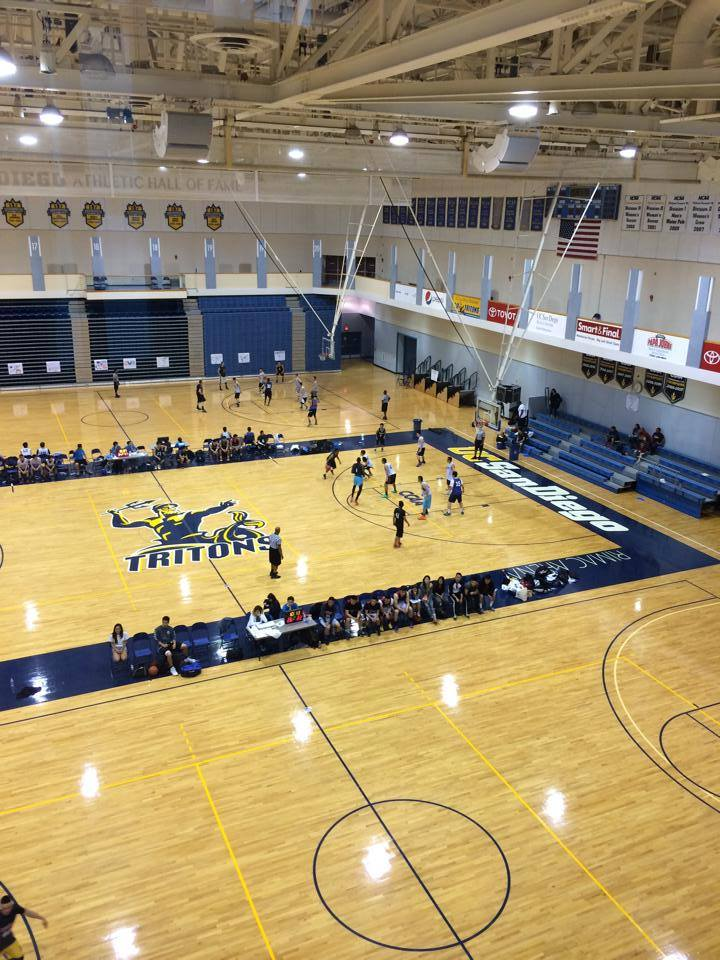
\includegraphics[width=0.32\textwidth]{Pics/rimac}
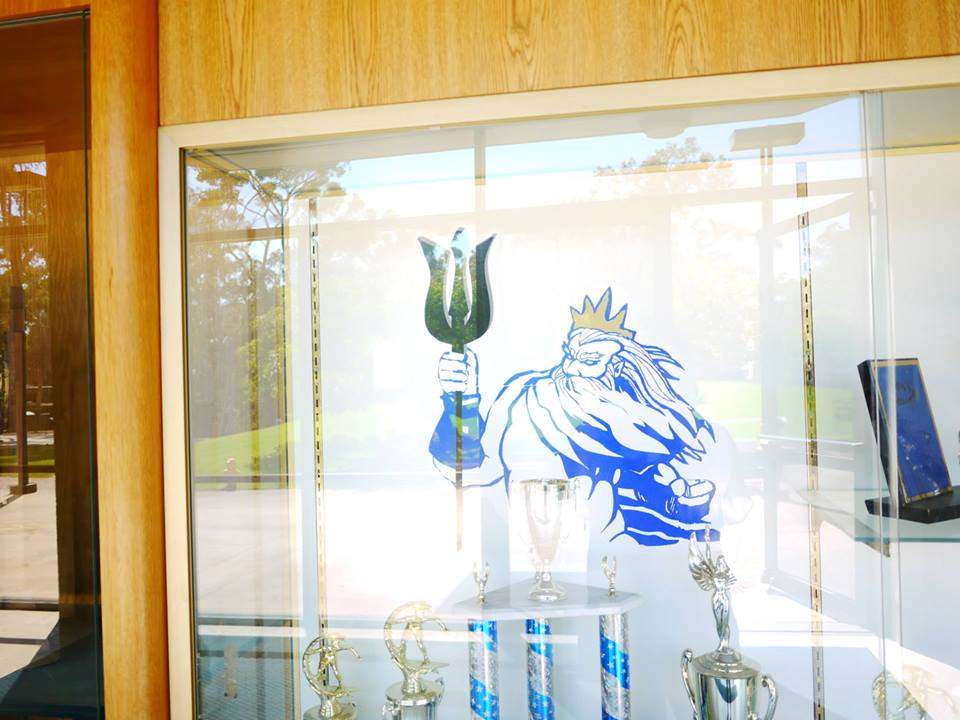
\includegraphics[width=0.58\textwidth]{Pics/maingym}
\caption{UC San Diego 的體育館。(左)RIMAC 體育館內部。(右)Main Gym 主體育館外,櫥窗內的學校精神象徵---海神。}
\end{figure}

Main Gym 及 Rec Gym 都是複合式室內運動場,除了平日白天許多時段為課堂使用,晚上也常常供校隊以及 club 練習,故星期五晚上、週末會是大家主要揪團打球的時間。
學校各種運動的場地非常多(游泳池、籃球、網球、羽球等等),可以參考 \href{http://sportsfac.ucsd.edu/facilities/outdoor/index.html}{網址}。基本上使用這些場地在學期間都是免費的,新生們剛到時還沒開學,部分場地需要收費,且學生保險在開學前是還沒啟用的,要特別注意安全。新生們在自我介紹時,可以說說自己喜歡的運動,TGSA 的 Facebook 社團裡面有許多子社團,學長姐們都會在裡面揪團打球,歡迎大家加入。

\item Recreation class:學校也有提供許多的體育課,例如網球、高爾夫、射箭、擊劍、舞蹈、潛水、體操甚至有如何對抗殭屍的求生課程。這些課程收費一個 quarter 約 \$50 上下。請參考 \href{http://recreation.ucsd.edu/}{UCSD Recreation 網站}。
\item Intramural:即校內競賽,通常為校隊或club主辦,任何在校生都可以組隊報隊,需繳交參賽費依項目上等,有各式各樣多種競賽非常有趣。\footnote{參考\href{http://www.imleagues.com/School/Intramural/Home.aspx?SchID=0b1314dc9a2e48369da7bcd485acebb6}{連結}}
\item 校際競賽:每年洛杉磯經文處會與各校台灣學生合作舉辦多項球類競賽,如國慶盃壘球賽、雙十一盃排球賽、籃球賽等,可以趁此機會參觀各校園、認識他校同學。
\end{enumerate}

\section{英文學習資源}
\begin{enumerate}
\item UCSD Extension %(邵駿澤分享)

在每個學期初,Graduate Student Office 會提供 75 個 voucher,可以換 UCSD extension 400 元以下的課程,如果有拿到的話,在extension 內有一些英文課程,像是 Effective Oral Presentation,可以免費上課。Extension 的上課時間都是晚上,基本上不會跟正課衝堂,所以有時間的話,extension 內的課程是滿不錯的英文資源。

\item I-Center %(徐聖修分享,黃敬心補充)

I-Center 有 \href{http://ispo.ucsd.edu/programs-events/eia/tutee-application.html}{English-In-Action} (EIA)的 program免費提供給國際學生。上網填寫自己的資料、興趣、自我介紹,到I-Center做簡短面試(確認英文程度),然後 I-Center 會幫你配對一個 native speaker。有的是學生、有的是退休的英文老師,重點是這些人都十分熱情。這提供一個平台讓你認識一個興趣相近的好朋友,同時練英文,是很棒的機會。

I-center 也常辦各式各樣的活動,例如週五 international lunch、coffee 等,可以跟其他國際學生用英文交流。感恩節前夕也會有跟 local family 一起享用火雞大餐的活動,這些不只學習英文,也體驗文化。
\end{enumerate}

到美國英文不一定會自動變強,但是英文學習資源非常多(每個人都是你練習的對象),如果有實驗室、修課夥伴,這樣練英文是最快的。

\section{獎學金與補助(TA/RA機會)}

\subsection{獎學金種類與簡介}
獎學金與補助大致分為三種:fellowship(scholarship)、RA-ship(研究助理)、TA-ship(教學助理)。三者補助的方式與金額不盡相同,簡單說明如下。

Fellowship 通常只給 PhD,由系上補助第一年的學費(tuition)和生活費(stipend),目的是給PhD學生專心修課和 lab rotation。第二年之後,就要找指導教授,由他提供你到畢業前的獎學金。

RA-ship 由指導教授從研究計劃裡提供,補助金額與 fellowship 大致相同。基本概念就是他出錢請你做事,因此為了投資報酬率,老板的 RA-ship 通常只給 PhD。不過有少部分的教授會願意提供 RA-ship 給 MS 學生,還是值得打聽與嘗試。

TA-ship 是由協助教授教課來換取補助,又依照每周工作時數分為 25\%(十小時)和 50\%(二十小時)兩種。拿到 TA 之後,除了每個月可以領stipend(50\% 拿的跟fellowship 和 RA 差不多;25\%只有拿一半),學費也可以減免。注意,國際學生拿 TA-ship 還是得付「非加州人」的學費(約五千美金),畢竟UCSD是公立學校。

TA 再細分下去還有一種職位稱為 reader,這份工作只幫忙改作業,不用帶討論課。可以拿到 25\% TA-ship 的薪水,學費也可以減免。

\subsection{申請補助經驗談}
相信你會仔細讀這個 section,代表你急迫的想找獎學金或補助,根據我們的經驗,整理了幾個比較常見的管道和申請技巧。

\begin{enumerate}
\item 找指導教授做研究,勇於爭取:找教授時可以探聽是否會提供 RA-ship 給 MS 學生。勇於找老闆談,歐美的老板對於錢的事情很直接,不如亞洲文化般忌諱。即使老板沒有計劃的錢,也可以問他可不可以當他教課的 TA 或 reader,大部分的老板還是會願意幫自己的學生。

\item 比較有機會申請到的TA:國際學生的優勢莫過於語言教學,以及理工科的基礎科學。在UCSD有中文TA就是值得嘗試,可以在暑假期間留意學校的信箱,會有相關徵人公告寄到信。除此之外還可以詢問化學系或物理系的系上是否有基礎科學的實驗課可以當TA。理工科的同學可以多加申請,並獲得的機會也比較大。

\item 填完申請表,還沒結束!教授通常都會找自己認識或熟悉的學生當助教,因此申請表送出後,可以寫信給教授毛遂自薦,甚至直接去找教授聊聊;或是修過他的課,表現突出讓他印象深刻,都可能成為你拿到 TA 的關鍵。因此如果想要申請TA的人除了寄信給教授外,更應該直接與老師約時間跟老師當面談!越積極的尋找老師是獲得TA的不二法門。

\item Fellowship:美國常見的 NIH 或 NSF 給的 fellowship,國際學生都不能申請。但如果你的研究成果豐碩,或是老闆很給力,也可以嘗試一些給國際學生的 fellowship。亦或是台灣教育部提供給已在國外念 PhD 的乙類獎學金。針對台灣的獎學金,主要分成公費留考、留學獎學金以及尖端科技獎學金。公費留考是台灣教育部提供最豐厚的獎學金,包含了學費和生活費的補助,每年八月會開放報名。而留學獎學金則是針對已經錄取的博士生在生活費上上的補助。每類型的獎學金每年都會有不同的規定與要求,需要申請台灣獎學金補助的學生可以多加留意。當你有自己的獎學金,也意味著老闆在你身上的花費就不需要這麼高,這時候你在研究上的主導性較高,並且研究室的選擇性會較有彈性。 
\end{enumerate}

\subsection{中文 TA 經驗分享}
(MAE MS 胡凱婷)

如果自認為發音標準,簡繁體板書能力普通,有辦法撥出一周三天各一小時的教學時間,有能力用英文教中文(就像以前外國人在台灣交幼幼班英文一樣)就很適合報名。

中文 TA 申請方式原則上就是每個 quarter 開始的前一個月 follow 中文系寄來的申請方法申請就可以了。我當初申請除了完成基本網路填表跟上傳 CV,還有加上錄音跟手寫自介。手寫自介請著重在自己為什麼有能力當中文 TA,錄音的部分我是把自己的經驗再深化描述。

有關手寫自傳,我自己本身在高中是人文相關的特殊班,然後也有幾次的教學經驗跟文字工作經驗,所以我把重點放在這邊,當然如果版面還有空間也可以寫一些看起來很炫的經驗,像是接待外賓之類的。錄音的話,整段時間我都在解釋自己的教學經驗跟從中體會到什麼。在我錄取之後,面試我的老師就有說他們是特別喜歡我的錄音裡所敘述的教學經驗分享,所以錄音部分請未來的申請人也不要太大意。

中文 TA 雖然每次釋出十幾個名額,但原則上都會繼續錄用之前已經是中文 TA 的同學。講白話點,就是當你被錄取成中文 TA 後,你在 UCSD 的就學期間可以一直當中文 TA。但不能因為覺得自己是永久 TA 就鬆懈,我第二季 quarter 時就遇到裁員風波。我的建議是當上 TA 後口音跟英文表達能力要自我補強,然後攏絡學生的心,這樣被裁掉的可能性就會大大降低。

中文 TA 的優點就是不用花太多時間備課,雖然要重新學中國使用的拼音,但在熟悉後中文教學反而是研究生生涯的一段放鬆時間。而且中文 TA 也有意想不到的累積人脈的機會,像我就很幸運認識到 bio 公司相關的人。希望我的小小經驗會幫助到對中文TA有興趣的人。

\subsection{CSE TA 經驗分享}
(CSE MS 蘇仲岐)

每個系甄選 TA 的方式都不相同,以下為 CSE 的情況。

在每個學期結束前(約第 6--7 週),系上會給學生填 TA 申請表,並填上志願序。之後系上會統整名單,交給開課教授選志願(約第 8 週)。志願再交回給系辦,並做出最後決定(約第 9--10 週)。如果有特別想當TA的課,建議在第 6--7 週時先去找教授,可以寫信或直接敲門詢問,這樣當上TA的機會會較高;或是可以得知教授已經決定把 TA 留給他的學生,這樣志願就不用浪費在這門課了。系上甄選的優先順序為 PhD $\rightarrow$ 2nd year master $\rightarrow$ 1st year master,並且會看相關課程成績,以及英文能力(英文是否為母語,及托福口說分數)。以我的經驗看來,英文為母語的學生機會稍大一些。值得注意的是,系上可能會有潛規則來篩選,像是 CSE 要求托福口說要 23 分以上,不然得要利用學校兩種以上增進英文能力的資源(例如在 extension 修過 ESL 課程,international center 的 English-In-Action,Toast master 等等)才有資格被選為TA。

選上TA後,在第一次當 TA 前還要通過 10--20 分鐘的語言測試,包含回答問題和試教,通過才能當 TA。另外,有些系所如 CSE,要求當 TA 前(或同個quarter)必須修過特定課程,如 CSE599 (Teaching Methods in Computer Science)才能當TA。

TA 工作內容包括主持 discussion session,office hour,以及改作業、考卷,輸入成績等等。

薪水和學費減免部分,如果是 25\%(10 hours/week),月薪約為 \$980,50\%(20 hours/week)月薪約為 \$1960。每年、每個系都會有所調整。此外,tuition fee 和保險減為 200 元左右,但還是需要繳 non-resident fee。

\subsection{ChemE Reader、TA 經驗分享}
 (ChemE PhD 陳品瑋)
 
申請方面因為我是 chemical enigneering 的,系辦只要系上開始徵選 TA 或 reader,他們都會把資訊馬上寄信給系上的同學,只要照個網站上的要求與步驟並上傳 CV,然後就是等待結果了。

以我們系而言,通常系上教授都會先挑自己實驗室或者自己系的學生,所以外系要申請到好像會比較困難,但都可以試試看,或者也可以先連絡開課教授問問看他是否還有職位的空缺,反正簡單來說就是有申請有機會。

我剛好在 14 winter 和 14 spring 分別申請到 Reader 和 TA,工作內容其實就是看教授,我在當 reader 的時候就是負責改考卷(25\% 的Reader, 10 hours/week)也不用幫學生解答問題,只要改改考卷改改作業,每兩個星期就會有大約 \$250 (reader 是每兩個星期發一次薪水)再加上我們系的 reader 也可以有學費減免,所以真的還算蠻好賺的。

然後在 14 Spring 的時候我申請到了系上的 TA,開課教授也是人非常好,作業考卷都自己出,解答我也不用寫,也是幫忙改改考卷,比較不一樣的就是要開 office hour 幫學生解答問題,TA 是每個月發一次薪水,我是 25\% 的 TA(10 hours/week)每個月大約可以領 \$980,總而言之其實 reader 或 TA 的工作量還是要看開課的教授。

有關學費減免的部分,每個系好像都有自己的規定,所以在申請前最好都要問過各系的系辦,以免申請到結果學費沒有減免最後空歡喜一場。

\section{F1、J1 簽證問題}
\label{sec:visa}
國際學生在美國念書的身分證明文件,就是 F1 或是 J1 簽證。簽證、護照是在美國出入關及辦事的必備文件,建議多準備影本和掃描電子檔。

收到UCSD錄取之後,下載財力證明,傳真或郵寄給學校,在四月底五月初就會收到學校寄來的 I-20(申請F1) 或是 DS-2019(申請J1)。有這些文件才能到美國在台辦事處(AIT)辦理 F1 或 J1 簽證。

辦理簽證主要資料:
\begin{enumerate}
\item 準備好 I-20 或是 DS-2019 ,以及針對美簽用的大頭照電子檔
\item 至美國在台辦事處的網站上進行填寫相關資料、並進行繳費與預約(\url{http://www.ustraveldocs.com/tw_zh/index.html?firstTime=No})
\end{enumerate}

主要流程:
\begin{enumerate}
\item 填寫 DS-160 表格。所有資訊必須正確且真實無誤。
\item 一旦確定正確的簽證類別並填妥DS-160後,必須支付簽證費用5120台幣(會因匯率不同而有差異)。至郵局或銀行進行繳費,並且必須保留收據號碼,才能安排簽證預約。
\item 重新登入簽證線上系統,並按左側選單中的「安排預約」,隨即開始安排預約的程序。將需要:
\begin{itemize}
\item 護照號碼。
\item 簽證費收據號碼。
\item 顯示在 DS-160 確認頁的 10 位字元電腦條碼。
\end{itemize}
\item 請在預定的日期和時間,前往美國在台協會辦理簽證面談。請務必查看「安排我的預約」頁面,了解面談的必要文件。
\item 護照會被扣留審查,當簽證獲准,簽證(護照)會寄到你所填寫的指定地點。
\end{enumerate}

補充說明:
除了申請美簽以外,還需要完成 SEVIS 系統,並繳交 SEVIS I-901 費用。

SEVIS 記錄:學校會將 I-20 或 DS-2019 的資料輸入到 SEVIS (學生及交換訪客登錄系統)裏。該系統主要是追蹤所有學生及交換學者。
SEVIS I-901 費:所有申請 F-1 、 J-1 簽證的人都必須繳交 SEVIS I-901 費用給國土安全部。

簽證注意事項:
\begin{enumerate}
\item 注意簽證開始日。I-20 或 DS-2019 上會寫最晚入境的日期,通常是學校的 orientation day。特別注意,該日期前 30 天內才能入境。若要用旅行簽証先來美國,則必須於 orientation day 前出境再以 F1 或 J1 身分入境,否則簽証轉換手續既費時又花錢。

\item 注意簽證到期日。不同學位、不同科系,發的 I-20 或 DS-2019 的期限不同。尤其是 J1 簽證要注意,例如公費通常最多補助三年,DS-2019 的期限也只有三年,因此時間快到時必須要向學校申請新的 DS-2019,並回台灣重新辦美國簽證。

\item 旅遊簽章。不論 I-20 還是 DS-2019,表格上有 travel validation by responsible officer 欄位。此欄位必須要 I-Center 的簽名(需花一周),才能離開美國後再度入關。要到回台灣或到別國旅遊前,務必記得。另外,簽名效期只有一年。過了之後必須重新到 I-Center 簽名。若欄位已滿,也必須向學校重新申請 I-20 或 DS-2019。
\end{enumerate}

F1 與 J1 簽證的差異:大部分來美國念書的學生,都是持 F1(學生)簽證。而交換學生、訪問學者、博士後研究員、公費生等拿的就是J1(交換訪客)簽證。J1 的規定較為複雜,有的 J1 簽證(如訪問學者)規定須回台灣居住兩年(Two-year home-country physical presence requirement,會寫在 DS-2019 上),才能在美國工作或申請綠卡。又如公費生的 J1 簽證則有契約書另外詳定。

另一個顯著的差異,若是眷屬申請 F2 或 J2 簽證出國,前者不能工作,後者可以。I-Center 於開學時會辦許多說明會,尤其針對 J1 簽證的規定,若有疑問可以參加詢問。

\section{報稅}
以下的說明主要針對為非居民外國人(non-resident alien),也就是 (1)持F/J簽證 (2)待在美國不超過五年 (3)沒有美國居民身分的留學生

為什麼我每個月的部分收入都已經被提列為稅款了,我卻還要報稅?
\begin{enumerate}
\item 報稅是所有人的義務
\item 由於你實際應繳稅款與薪資扣除額有差異,因此透過報稅的手續可以獲得若干的退稅
\end{enumerate}

沒有收入的人有沒有需要報稅?
理論上要。

一般常見的收入種類與相對應的兩種收入表格(W2/1042-S),美國的報稅制度與台灣相比較落後,還停留在使用紙本的階段。因此在報稅季節(4/15)前學校會透過郵件系統將你上年度的收入明細寄給你,若是你到三月中還沒有收到,很有可能是你在入學的時候沒有填好你的地址資訊,請找各系辦洽詢。
\begin{itemize}
\item W2-所有工資型式的收入(TA、RA),這種收入須要繳聯邦稅(federal tax)及州稅(state tax)。
\item 1042-S-獎學金性質的收入(scholarship、fellowship),這種收入須要繳聯邦稅(federal tax)。
\end{itemize}

以下是新生不會用到,但以後會用到的表格:
\begin{itemize}
\item 1099INT-利息收入。非居民外國人的利息收入是免繳稅的;如果你收到 1099INT,可以用 Form 1040NR 報稅,並在 1040NR 的第五頁 other information 的 question L 中列出利息收入。
\item 1099DIV-投資的利息收入。這部分的收入即使是 non-resident alien 還是需要繳稅的。
\item 1099G-去年州稅退稅金額。
\item 1099MISC-工作以外的雜項收入。
\end{itemize}
UC系統查詢收入明細請見\url{https://atyourserviceonline.ucop.edu/ayso}

聯邦稅:聯邦稅的繳交表格為 1040NR/1040NR-EZ,很幸運的是學校目前使用一個 glacier 的系統來協助你完成報稅。請在開學時就向各系辦洽詢有關 glacier 的註冊。透過 glacier 進入 glacier tax prep 一步一步依照指示填好(在填寫的過程中你會需要用到你的新舊護照以及收入表格(W2/1042-S))。最後系統會要求你印出 1042-S/W2、1040NR-EZ、8843、Grant Statement(印出來要簽名)寄到
\textbf{Department of the Treasury
Internal Revenue Service Center
Austin, TX 73301-0215
USA}

州稅:州稅的繳交表格為CA540NR-short。在州稅的部分,由於UCSD沒有提供像glacier這樣的系統,因此我們就必須要人工填寫,由於填寫的過程中需要用到聯邦稅表格1040NR/1040NR-EZ的資訊,因此請先完成聯邦稅之後再申報州稅,由於表格每年都略有變動,因此我們沒有辦法逐項說明,不過由於每項的結果常常會影響後面的項目,所以請帶著一顆清醒的頭腦細心的填寫。
表格:\url{https://www.ftb.ca.gov/forms/2014/14_540nrshort.pdf}
填寫說明:\url{https://www.ftb.ca.gov/forms/2014/14_540nrshortins.pdf}

經過一段認列扣除額的過程後,你會得到一個數字即為你的taxable income,用這個數字到稅率計算網站https://webapp.ftb.ca.gov/taxcalc/calculator.aspx就可以算出你應繳的州稅。

列印簽名後連著你的 W2、1099(optional)
如果要補稅寄到:FRANCHISE TAX BOARD PO BOX 942867 SACRAMENTO CA 94267-0001
如果要退稅寄到:FRANCHISE TAX BOARD PO BOX 942840 SACRAMENTO CA 94240-0001 

沒有在美國領取任何收入的同學,你要作的是填寫\href{http://www.irs.gov/pub/irs-pdf/f8843.pdf}{8843表格},這個目的是在美國的稅務系統中建立你的身分記錄(只要填寫表頭、part 1、part 3), 簽名後寄到
\textbf{Department of the Treasury
Internal Revenue Service Center
Austin, TX 73301-0215
USA}

\section{就醫}

學校保險的部分,就是照學校合作的保險方案(UC SHIP---Student Health Insurance Plan)一個學季約 \$1138 (詳見學校網頁或是學費明細)。

從 2015 年開始學校不會再主動寄發保險卡,學生可以自行用手機下載 Student Health Mobile App (支援 iOS 和 Android),然後用和學校系統相同的姓名、PID 和生日註冊,註冊後就可以看到電子版本的保險卡。有需要的話也可以打電話到 Anthem 866-940-8306 and/or Delta 800-765-6003 索取實體保險卡,索取實體保險卡會需要保險 ID,如果從手機 App 無法讀取,可以打電話到 858-534-2124 詢問。

若不想使用學校的保險,也可以購買其他符合規定的保險取消UC SHIP。詳細規定請見:\url{https://wellness.ucsd.edu/studenthealth/Documents/shipwaiverchinese.pdf}

學校保險的保期為:
\begin{itemize}
\item Fall:9/27/2018 - 1/6/2018。 (如果提早到的同學,因為早來並不算是正式學生,因此保險的價錢不能用學生的價位,所以,如果系上沒有強制你一定要保 early SHIP 的話,可以用台灣的保險先 cover 一下。)
\item Winter:1/7/2019 - 3/31/2019。
\item Spring:4/1/2019 - 9/23/2018。
\end{itemize}

其中包含的項目:
\begin{enumerate}
\item medical insurance(company:Anthem Blue Cross)

%\begin{center}
%\includegraphics[width=0.5\textwidth]{}
%\end{center}

看病流程:
\begin{enumerate}

\item[Step 1.] 基本上,生病了,哪裡不舒服,第一件就是先去學校的 Student Health Center,在那裡先掛號,但是如果身體還撐得住,可以先線上掛號,這樣可以省 20 元的掛號費,針對第一次看病的學生,無法使用線上預約,必須利用電話系統預約的方式,並選擇喜歡的看整團隊看診,這些團隊分別是有有數名的家醫科醫生與護士組成。其實每個團隊大同小異,但選擇後未來可以固定給熟悉你的醫生看診。有點類似家庭醫生的概念。掛完號後,就會有護士帶你量身高,血壓,溫度等等的基本測量,要離開前,他會問你等一下看病需不需要有人陪你,還是你單獨跟醫師就可以,就照自己的喜歡去選擇囉!隨後醫師會來帶你去另一間診察室,把自己的情況跟他講,就像在台灣看病一樣,因為美國照 x 光是需要自負一些錢的,一次 \$7 左右,所以一般如果沒有要求,醫師不會主動幫你安排,但是,\textbf{如果你覺得你需要做 x 光,一定要跟醫師說!}例如:氣胸,醫師檢查不出病因的,因為剛開始看起來你是很正常的,所以醫師就會說,你應該沒事也許壓力太大了,但是此時一定要提出,我想照 x 光,醫師會幫你安排。

\item[Step 2.] 學校 Student Health Center 檢查完後如果很嚴重需要轉院,醫師會幫你作轉院的申請,病情嚴重一般是直接送急診室,那在急診室的治療,在保險卡上可以看到"emergency room visit \$100'',就是進一次急診室需要一百元,但剩下的基本上保險都會給付,急診室的費用,可以自由選擇要當下繳,還是之後寄帳單給你,帳單如下:

\begin{figure}[H]
\centering
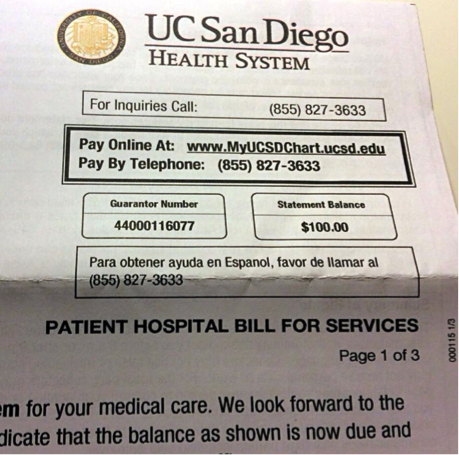
\includegraphics[width=0.5\textwidth]{Pics/insurance_receipt}
\caption{UC San Diego Health System 的醫療帳單。}
\end{figure}

上面有金額,還有一個 pay online,照著 instruction 走,就可以繳費了。

\item[Step 3.] 看完急診後,學校會是情況而定你是否需要再繼續追蹤,如果要的話,他會給你一張 referral 單子,照著這張,然後電話預約想去的醫院和時段,一樣是收 \$20 的掛號費\footnote{如果需要請假證明,可以請醫師開 work/school absence certificate,是免費的。}。
\end{enumerate}

\item dental insurance(company:Delta Dental)

%\begin{center}
%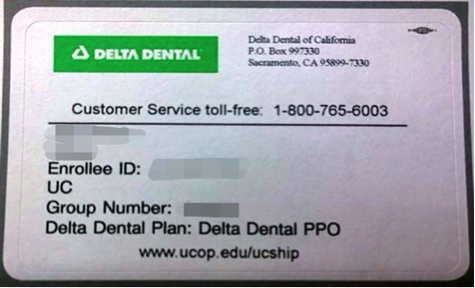
\includegraphics[width=0.5\textwidth]{Pics/dental_insurance_card}
%\end{center}

\begin{itemize}
\item 自付額(掛號費):\$25。
\item 一些免費的項目(也不需要掛號費的):oral examinations, routine cleanings, x-rays, fluoride treatment, space maintainers, specialist consultations.
\item 如果有遇到嚴重點的狀況(像填牙,蛀牙,牙齦治療,拔智齒),擁有醫療保險,你需要付的是總金額的 20\%,保險公司會幫你付剩下的 80\%。
\end{itemize}

\item vision insurance (through vision service plan)

\begin{itemize}
\item 福利:一年免費驗光一次(包含眼鏡處方簽,隱形眼鏡處方簽,校外一次 \$140,滴染劑到眼睛,檢查眼睛內部。
\item 如何配眼鏡?先到 Student Health Center 安排驗光,但是因為驗光師一周只會出現二到三次,所以要提早預約(預約基本上都是要排到兩周到一個月後)然後拿著處方簽到任何一間你想要的眼鏡店配眼鏡,學校保險會幫你 cover 鏡框的費用,所以只需要負擔鏡片的費用。
\end{itemize}

\end{enumerate}

\section{玩耍}
\subsection{景點} 

\begin{enumerate}
\item Potato Chip Rock:是在 Mount Woodson Trail 旁像馬鈴薯片一樣的石頭,需要走大約一個半小時的徒步道,才可以到達山頂,Potato Chip Rock 就位在山頂。每天吸引很多人前來拍照觀看,但是想要站在上面照相的人實在非常多,光排隊照相就要一陣子,建議早點出發。從學校開車約需要 35 分鐘才能到達爬山的起點。

\item Coronado Island:Coronado Island 最最有名的就是 Hotel del Coronado,是個拍過很多電影,又充滿復古風的飯店,鄰近沙灘。另外渡船頭附近也有很多特色小店,從這邊望過去 San Diego downtown 有美麗的夜景,非常推薦。可以選擇在 San Diego 市區搭渡輪到 Coronado Island,或者是走 5 號州際公路接 75 號,再行經 Coronado Bridge 就到了。

\item Midway Museum:中途島號航空母艦是美國海軍的航空母艦,後來被民間收購之後,改裝成博物館供民眾參觀。博物館位於San Diego downtown 旁的碼頭,是航空迷必到之處,船頂有放幾架飛機讓大家拍照。它前面的雕像是根據著名的新聞圖片「勝利之吻」而建立的,這座雕像大约 8、9 公尺高,穿深色海軍服的士兵激情地擁吻女護士。來 San Diego 沒有到這雕像就不算來過唷,從學校開車大約 18 分鐘可以到達。

\item Old Town San Diego:Old Town 是 San Diego County 的歷史遺址,建築主要是以墨西哥/西班牙風格為主,這是因為加州早期有一段時間和墨西哥同為西班牙殖民地的緣故,當地不少建築根據考據修復成原先的樣貌,有些則真的是從以前保存下來的老舊建築,但其他小屋則多已經改成餐廳或販賣墨西哥風的小紀念品的商店,這裡可以找到很多骷顱外觀的飾品,為墨西哥阿茲提克藝術的常見主題。開車從學校接 5 號州際公路,在 Old Town 出口下,即可到達,也可從校內 Gilman 公車站搭乘 150 前往,此路線為 bus sticker 免費公車路線之一。


\item Seaport Village:位在航空母艦博物館旁邊,海岸旁邊的人行步道有時有街頭藝人表演樂器、演奏、唱歌和吞劍,附近也有很多小的特色小店像是賣紀念品、辣椒、襪子、帽子,或是餐廳和小攤販可以覓食,可以邊在海邊吹吹海風看看風景。

\begin{figure}
\centering
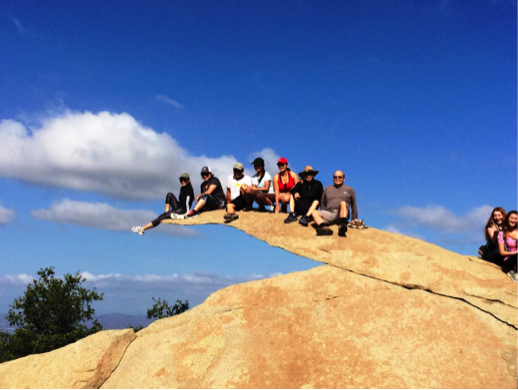
\includegraphics[width=0.45\textwidth]{Pics/potato_chip}
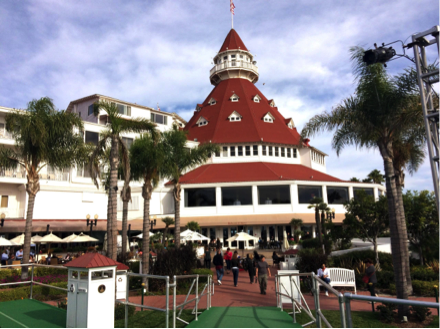
\includegraphics[width=0.45\textwidth]{Pics/coronado}\\
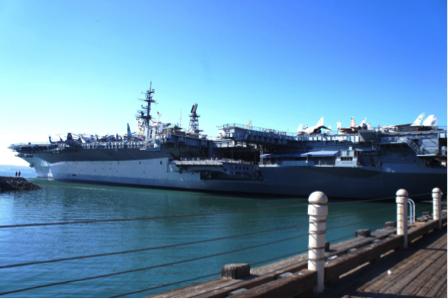
\includegraphics[width=0.625\textwidth]{Pics/midway_1}
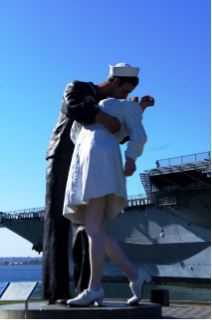
\includegraphics[width=0.275\textwidth]{Pics/midway_2}\\
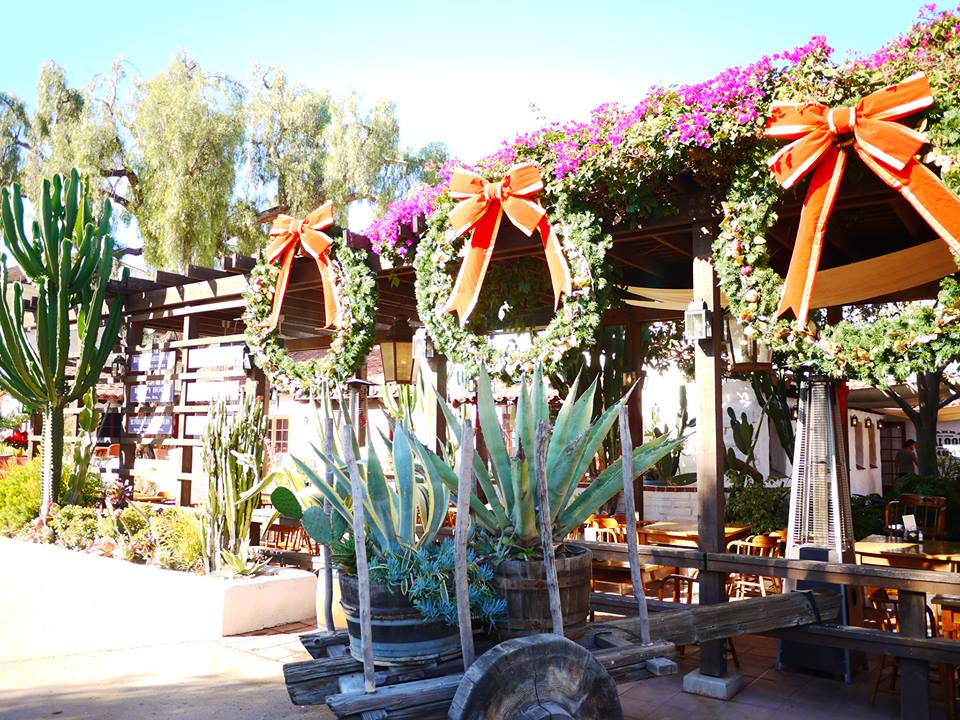
\includegraphics[width=0.42\textwidth]{Pics/oldtownsd}
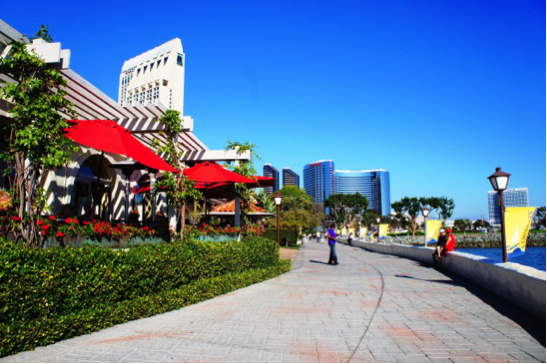
\includegraphics[width=0.48\textwidth]{Pics/seaport_village}
\caption{San Diego 著名的觀光景點(I)。(左上)Potato Chip Rock。(右上) Coronado Island 上的 Hotel del Coronado。(中左)USS Midway 中途島號航空母艦以及(中右)勝利之吻雕像。(左下)Old Town San Diego。(右下)Seaport Village。}
\end{figure}

\item San Diego Zoo:為世界知名的大型動物園,在聖地牙哥市中心的 Balboa Park 內。動物園面裡面收藏了八百餘種、超過四千隻動物。其中大熊猫,北極熊最有名,但也有像大象,老虎,河馬,無尾熊等常見的動物。 開車約 20 分鐘可以到達。

\item Safari Park:位於 San Diego Downtown 北邊,為了飼養許多野生動物所以腹地遼闊。園內飼養許多包括來自全球各地的野生瀕危動物,基本上是搭車遊覽,若想要更接近野生動物例如餵食或要去摸牠們都需要另外付費。

\item Sea World:是很有名的海洋生物主題樂園,在離學校不遠的 Mission Bay 旁。可觀賞殺人鯨,海豚,海豹等表演也可以搭乘雲霄飛車等遊樂設施。San Diego 的 Sea World 表演和設施都非常精彩,但是由於在海邊天氣較冷,較推薦夏天的時候前往。

\item Balboa Park:是 San Diego 歷史悠久的文化公園,園區裡面包含了各式各樣的博物館、植物園、花園等等,有些園區要付費才能進入有些不用,如果有要參觀博物館或是歐式花園建築,會花到一天的時間。如果只是像逛街一樣走走,二、三個小時就可以拍到美美的風景建物。從學校一路往南,大約開 20 分鐘就可以到達。

\item Julian:位於San Diego東北邊的小鎮,以盛產蘋果及蘋果製品著名,蘋果派、apple cider 都十分新鮮美味,但也價格不斐,秋天是最適合前往拜訪的季節。

\item Point Loma:SAN 機場西方往南延伸出去的小半島,上半段為軍事管制區,下半段則為 Cabrillo National Monument,入園需收費,有小巧的燈塔及回望 San Diego 市區美景,大約可以安排兩個小時在此。

\item Soledad Park:算是 La Jolla 地區的至高點之一,有個巨大的十字架地標,可以俯瞰 La Jolla shore,據說晚上是個尚可的觀星地點,但在美國無論何地晚上出門都要特別注意安全。
\end{enumerate}

\begin{figure}[H]
\centering
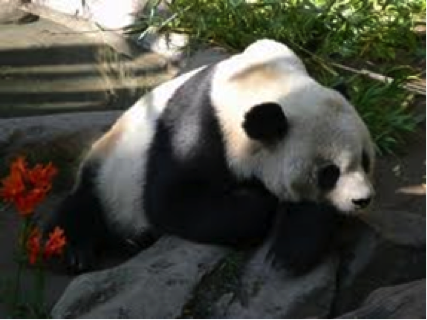
\includegraphics[width=0.45\textwidth]{Pics/san_diego_zoo}
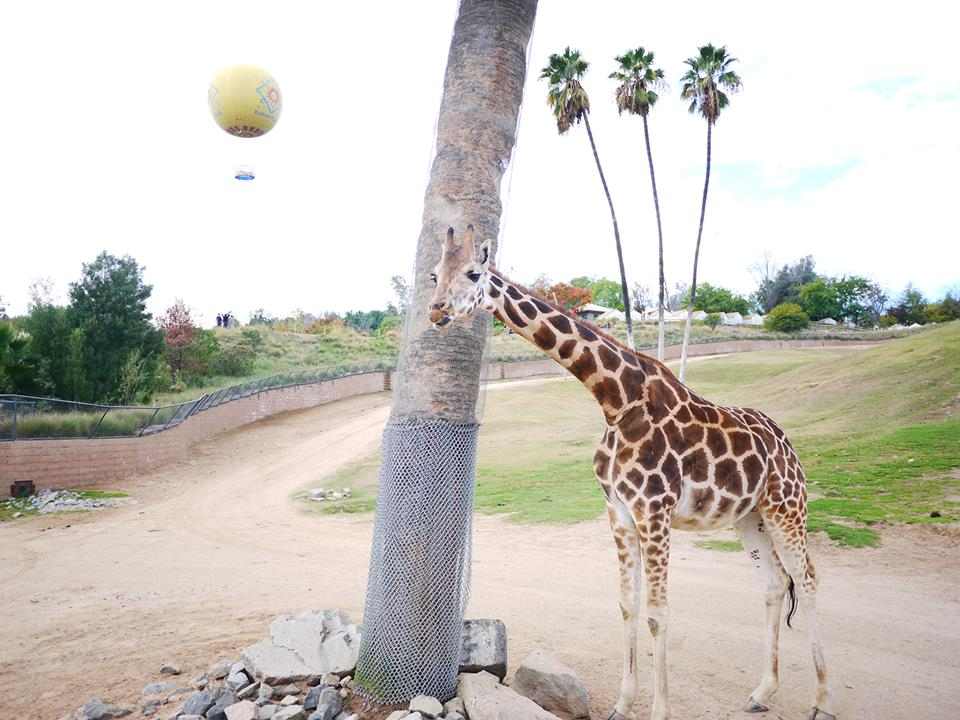
\includegraphics[width=0.45\textwidth]{Pics/sdzoo1}\\
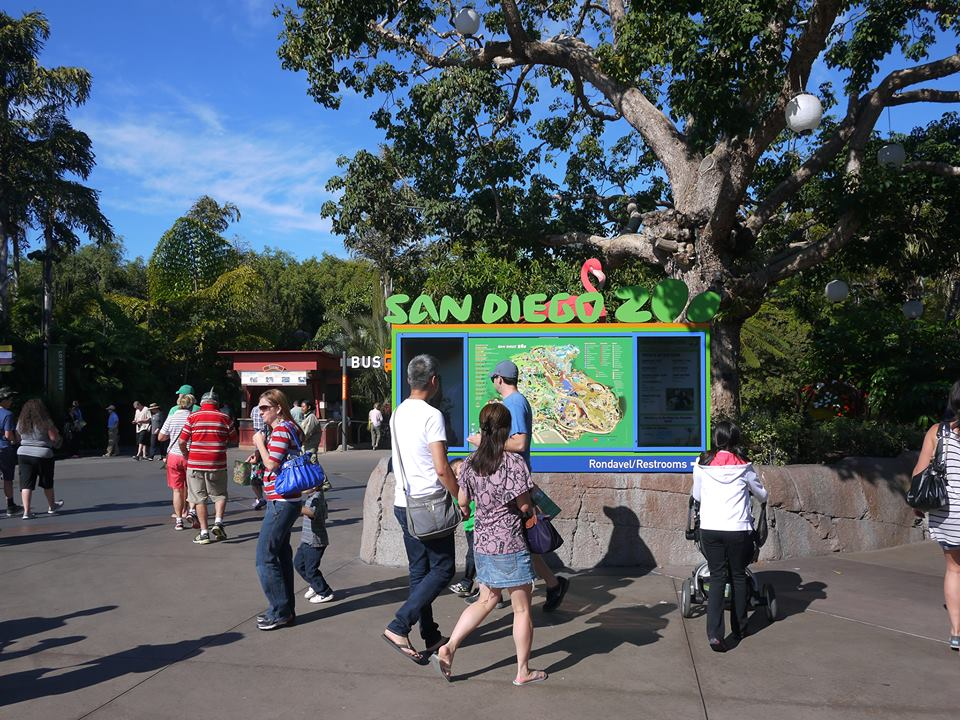
\includegraphics[width=0.395\textwidth]{Pics/sdzoo2}
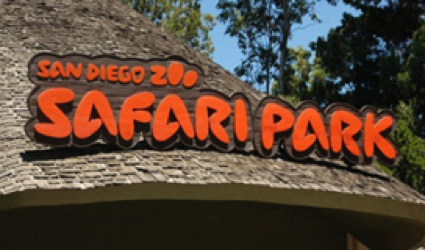
\includegraphics[width=0.505\textwidth]{Pics/safari_park}\\
\includegraphics[width=0.45\textwidth]{Pics/sea_world}
\includegraphics[width=0.45\textwidth]{Pics/balboa_park}
\caption{San Diego 著名的觀光景點(II)。(上)San Diego Zoo 的動物們以及(中左)遊玩人潮 。(中右)野生動物園 Safari Park。(左下)Sea World 精彩的殺人鯨表演。(右下)San Diego 歷史悠久的文化公園---Balboa Park 。以上部份圖片引用網路資源:\url{http://www.towngoodies.com/town:us-ca-san-diego/p/3}、\url{http://sandiegosol.com/internationalgames/san-diego-attractions/}、\url{http://www.entersandiego.com/seaworld.cfm}、\url{http://blog.visitsandiego.com/tag/balboa-park/}。}
\end{figure}

\subsection{海灘} 
\begin{enumerate}
\item La Jolla Cove:就位於學校旁的海灘,以海豹(海狗?海獅?)躺在沙灘上聞名,但是他們的叫聲和味道也是令人印象深刻。(可搭乘 30 號公車前往,為 bus sticker 免費公車路線之一。)

\item La Jolla Shore:鄰近La Jolla Cove附近的沙灘,沙灘上面會有很多人躺著曬日光浴。旁邊也有一些小店。(可搭乘 30 號公車前往,為 bus sticker 免費公車路線之一。)

\item Mission Bay:傍晚的雲彩倒映在海上很美,會呈現彩色的。旁邊的草坪可以烤肉和露營,也有很多帆船會出現,旁邊也是以沙岸為主。

\item Sunset Cliff:號稱看夕陽最美麗的景點。

\item Pacific Beach:位於 La Jolla Shore 在南端一底的沙灘,有長長的堤防,旁邊一樣有小店可以逛逛走走。 (可搭乘 30 號公車前往,為 bus sticker 免費公車路線之一。)

\item Torrey Pines:在校園的西北邊開車約莫15分鐘可到,是一長條的沿海峭壁,有不少特別的鳥類居住在此。由於海岸線平緩且風景優美,假日總是車滿為患,建議平日前來,其步道難度中等,如不願步行也可付費開車上崖壁。

\item Black's Beach:是加州知名的天體營所在地,位置就在Salk Institute西邊下峭壁的海灘,任何人都可以前往,也不會強制要加入天體活動,但記得不要對人拍照是最基本的禮貌。
\end{enumerate}

\begin{figure}[H]
\centering
\includegraphics[width=0.45\textwidth]{Pics/la_jolla_cove}
\includegraphics[width=0.45\textwidth]{Pics/la_jolla_shore}\\
\includegraphics[width=0.475\textwidth]{Pics/mission_bay}
\includegraphics[width=0.425\textwidth]{Pics/missionbay}\\
\includegraphics[width=0.395\textwidth]{Pics/sunset_cliff}
\includegraphics[width=0.505\textwidth]{Pics/pacific_beach}
\caption{UC San Diego 附近的海灘。(左上)La Jolla Cove 。(右上)La Jolla Shore。(中左、中右)Mission Bay。(左下)Sunset Cliff、(右下)Pacific Beach 。以上部份圖片引用網路資源:\url{http://yetsai.blogspot.com/2009/09/san-diego-la-jolla-cove-childrens-pool.html}、\url{http://creative--dragon.deviantart.com/art/Sunset-Cliffs-LE-6-243567878}。}
\end{figure}

\section{TGSA活動介紹}

TGSA為服務台灣學生,會在學期中提供大大小小的活動.以下是主要的幾個活動簡介:
\begin{enumerate}

\item{新生說明會:}在台灣每年都會為新生準備新生說明會,通常會在7月初舉辦,提供新生面對面問學長姐和認識新同學的機會。

\item{實習說明會:}
大約在 9 月底,TGSA 會為新生舉辦實習說明會,會請來有成功找到實習或者已經在業界的學長姊分享經驗和找實習的注意事項,幫助新生找到暑期實習。Fall quarter 的 job fair 是最大的一個,大約在開學半個月後,10 月中到底左右。

\item{雙十盃壘球:}
大約在 10 月初,南加州都會舉辦壘球聯誼賽,TGSA都會派一隊去參加,有興趣的新生也歡迎加入。

\item{小迎新:}
每年TGSA都會舉辦小迎新,歡迎新生正式加入 UCSD 的大家庭,會有新生與上一屆的學長姐參加,並希望新生跟學長姐們可以多交流互動,小迎新大概辦在 fall quarter 剛開學後。

\item{大迎新:}
大迎新大約會辦在 fall quarter 期中考前,活動會邀請居住在 San Diego 的台灣人參加,讓新生有機會跟這邊的台灣人交流。

\item{春節晚會:}
春節是一個團圓的節日,很可惜 UCSD 是三學期制,台灣在過春節時通常我們都還在上課,但不用擔心,TGSA 也有舉辦春節晚會,為在 UCSD 打拼台灣同學舉辦圍爐,現場還有抽獎活動,有興趣的同學們不要錯過了。

\item{排球團:}
TGSA 每個星期都會在學校的室內體育館練習排球,喜歡打排球的同學們千萬不要錯過了!

\item{羽球團:}
TGSA 每個星期都會在學校的室內體育館練習羽球,喜歡打羽球的同學們千萬不要錯過了!

\item{籃球團:}
TGSA 每個星期都會在學校的室內體育館練習籃球,喜歡打籃球的同學們千萬不要錯過了!

\end{enumerate}

\glsaddall


\backmatter
\newpage
\end{CJK}

\end{document}